%------------------------------------ IMPORTS ---------------------------------------%
\documentclass[a4paper,12pt]{article}

\usepackage[a4paper, top=1.5cm, bottom=1.5cm, left=2.1cm, right=2.1cm]{geometry}
\usepackage{color}
\usepackage{graphicx}
\graphicspath{{./images/}}
\usepackage{titlesec}
\usepackage{fancyhdr}
\usepackage{tikz}
\usepackage{everypage}
\usepackage{setspace}
\usepackage{lipsum}
\usetikzlibrary{positioning}
\usepackage{url}
\usepackage{float}

%------------------------------------- PREAMBLE --------------------------------------%

\pagestyle{fancy}
\fancyhf{}
\cfoot{\thepage}
\renewcommand{\headrulewidth}{0pt}
\setstretch{1.25}


\AddEverypageHook{%
  \begin{tikzpicture}[remember picture, overlay]
    \draw[line width=1pt]
      ([xshift=1.2cm,yshift=-1cm]current page.north west) rectangle
      ([xshift=-1.2cm,yshift=1cm]current page.south east);
  \end{tikzpicture}
}


%----------------------------------- TITLE PAGE ---------------------------------------%
\begin{document}
\pagenumbering{roman}
\begin{center}
\vspace*{0.5cm}

\textbf{\LARGE SAMASTHA - IELTS MOCK}

\vspace{0.7cm}

\textit{\large A project report submitted in}\\
\vspace{0.2cm}
\textit{\large Partial fulfillment for award of the degree of}

\vspace{0.8cm}

\textbf{\LARGE BACHELOR OF TECHNOLOGY}

\vspace{0.5cm}

in

\vspace{0.5cm}

\textbf{\Large Department of Computer Science and Engineering}

\vspace{1cm}

\textbf{Submitted by}

\vspace{0.5cm}

\textbf{B Mallesh (N190861)}

\vspace{1cm}

\textbf{Under the Esteemed Guidance of}

\vspace{0.5cm}

\textbf{Mr. R. Siva Narayana}\\
Assistant Professor

\vspace{2cm}


\includegraphics[width=3cm]{images/logo4.jpeg}

\vspace{1cm}

\textbf{DEPARTMENT OF COMPUTER SCIENCE ENGINEERING}\\
\vspace{0.3cm}
Rajiv Gandhi University of Knowledge Technologies – Nuzvid\\
Nuzvid, Eluru(Dist), Andhra Pradesh – 521202.

\end{center}



%-------------------------- CERTIFICATE OF COMPLETION PAGE ---------------------------%
\newpage
\begin{center}
\begin{minipage}{0.1\textwidth}

\includegraphics[width=1.8cm]{images/logo4.jpeg}
\end{minipage}
\hspace{0.5cm} % small horizontal space
\begin{minipage}{0.85\textwidth}
\centering
\textbf{DEPARTMENT OF COMPUTER SCIENCE ENGINEERING}\\
\vspace{0.2cm}
Rajiv Gandhi University of Knowledge Technologies – Nuzvid\\
Nuzvid, Eluru(Dist), Andhra Pradesh – 521202.
\end{minipage}
\end{center}

\vspace{0.5cm}
\noindent\rule{17cm}{0.4pt}

\vspace{0.5cm}
\begin{center}
\underline{\textbf{\Large CERTIFICATE OF COMPLETION}}
\end{center}

\vspace{1cm}

\noindent
This is to certify that the work entitled, \textbf{“SAMASTHA - IELTS MOCK”} is the bonafide work of \textbf{B Mallesh (N190861)}, carried out under my guidance and supervision for 4\textsuperscript{th} year major project of \textbf{Bachelor of Technology} in the Department of Computer Science and Engineering under RGUKT IIIT Nuzvid. This work is done during the academic session July 2024 - April 2025, under our guidance.

\vspace{9cm}

\begin{minipage}{0.45\textwidth}
\raggedright
\vspace{0.5cm}
\begin{tikzpicture}
\draw[dotted, thick] (0,0) -- (6,0);
\end{tikzpicture}\\
\textbf{Mr. Racharla Siva Narayana}\\
Assistant Professor,\\
Department of CSE,\\
RGUKT-Nuzvid.
\end{minipage}
\hfill
\begin{minipage}{0.45\textwidth}
\raggedleft
\vspace{0.8cm}
\begin{tikzpicture}
\draw[dotted, thick] (0,0) -- (6,0);
\end{tikzpicture}\\
\textbf{ Mrs. Samineni Bhavani}\\
Assistant Professor,\\
Head of the Department,\\
Department of CSE,\\
RGUKT-Nuzvid.
\end{minipage}



%------------------------- CERTIFICATE OF EXAMINATION PAGE ---------------------------%
\newpage
\begin{center}
\begin{minipage}{0.1\textwidth}

\includegraphics[width=1.8cm]{images/logo4.jpeg}
\end{minipage}
\hspace{0.5cm}
\begin{minipage}{0.85\textwidth}
\centering
\textbf{DEPARTMENT OF COMPUTER SCIENCE ENGINEERING}\\
\vspace{0.2cm}
Rajiv Gandhi University of Knowledge Technologies – Nuzvid\\
Nuzvid, Eluru(Dist), Andhra Pradesh – 521202.
\end{minipage}
\end{center}

\vspace{0.5cm}

\noindent
\begin{center}
\noindent\rule{17cm}{0.4pt}
\end{center}

\vspace{0.3cm}

\begin{center}
\underline{\textbf{\Large CERTIFICATE OF EXAMINATION}}
\end{center}

\vspace{1cm}

\noindent
This is to certify that the work entitled \textbf{“SAMASTHA - IELTS MOCK”} is the bonafide work of \textbf{B Mallesh (N190861)}, and hereby we accord our approval of it as a study carried out and presented in a manner required for its acceptance as Final year of \textbf{Bachelor of Technology} for which it has been submitted. This approval does not necessarily endorse or accept every statement made, opinion expressed, or conclusion drawn, as recorded in this thesis. It only signifies the acceptance of this thesis for the purpose for which it has been submitted.

\vspace{9cm}


\begin{minipage}{0.45\textwidth}
\raggedright
\vspace{0.5cm}
\begin{tikzpicture}
\draw[dotted, thick] (0,0) -- (6,0);
\end{tikzpicture}\\
\textbf{Mr. Racharla Siva Narayana}\\
Assistant Professor,\\
Department of CSE,\\
RGUKT-Nuzvid.
\end{minipage}
\hfill
\begin{minipage}{0.45\textwidth}
\raggedleft
\vspace{0.5cm}
\begin{tikzpicture}
\draw[dotted, thick] (0,0) -- (6,0);
\end{tikzpicture}\\
\textbf{Mr. Kumar Anurupam}\\
Assistant Professor,\\
Department of CSE,\\
RGUKT-Nuzvid.
\end{minipage}



%------------------------------- DECLARATION PAGE ------------------------------------%
\newpage
\begin{center}
\begin{minipage}{0.1\textwidth}

\includegraphics[width=1.8cm]{images/logo4.jpeg}
\end{minipage}
\hspace{0.5cm}
\begin{minipage}{0.85\textwidth}
\centering
\textbf{DEPARTMENT OF COMPUTER SCIENCE ENGINEERING}\\
\vspace{0.2cm}
Rajiv Gandhi University of Knowledge Technologies – Nuzvid\\
Nuzvid, Eluru(Dist), Andhra Pradesh – 521202.
\end{minipage}
\end{center}

\vspace{0.5cm}

\noindent
\begin{center}
\noindent\rule{17cm}{0.4pt}
\end{center}

\vspace{0.3cm}

\begin{center}
\underline{\textbf{\Large DECLARATION}}
\end{center}

\vspace{1cm}

\noindent
I, \textbf{B Mallesh (N190861)} hereby declare that the project report entitled \textbf{“SAMASTHA - IELTS MOCK”} done by me under the guidance of \textbf{Mr. R. Siva Narayana}, Assistant Professor, is submitted for the partial fulfillment for the award of degree of \textbf{Bachelor of Technology} in Computer Science and Engineering during the academic session July 2024 – April 2025 at RGUKT-Nuzvid.

\vspace{0.8cm}

\noindent
I also declare that this project is a result of my own effort and has not been copied or imitated from any source. Citations from any websites are mentioned in the references. The results embodied in this project report have not been submitted to any other university or institute for the award of any degree or diploma.

\vspace{6cm}


\begin{minipage}{0.45\textwidth}
\textbf{Date  :} \today\\
\textbf{Place :} Nuzvid
\end{minipage}
\hfill
\begin{minipage}{0.45\textwidth}
\raggedleft
\textbf{B Mallesh (N190861)}
\end{minipage}




%-------------------------------- ACKNOWLEDGEMENT -------------------------------------%

\newpage
\begin{center}
\vspace*{1cm}
\textbf{\LARGE ACKNOWLEDGMENT}
\end{center}

\vspace{1cm}
\noindent
I would like to express my profound gratitude and deep regards to my guide \textbf{Mr. R. Siva Narayana} for his exemplary guidance, monitoring, and constant encouragement throughout the B.Tech course. I shall always cherish the time spent with him during the course of this work due to the invaluable knowledge gained in the field of software development.

\vspace{0.5cm}
\noindent
I am extremely grateful for the confidence bestowed upon me and for entrusting me with my project entitled \textbf{“SAMASTHA - IELTS MOCK”}.

\vspace{0.5cm}
\noindent
I express my gratitude to \textbf{Mrs. Samineni Bhavani} (Head of the Department, CSE) and other faculty members for being a source of inspiration and constant encouragement, which helped me in completing the project successfully.

\vspace{0.5cm}
\noindent
Finally, yet importantly, I would like to express my heartfelt thanks to my beloved God and parents for their blessings, and my friends for their help and wishes for the successful completion of this project.

% \vspace{1.5cm}
% \noindent
% \textbf{B Mallesh (N190861)}



%------------------------------ TABLE OF CONTENTS ------------------------------------%
\newpage
\tableofcontents
% \thispagestyle{empty}
\addtocontents{toc}{\protect\thispagestyle{empty}}

%------------------------------ LIST OF FIGURES --------------------------------------%
\newpage
\listoffigures
% \thispagestyle{empty}
\addcontentsline{toc}{section}{List of Figures}


%-------------------------------- ABSTRACT PAGE --------------------------------------%
\newpage
\pagenumbering{arabic}
\phantomsection
\addcontentsline{toc}{section}{ABSTRACT}
\begin{center}
\textbf{\LARGE ABSTRACT}
\end{center}

\vspace{1cm}

\noindent
\textbf{SAMASTHA - IELTS Mock} is an AI-powered IELTS preparation platform designed to replicate the official IELTS exam experience through an adaptive, interactive, and feedback-driven approach. This system encompasses all four key IELTS modules — Listening, Reading, Writing, and Speaking — offering timed practice sessions and dynamic feedback mechanisms.

\vspace{0.5cm}

The platform integrates intelligent features such as AI voice synthesis, automatic speech recognition, dynamic feedback analysis, grammar and spelling validations, and performance-based dashboards. Each module includes section-wise instructions, practice environments, and simulated test conditions to ensure thorough preparation.

\vspace{0.5cm}

Listening modules are segmented into 4 parts, including conversations and monologues, with AI-audio-based responses and synchronized text display. Speaking tasks involve AI-conducted interviews, timed recordings, and intelligent assessments across fluency, coherence, pronunciation, and vocabulary.

\vspace{0.5cm}

The Reading and Writing modules provide comprehension-based assessments and structured tasks with real-time word counters and grammar validation. At the end of each test, users receive personalized feedback, band scores, and visual reports highlighting strengths and improvement areas.

\vspace{0.5cm}

This project aims to provide an enhanced learning experience for IELTS aspirants by merging modern technology with academic assessment strategies — thus empowering users to evaluate and elevate their English proficiency before appearing for official IELTS exams.

\vspace{1.5cm}


%--------------------------------- INTRODUCTION --------------------------------------%
\newpage
\section{Introduction}

\vspace{0.5cm}

The International English Language Testing System (IELTS) stands as one of the most widely recognized and accepted assessments of English language proficiency across the globe. It is a standardized test that plays a crucial role in shaping the academic, immigration, and professional pathways of millions of candidates. As the demand for overseas education and international opportunities continues to rise, the importance of well-structured IELTS preparation tools has become paramount. In response to this evolving need, \textbf{SAMASTHA - IELTS MOCK} has been conceptualized and developed as a modern digital platform. Leveraging the power of artificial intelligence and intelligent automation, the platform emulates the real-world IELTS test environment and offers aspirants a highly immersive, accessible, and self-adaptive testing experience. The project is aimed at delivering end-to-end support for all four key components of the IELTS exam — Listening, Reading, Writing, and Speaking — while addressing common barriers such as affordability, personalization, and real-time performance insights.

\vspace{0.5cm}

\subsection{Motivation}

The inception of this project was primarily driven by the challenges encountered by a vast number of IELTS aspirants. Traditional methods of test preparation often involve attending offline coaching centers, purchasing costly material, or relying on static mock tests that fail to adapt to individual learning needs. Moreover, many learners lack access to on-demand practice tools that provide detailed analysis or actionable feedback, particularly in writing and speaking — the most subjective components of the exam. This gap in available resources highlighted the need for a more responsive and intelligent system. \textbf{SAMASTHA - IELTS MOCK} was thus envisioned as an AI-powered solution that democratizes test preparation by offering an affordable, efficient, and exam-oriented platform. It caters to individual learners' needs and allows them to gain familiarity with test patterns while continuously improving their skills based on targeted feedback.

\vspace{0.5cm}

\subsection{Objectives}

The core objective of this project is to design and implement a digital platform that closely replicates the official IELTS examination process through smart automation. The platform seeks to enable learners to take mock tests that are not only structured in accordance with IELTS standards but also dynamically responsive to user inputs. It is built to provide a highly realistic test experience that simulates conditions such as time constraints, audio prompts, and written instructions. In addition to offering module-wise and full-length tests, the system integrates AI services to evaluate user inputs, especially for writing and speaking sections, and generates personalized feedback and band score estimations. Furthermore, the project aims to create a performance tracking system that helps users visualize their learning progress, pinpoint recurring mistakes, and measure their readiness over time.

\vspace{0.5cm}

\subsection{Scope of the Project}

The platform is designed to support a wide range of test scenarios that reflect the different modules of the IELTS examination. For the Listening module, the system utilizes AI-generated audio, where questions are synchronized with transcript display and responses are recorded in real time. In the Reading module, users are presented with diverse comprehension tasks such as multiple-choice, sentence matching, and paragraph identification, all under strict timer control. The Writing module provides two structured tasks — task 1 for report writing based on visual data, and task 2 for essay writing — both of which are evaluated using NLP-powered grammar checks and coherence analysis. The Speaking module simulates an AI-conducted oral interview, where the user responds to timed prompts and receives fluency and pronunciation feedback. All modules are integrated with review mechanisms, progress dashboards, and history logs that allow users to track their journey from beginner to band-ready levels.

\vspace{0.5cm}

\subsection{Technology Stack}

The technology stack for \textbf{SAMASTHA - IELTS MOCK} combines modern web frameworks, cloud services, and AI integrations to ensure seamless operation and intelligent automation. The major components are outlined below:

\begin{itemize}
    \item \textbf{Frontend:} Built using \textbf{React.js}, enabling a component-based, interactive user interface.
    \item \textbf{Styling:} Implemented with \textbf{Tailwind CSS}, offering a utility-first responsive design system.
    \item \textbf{Backend:} Developed using \textbf{Python} with \textbf{FastAPI} and \textbf{Flask} for secure, scalable REST API services.
    \item \textbf{Database:} \textbf{MySQL} is used to manage user data, test results, answer history, and analytics.
    \item \textbf{Authentication:} \textbf{JWT (JSON Web Tokens)} ensures secure session management and access control.
    \item \textbf{AI and NLP Services:}
    \begin{itemize}
        \item \textbf{Google Cloud Speech-to-Text} for converting speaking responses into text.
        \item \textbf{OpenAI API} for writing evaluation, grammar checking, feedback generation, and band score prediction.
    \end{itemize}
    \item \textbf{Deployment:} 
    \begin{itemize}
        \item Frontend hosted on \textbf{Vercel}.
        \item Backend services deployed using \textbf{Render} or \textbf{Heroku}.
    \end{itemize}
\end{itemize}


\vspace{0.5cm}

\subsection{Significance of the Project}

The significance of this project lies in its potential to reshape the way students prepare for high-stakes language proficiency exams. \textbf{SAMASTHA - IELTS MOCK} offers a unique blend of accessibility, automation, and adaptability, making it a practical tool for self-learners, educational consultants, and training institutions. Unlike traditional mock exams or test books, this platform evolves with user interaction, constantly fine-tuning its recommendations and analysis based on user performance. Its ability to provide detailed analytics, instant AI-driven feedback, and visual progress charts gives users a sense of control over their preparation journey. Moreover, by replicating actual IELTS exam patterns and test timing, the platform helps reduce test-day anxiety and boosts overall confidence. It is not just a practice tool, but a personalized mentor designed to bring out the best in every aspirant.

\vspace{0.5cm}

\subsection{Conclusion}

In conclusion, the development of \textbf{SAMASTHA - IELTS MOCK} serves as a proactive response to the evolving demands of modern learners preparing for international English language examinations. By combining technology with pedagogy, the platform provides a comprehensive, user-friendly, and feedback-driven environment that encourages regular practice, measurable improvement, and long-term language mastery. The project embodies the future of language testing — smart, scalable, and centered around the learner.




\newpage
\section{Real World Applications}

\vspace{0.5cm}

The \textbf{SAMASTHA - IELTS MOCK} platform offers diverse practical applications, benefiting a wide spectrum of learners, educators, and institutions in the English language training ecosystem. By leveraging AI and automation, it bridges the gap between traditional learning tools and modern digital expectations. Below are the key real-world applications:

\vspace{0.3cm}

\begin{itemize}
    \item \textbf{IELTS Aspirants:} This platform allows test takers to simulate real exam environments with authentic timing, question patterns, and adaptive feedback. Regular usage not only builds familiarity with the exam structure but also improves time management and performance consistency — two crucial aspects of succeeding in the IELTS examination.

    \item \textbf{Educational Institutions:} Schools, colleges, and universities can embed the platform into their curriculum as part of English language proficiency programs. It can be used to assign structured practice tasks, assess student readiness, and generate analytical reports that guide targeted improvement.

    \item \textbf{Language Coaching Centers:} Coaching institutes can use the platform as a digital extension of their classroom training. With features like automated evaluation, real-time dashboards, and history tracking, instructors can efficiently monitor each student’s progress and provide tailored interventions.

    \item \textbf{Remote Learning Environments:} In geographically underserved or rural areas, students often lack access to certified IELTS trainers. This platform provides them with a self-contained, interactive, and expert-driven testing system — all from the comfort of their homes, with minimal infrastructure requirements.

    \item \textbf{Self-paced Learning:} Individual learners who prefer autonomous study can benefit from flexible access, modular testing options, and performance tracking. It enables continuous, self-regulated learning where users can revisit weak modules, retake tests, and view growth trends over time.

    \item \textbf{Skill Assessment Portals:} Beyond IELTS, the modular test engine and evaluation architecture can be adapted to other standardized English tests such as TOEFL, PTE, or even corporate-level communication assessments. This makes it a reusable framework for various language assessment scenarios.

    \item \textbf{Corporate Training Programs:} Companies recruiting or training non-native employees can utilize the platform to assess English proficiency levels relevant to job roles. Customized test templates can be created to match industry-specific communication expectations.

    \item \textbf{EdTech Integrations:} The system’s API-ready backend allows it to integrate seamlessly into Learning Management Systems (LMS) like Moodle, Google Classroom, or proprietary EdTech platforms — offering IELTS mock testing as a built-in academic service.

    \item \textbf{Government Skill Development Programs:} National or regional language improvement initiatives can adopt the platform as a tool for large-scale English training. Its analytics and reporting features help measure collective progress and identify training gaps among batches of candidates.

    \item \textbf{Academic Research and Evaluation:} Educational researchers and policy makers can use the platform's structured data and user insights to study learning behavior, test performance trends, and AI-based evaluation efficacy in language learning contexts.
\end{itemize}

\vspace{0.3cm}

By simulating the IELTS exam through AI-driven modules, timed practice, and real-time feedback, \textbf{SAMASTHA - IELTS MOCK} emerges as more than just a student project. It positions itself as a scalable, practical, and impactful solution to drive English language proficiency across diverse educational and professional domains.


\newpage
\section{Related Works / Existing Works}

\vspace{0.5cm}

Over the past decade, several online platforms and mobile applications have emerged to assist learners in preparing for the IELTS exam. These platforms offer a variety of resources such as sample questions, instructional videos, vocabulary builders, and full-length mock tests. However, despite their popularity and utility, most of these tools operate in a static and non-adaptive manner, lacking real-time feedback, AI integration, or intelligent analytics that cater to personalized learning needs. The following subsections provide a critical overview of some of the prominent platforms in the space and how \textbf{SAMASTHA - IELTS MOCK} distinguishes itself through innovation and learner-centric features.

\vspace{0.5cm}

\subsection*{1. IELTS Liz}
IELTS Liz is a well-known educational blog created by an experienced IELTS instructor. It provides free access to a wide range of study materials, tips, and sample questions primarily in written and video formats. The platform is highly regarded for its clarity in explaining grammar rules, answering techniques, and common mistakes. However, it functions more as a reference or content repository rather than a dynamic practice environment. It does not support user interaction, automated evaluation, or data-driven feedback, which are crucial for iterative learning and test readiness.

\vspace{0.3cm}

\subsection*{2. Magoosh IELTS}
Magoosh is a comprehensive test prep platform offering structured lessons, mobile apps, and practice sets for several competitive exams, including IELTS. It emphasizes learning through video tutorials and question banks, and includes features such as flashcards and vocabulary lists. While Magoosh provides a polished learning interface and quality content, it still lacks AI-powered feedback systems, particularly in evaluating speaking and writing responses. Additionally, its performance analysis tools are limited in scope, making it less effective for students seeking in-depth, skill-wise improvement metrics.

\vspace{0.3cm}

\subsection*{3. IELTS Prep App (British Council)}
This official mobile application from the British Council provides reliable test samples, tips, and module-wise practice for IELTS aspirants. It ensures content authenticity and includes timer-based quizzes that simulate test conditions. However, it offers a generic experience with limited adaptability to individual learners. Features such as automated scoring, personalized improvement plans, or in-depth performance dashboards are absent, thus restricting its usefulness as a continuous self-evaluation tool.

\vspace{0.3cm}

\subsection*{4. E2Language}
E2Language offers instructor-led IELTS training through recorded classes, live webinars, and guided practice modules. It is among the few platforms that provide a holistic IELTS course structure with expert insights. However, a significant limitation of E2Language lies in its cost barrier — much of its content is locked behind subscription tiers, making it inaccessible to economically constrained learners, especially those in rural or underprivileged regions. Furthermore, it still requires manual grading for writing and speaking assessments, thereby slowing the feedback loop.

\vspace{0.3cm}

\subsection*{5. Duolingo English Test}
Although not an IELTS-focused platform, Duolingo’s English test has gained recognition as a modern, compact alternative for English proficiency assessment. It utilizes adaptive testing mechanisms and AI-powered scoring. However, it differs substantially in format, difficulty, and objectives when compared to IELTS. It is primarily aimed at institutions accepting alternative English tests and does not align with the IELTS preparation framework. Moreover, its speaking and writing modules are minimal and do not offer the kind of detailed evaluation that IELTS aspirants typically need.

\vspace{0.5cm}

\noindent
In contrast to the platforms discussed above, \textbf{SAMASTHA - IELTS MOCK} sets itself apart through a comprehensive suite of features that embrace both modern AI technologies and the authentic structure of the IELTS exam. The key differentiators include:

\vspace{0.3cm}
\begin{itemize}
    \item \textbf{Complete Module Simulation:} It simulates the entire IELTS testing experience, covering Listening, Reading, Writing, and Speaking in their original formats with section-wise constraints, interactive interfaces, and AI-controlled behavior such as single-play audio or timer-based navigation.
    
    \item \textbf{Real-Time AI Feedback:} Unlike platforms that rely on static question banks, this system provides dynamic feedback — using Google Cloud’s Speech-to-Text and OpenAI’s NLP models — to evaluate spoken and written answers for fluency, grammar, coherence, and vocabulary usage.
    
    \item \textbf{Automated Band Estimation:} The platform calculates indicative band scores based on AI evaluations, offering learners a near-accurate sense of where they stand in terms of IELTS readiness, which most existing tools do not provide.
    
    \item \textbf{Performance Analytics Dashboard:} A dedicated dashboard tracks user attempts, module-wise history, scores, and trend graphs, empowering learners to monitor their growth over time and focus on weaker areas.
    
    \item \textbf{Accessibility and Affordability:} The system is designed with scalability and equity in mind, ensuring that learners from diverse backgrounds can access high-quality training without dependency on paid instructors or premium services.
    
    \item \textbf{Mobile and LMS Compatibility:} Its frontend and backend design allow for easy expansion into mobile apps or integration into institutional LMS platforms, making it suitable for both individual and institutional adoption.
\end{itemize}

\vspace{0.3cm}

In conclusion, while many existing IELTS prep platforms offer useful resources, they often fall short in providing a full-fledged, intelligent, and adaptive learning ecosystem. \textbf{SAMASTHA - IELTS MOCK} addresses these limitations by combining automation, personalization, and exam accuracy in a unified system. This makes it not only a viable alternative but also a forward-thinking solution in the evolving landscape of English proficiency training.


%---------------------------------- PROPOSED METHOD ----------------------------------%
\newpage
\section{Proposed Method}

\vspace{0.5cm}

\textbf{SAMASTHA - IELTS MOCK} has been conceptualized as an AI-powered web-based system that aims to simulate the complete IELTS examination experience. The proposed methodology integrates intelligent test workflows, dynamic interfaces, and real-time analytics, offering users a seamless and adaptive platform for English language proficiency enhancement. The primary objective of the proposed method is to emulate every stage of the IELTS exam — from onboarding and test navigation to personalized scoring and performance visualization — while introducing digital intelligence at every phase of user interaction. This section outlines in detail how each part of the system operates and how users engage with the platform.

\vspace{0.5cm}

\subsection{User Onboarding and Dashboard Access}

The user journey begins at the entry point of the application, where new candidates can register or existing users can log in to access the platform. The onboarding process is tightly integrated with the Samastha authentication layer, ensuring that only verified and authorized users can access the IELTS testing environment.

Upon successful login, the user is redirected to a personalized dashboard, which acts as the central control panel for all further actions. This dashboard is intelligently designed to display:
\begin{itemize}
    \item Real-time performance insights and weekly progress indicators visualized through line charts and radial graphs.
    \item Options to initiate a full-length mock test, module-specific tests, or targeted individual exercises.
    \item Interactive module cards (Listening, Reading, Writing, Speaking) which dynamically update based on usage frequency and past performance.
    \item Access to historical results, test attempt summaries, AI-generated feedback, and performance breakdowns.
\end{itemize}

The dashboard interface is responsive and intuitive, guiding users through available resources, highlighting incomplete tests, and recommending practice paths based on previous results.

\vspace{0.5cm}

\subsection{Listening Module Workflow}

The Listening module is structured to closely resemble the official IELTS audio-based evaluation format. It comprises four sequential parts, each simulating different real-life conversation contexts such as dialogues, monologues, or academic discussions.

The workflow begins with an \textbf{Audio Check and Consent} step, where the user must verify that their system audio is functioning correctly and explicitly agree to proceed with a test that permits only one-time audio playback — a critical realism feature. Following this, the user is presented with \textbf{Timed Instruction Screens} which outline the test rules and provide navigation guidance. These screens automatically progress after a countdown to ensure a timed environment.

The core of the module revolves around a \textbf{One-Time Audio Playback System}, where users listen to pre-recorded audio clips that align with accompanying questions. A unique feature here is the synchronized text highlighting that visually assists learners in following the content without disrupting the flow of concentration. As the audio plays, users must answer in real-time. Once audio ends, the system provides a limited \textbf{Review Window} (typically 1 minute), allowing final checks and edits before automatic submission.

All responses are captured and stored, with timing and accuracy data passed to the backend for later evaluation and feedback generation.

\vspace{0.5cm}

\subsection{Reading Module Workflow}

The Reading section consists of three major parts, each simulating academic and general reading tasks of increasing difficulty. Every part includes 5–8 structured paragraphs drawn from sample IELTS datasets.

Each part begins with a \textbf{Time-Bound Environment}, where the system enforces a strict 20-minute countdown that includes both reading time and response entry. During this period, users are presented with lengthy passages followed by question blocks comprising multiple-choice, sentence completion, matching headings, or True/False/Not Given questions.

One of the intelligent elements in this module is the \textbf{Dynamic Question Block Navigation}. Based on the type of questions, the system auto-groups related queries and enables users to focus on each section sequentially. This not only prevents confusion but also improves test pacing and mental clarity.

Upon completing a part, the platform initiates an animated \textbf{Loading Transition Screen}, reinforcing the structure and seriousness of the test before moving to the next part. All responses are timestamped and evaluated post-submission to ensure validity and integrity.

\vspace{0.5cm}

\subsection{Writing Module Workflow}

The Writing module is designed with two tasks that mimic the structure of the IELTS Academic and General formats:

\textbf{Task 1} presents a graphical image, chart, or map and asks the user to write a report (minimum 150 words) summarizing key trends and observations. This task must be completed within 20 minutes. \textbf{Task 2} consists of a prompt-based opinion essay, which requires the user to write at least 250 words in 40 minutes.

Key features of this module include:
\begin{itemize}
    \item A live \textbf{Real-Time Word Counter} that dynamically updates as the user types, ensuring the minimum word count requirement is met.
    \item \textbf{Copy-Paste Restrictions} to prevent external content injection and ensure genuine writing.
    \item \textbf{Auto-Save and Submission Locking}, where test data is securely stored in intervals to prevent data loss.
    \item \textbf{Post-Test Transition Screens} that prepare users for feedback or next-module redirection.
\end{itemize}

After the test, the written content is processed through NLP engines such as OpenAI’s GPT, which evaluate it for grammar, coherence, lexical resource, and task completion — returning a band score and detailed feedback report.

\vspace{0.5cm}

\subsection{Speaking Module Workflow}

The Speaking module is one of the most crucial and subjective components of the IELTS examination, designed to assess a candidate’s ability to communicate verbally in English across a range of topics and settings. In the \textbf{SAMASTHA - IELTS MOCK} platform, this module has been meticulously designed to replicate the face-to-face interview format found in actual IELTS tests. It is powered by an AI-interactive interface that mimics human examiner behavior, ensuring that candidates experience a natural and uninterrupted flow of questions.

The Speaking module is divided into three parts:

\textbf{Part 1 – Introduction and Interview:} This section comprises general introductory questions related to familiar topics such as hobbies, work, studies, family, or daily routine. These questions are delivered using AI-generated voice, creating an immersive auditory experience. Users are expected to respond fluently within a set time limit, and a countdown timer helps simulate a real-time interview setting.

\textbf{Part 2 – Long Turn (Task Card):} In this segment, the system displays a prompt or cue card containing a topic and guiding points. The candidate is given exactly one minute to prepare, during which the question remains visible but the microphone remains inactive. After the preparation time, a two-minute timer is initiated, and the system activates the microphone to record a continuous speech response. This task evaluates a user’s ability to structure thoughts, extend ideas, and speak coherently on a single topic without interruption.

\textbf{Part 3 – Discussion and Follow-up:} Building on the topic introduced in Part 2, this section includes more analytical or opinion-based questions that challenge the user’s critical thinking and language flexibility. These follow-up questions are again delivered via AI voice and require concise but well-reasoned responses, often demanding higher-level vocabulary and grammatical accuracy.

Throughout the module, user responses are recorded in real-time. The recordings are transcribed using \textbf{Google Cloud Speech-to-Text API}, ensuring accurate speech recognition. These transcriptions are then evaluated using NLP models to generate approximate IELTS band scores based on standardized rubrics. The evaluation process considers four key parameters: \textit{fluency and coherence}, \textit{lexical resource}, \textit{grammatical range and accuracy}, and \textit{pronunciation}. After processing, the platform generates detailed feedback with transcript replay, helping users review their own speech and understand the scoring rationale.

\vspace{0.5cm}

\subsection{Feedback and Result Generation}

One of the most valuable features of \textbf{SAMASTHA - IELTS MOCK} is its robust result generation and feedback delivery system, which aims to bridge the gap between mere test-taking and actionable learning. Once the user completes either a full-length mock test or a module-wise test, the platform initiates an intelligent post-processing workflow to analyze responses and generate insights.

\vspace{0.4cm}
\subsubsection{Overall Band Score}

The first output the user sees is the aggregate IELTS band score, calculated based on their performance across the four modules. This score is displayed using clean circular progress indicators alongside numerical representations, mimicking official IELTS reporting. It provides a quick yet comprehensive glance at the candidate’s readiness level.

\vspace{0.4cm}
\subsubsection{Module-wise Analysis}

For each test section — Listening, Reading, Writing, and Speaking — the system generates individual band scores, color-coded for easy interpretation. Accompanying these scores are concise diagnostic summaries explaining what went well, what was lacking, and how performance compares to previous attempts. This comparative insight is useful in tracking progress over time.

\vspace{0.4cm}
\subsubsection{Answer Breakdown and Comparisons}

In the objective modules (Listening and Reading), the user receives a full breakdown of their responses. Correct answers are highlighted, incorrect ones are annotated with explanations, and corresponding question texts are linked for clarity. This side-by-side answer comparison helps learners identify specific misunderstandings or careless mistakes and refine their strategies for future tests.

\vspace{0.4cm}
\subsubsection{Subjective Module Proficiency Metrics}

For the Writing and Speaking sections, the system goes beyond simple scoring. Using AI-generated feedback bubbles, it presents evaluations across sub-skills such as grammar, vocabulary, sentence structure, coherence, fluency, and pronunciation. Each bubble is rated visually and numerically, offering an intuitive understanding of strengths and weaknesses across multiple dimensions.

\vspace{0.4cm}
\subsubsection{Actionable Tips and Recommendations}

Based on detected patterns or repeated errors, the platform offers personalized improvement tips. These may include vocabulary recommendations, grammar corrections, coherence suggestions, or timing strategies. The guidance is aligned with the IELTS band descriptors and tailored to each user's recent performance, enabling effective self-directed improvement.

\vspace{0.4cm}

In summary, the feedback and results module transforms each mock test attempt into a meaningful learning event. It not only evaluates but educates, guiding learners toward real, measurable progress.

\vspace{0.5cm}


\subsection{Retake and History Tracking}

Users can revisit their dashboard at any point and access their test history. The system supports:
\begin{itemize}
    \item \textbf{Retake Options} which allow users to attempt full or module-wise tests again with or without feedback.
    \item \textbf{Filter Tools} to view past tests by date, module, or score range.
    \item \textbf{Result Review Mode}, where users can reanalyze their past responses and compare their answers with sample solutions or previous attempts.
\end{itemize}

Historical data is stored securely and presented using interactive graphs and score trackers, enabling longitudinal performance analysis.

\vspace{0.5cm}

\noindent
In essence, the proposed methodology for \textbf{SAMASTHA - IELTS MOCK} creates an environment that closely mirrors official IELTS testing, enhanced with real-time intelligence and digital flexibility. The flow is not only structured and rigorous but also adaptive and learner-centric — ensuring that each user receives an experience that is personal, practical, and performance-driven.


\vspace{1cm}
\subsection{System Flow Diagram}

\begin{center}
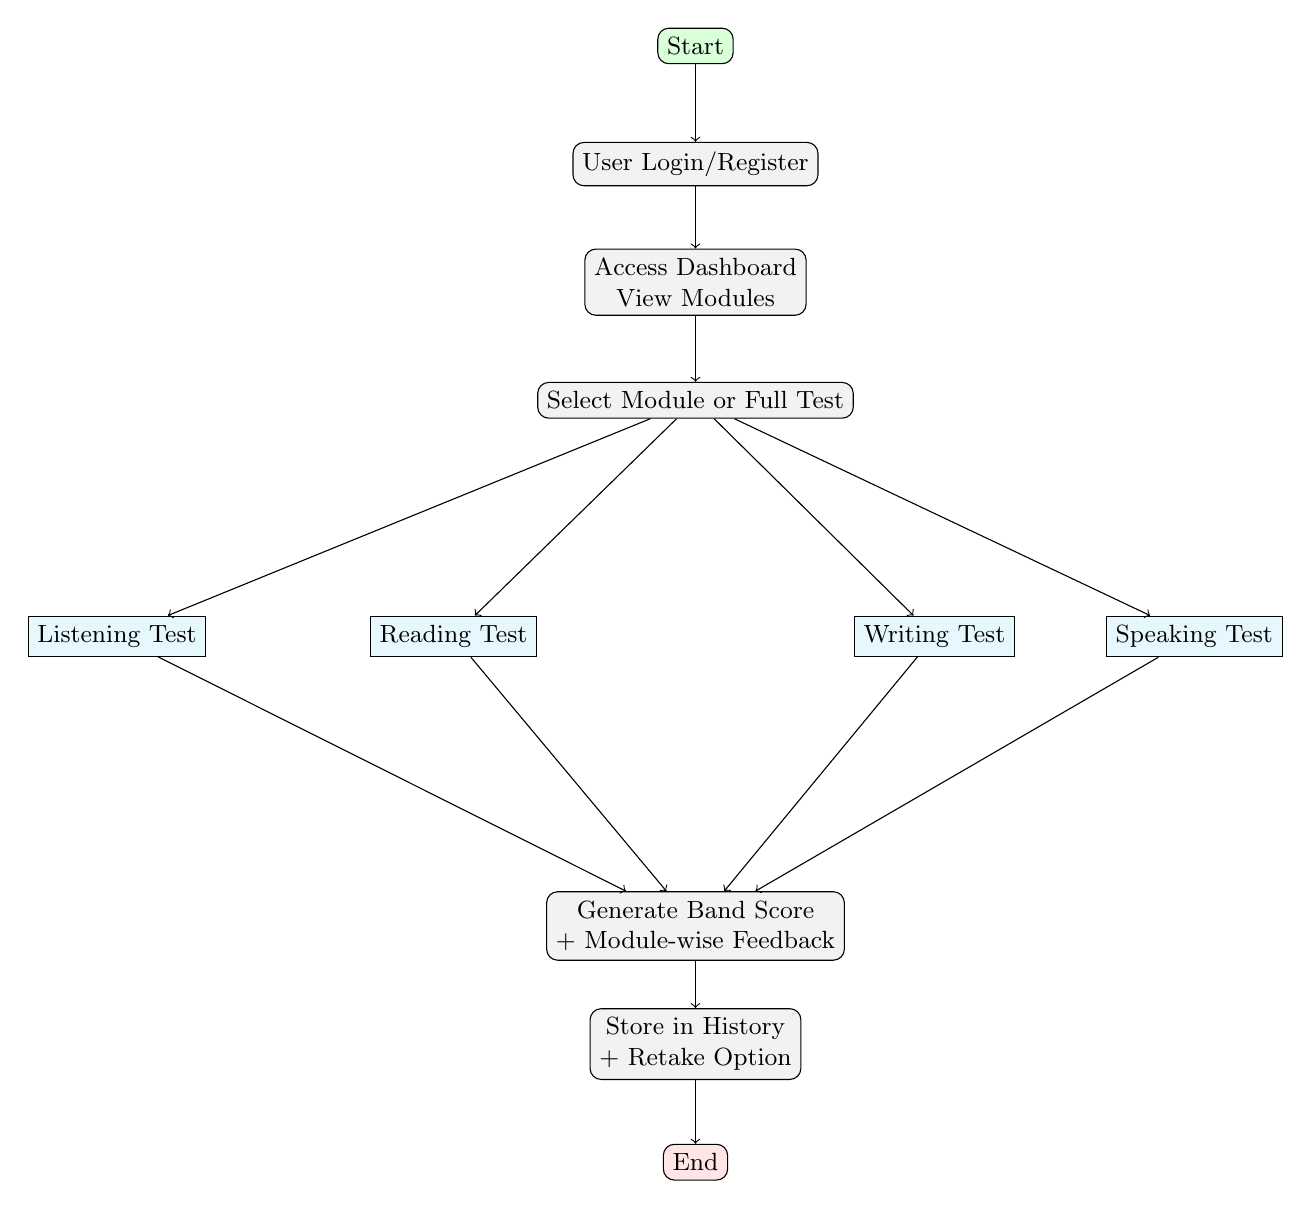
\begin{tikzpicture}[node distance=1.5cm and 1.2cm, every node/.style={align=center}, font=\small]

% Nodes
\node (start) [draw, rectangle, rounded corners, fill=green!15] {Start};
\node (login) [below of=start, draw, rectangle, rounded corners, fill=gray!10] {User Login/Register};
\node (dashboard) [below of=login, draw, rectangle, rounded corners, fill=gray!10] {Access Dashboard\\View Modules};
\node (selectTest) [below of=dashboard, draw, rectangle, rounded corners, fill=gray!10] {Select Module or Full Test};

% Horizontal Test Modules
\node (listening) [below left=2.5cm and 4.2cm of selectTest, draw, rectangle, fill=cyan!10] {Listening Test};
\node (reading) [below left=2.5cm and 0cm of selectTest, draw, rectangle, fill=cyan!10] {Reading Test};
\node (writing) [below right=2.5cm and 0cm of selectTest, draw, rectangle, fill=cyan!10] {Writing Test};
\node (speaking) [below right=2.5cm and 3.2cm of selectTest, draw, rectangle, fill=cyan!10] {Speaking Test};

\node (results) [below=6cm of selectTest, draw, rectangle, rounded corners, fill=gray!10] {Generate Band Score\\+ Module-wise Feedback};
\node (history) [below of=results, draw, rectangle, rounded corners, fill=gray!10] {Store in History\\+ Retake Option};
\node (end) [below of=history, draw, rectangle, rounded corners, fill=red!10] {End};

% Arrows
\draw[->] (start) -- (login);
\draw[->] (login) -- (dashboard);
\draw[->] (dashboard) -- (selectTest);

\draw[->] (selectTest) -- (listening);
\draw[->] (selectTest) -- (reading);
\draw[->] (selectTest) -- (writing);
\draw[->] (selectTest) -- (speaking);

\draw[->] (listening) -- (results);
\draw[->] (reading) -- (results);
\draw[->] (writing) -- (results);
\draw[->] (speaking) -- (results);

\draw[->] (results) -- (history);
\draw[->] (history) -- (end);

\end{tikzpicture}
\end{center}



%-------------------------------- SYSTEM ARCHITECTURE -------------------------------%
\newpage
\section{System Architecture}

\vspace{0.5cm}

The system architecture of \textbf{SAMASTHA - IELTS MOCK} is based on a distributed, modular, and scalable web application model. It follows a client-server architecture, enabling seamless interaction between end users and the backend services that power the platform’s intelligence. The architecture integrates modern web technologies, cloud-based NLP tools, and database systems to deliver an end-to-end IELTS simulation environment. 

This layered structure ensures that the platform is responsive, secure, extensible, and capable of handling user interactions in real time while processing large volumes of language data efficiently.

\vspace{0.5cm}
\subsection*{System Architecture Diagram}

\begin{center}
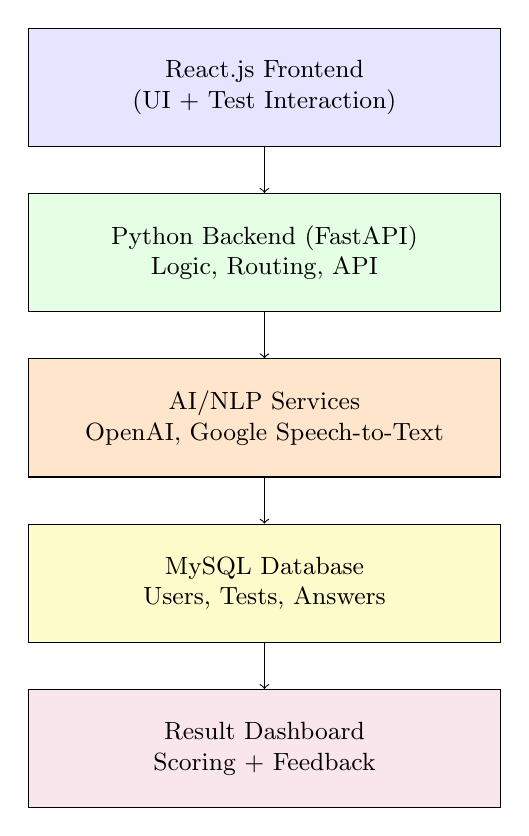
\begin{tikzpicture}[node distance=2.1cm, every node/.style={align=center, font=\small}]

% Nodes (vertical layout)
\node (frontend) [draw, rectangle, fill=blue!10, minimum width=6cm, minimum height=1.5cm] {React.js Frontend\\(UI + Test Interaction)};
\node (backend) [below of=frontend, draw, rectangle, fill=green!10, minimum width=6cm, minimum height=1.5cm] {Python Backend (FastAPI)\\Logic, Routing, API};
\node (ai) [below of=backend, draw, rectangle, fill=orange!20, minimum width=6cm, minimum height=1.5cm] {AI/NLP Services\\OpenAI, Google Speech-to-Text};
\node (database) [below of=ai, draw, rectangle, fill=yellow!20, minimum width=6cm, minimum height=1.5cm] {MySQL Database\\Users, Tests, Answers};
\node (dashboard) [below of=database, draw, rectangle, fill=purple!10, minimum width=6cm, minimum height=1.5cm] {Result Dashboard\\Scoring + Feedback};

% Arrows
\draw[->] (frontend) -- (backend);
\draw[->] (backend) -- (ai);
\draw[->] (ai) -- (database);
\draw[->] (database) -- (dashboard);

\end{tikzpicture}
\end{center}

\vspace{0.5cm}

\subsection{Frontend (Client Interface)}

The frontend serves as the user-facing interface of the system and is developed using \textbf{React.js}, a modern JavaScript library for building responsive single-page applications. \textbf{Tailwind CSS} is used to ensure design consistency and mobile responsiveness across screen sizes. The frontend handles the complete user interaction lifecycle, which includes:

\begin{itemize}
    \item Rendering timed IELTS practice interfaces across four modules: Listening, Reading, Writing, and Speaking.
    \item Managing test flows including welcome screens, instruction pages, and submission steps.
    \item Integrating voice recording features for the Speaking module using HTML5 media APIs.
    \item Dynamically displaying feedback, charts, band scores, and recommendations after test completion.
    \item Establishing secure communication with the backend through RESTful APIs, exchanging JSON data for real-time operations.
\end{itemize}

The frontend is hosted via Vercel, which supports automatic deployments, global CDN distribution, and continuous integration for rapid updates.

\vspace{0.3cm}

\subsection{Backend (Application Server)}

The backend forms the application logic layer and is developed using \textbf{FastAPI}, a high-performance Python framework that supports asynchronous request handling. FastAPI is chosen for its simplicity, built-in documentation, speed, and excellent support for modern web standards like OpenAPI and JWT authentication.

Key responsibilities of the backend include:

\begin{itemize}
    \item Managing test lifecycle routes — from start to completion — for all modules.
    \item Validating user identity and session integrity using JWT-based authentication.
    \item Routing requests to appropriate microservices or AI APIs based on test type.
    \item Processing and storing user submissions, timestamps, and partial progress.
    \item Handling feedback generation via AI model integrations and formatting results for display.
\end{itemize}

The backend is stateless, scalable, and deployed on Render or Heroku for high availability and fault tolerance. API endpoints are well-structured and versioned for future enhancements.

\vspace{0.3cm}

\subsection{Database Layer (MySQL)}

All persistent data storage is handled via a structured relational database system — \textbf{MySQL}. This layer ensures that all critical user data is securely stored and retrievable in a normalized format for analytics and user history tracking.

The database schema is designed to support the following:

\begin{itemize}
    \item Storage of user profiles, login credentials (hashed), and access roles.
    \item Detailed tracking of test attempts, start/end timestamps, and band scores per module.
    \item Storage of question pools, including correct answers, difficulty levels, and categories.
    \item Logging of AI-generated feedback, enabling retrospective analysis and comparison.
    \item Efficient retrieval for dashboard rendering and filtering based on date, module, or score.
\end{itemize}

Indexes are used for fast querying on high-read tables like test history. Additionally, foreign key constraints ensure referential integrity between user and test records.

\vspace{0.3cm}

\subsection{AI/NLP Services (External Integration)}

The intelligence layer of the system leverages third-party APIs to perform natural language processing and automated evaluation. These services are invoked from the backend, and results are fetched securely using authenticated API keys.

\begin{itemize}
    \item \textbf{Google Cloud Speech-to-Text:} This service transcribes spoken audio from the Speaking module into text with high accuracy. It supports real-time streaming, noise suppression, and language adaptation for Indian accents.
    
    \item \textbf{OpenAI API:} GPT models are used to analyze writing submissions. They evaluate grammatical accuracy, coherence, vocabulary range, and task completion. The models also generate structured feedback and suggestions to improve writing performance.
\end{itemize}

These integrations are encapsulated in the backend service layer, allowing modular interaction, API switching, and error fallback handling without exposing credentials or internal logic to the frontend.

\vspace{0.3cm}

\subsection{Feedback & Dashboard Engine}

The final layer in the architecture is responsible for rendering meaningful analytics and feedback to users after test completion. It is tightly integrated with both the database and AI evaluation pipelines.

Responsibilities include:

\begin{itemize}
    \item Aggregating raw scores into an IELTS band format using calibrated scoring metrics.
    \item Displaying results using pie charts, progress bars, and textual breakdowns.
    \item Categorizing scores into strength and weakness zones using color-coded visuals.
    \item Offering contextual feedback, sample answers, and retake pathways.
    \item Supporting user-specific data tracking to visualize growth across multiple attempts.
\end{itemize}

This component transforms raw data into actionable insights, helping users not only understand their current proficiency but also define personalized learning goals.

\vspace{0.5cm}

\noindent
In summary, the architecture of \textbf{SAMASTHA - IELTS MOCK} showcases the integration of modern web frameworks, cloud-based AI services, and real-time feedback mechanisms. The system is designed for reliability, flexibility, and educational effectiveness — ensuring that learners across the globe can access, attempt, and improve their English language skills through a self-paced, intelligent, and scalable digital platform.


%---------------------- MODULE-WISE FUNCTIONAL DESCRIPTION ---------------------------%
\newpage
\section{Module-Wise Functional Description}

\vspace{0.5cm}

This section provides a detailed breakdown of the functional flow, user interaction, and intelligent automation integrated within each IELTS module on the \textbf{SAMASTHA - IELTS MOCK} platform. These modules closely align with the structure outlined in the Functional Requirements Document (FRD) and follow the official IELTS pattern. Each module has been engineered to simulate the actual testing conditions while leveraging artificial intelligence to offer feedback and performance analytics.

\vspace{0.4cm}
\subsection{Listening Module}

The Listening module replicates the IELTS audio test environment by structuring content into four distinct parts. Upon initiating the test, the system conducts a mandatory audio setup check to ensure the user’s device can support sound playback. A consent mechanism is implemented, requiring user acknowledgment before proceeding, to mirror real-world examination protocols.

Each section begins with a timed instruction page, following which a one-time audio clip is played. The playback cannot be paused or replayed, compelling the candidate to focus attentively—just as in an actual IELTS test. Questions appear dynamically in sync with the audio, ensuring a natural flow of interaction. The user must respond in real time, and at the end of each part, a 60-second review window is provided.

To maintain the integrity of the simulation, the interface disables question navigation during audio playback. Furthermore, the system is configured to auto-submit the section upon time expiry, ensuring strict adherence to time-bound constraints.

\vspace{0.4cm}
\subsection{Reading Module}

The Reading module comprises three parts, each containing multiple passages followed by corresponding questions. Upon entering a part, users are greeted with an introductory instruction screen before being directed to a scrollable reading interface.

Each part is governed by a 20-minute timer, which encompasses both reading and answering time. Questions are logically grouped based on type—such as multiple choice, matching headings, or True/False/Not Given—and presented in blocks. Once the timer elapses, the system automatically transitions the user to the next part without user intervention.

To enhance the reading experience, the interface features fixed question panels alongside scrollable passages, allowing for efficient multitasking. Built-in tools allow for text highlighting and quick annotations. A progress timer bar with warning alerts further guides the user throughout the duration of the test, mimicking real test pressure.

\vspace{0.4cm}
\subsection{Writing Module}

The Writing module is divided into two distinct tasks, reflecting the IELTS academic writing standard. 

\textbf{Task 1} involves interpreting visual inputs such as bar charts, graphs, or pie diagrams and writing a minimum 150-word summary within 20 minutes. \textbf{Task 2} presents a topic or opinion prompt requiring a structured essay response with a minimum of 250 words within 40 minutes.

Each task begins with clear instructions, followed by a dedicated writing interface. The interface displays a real-time word counter, and user submissions are blocked if the minimum word threshold is not met. Importantly, the copy/paste functionality is disabled to maintain authenticity and discourage reliance on external resources.

Once the submission is made or time runs out, the responses are forwarded to the backend and evaluated using the OpenAI GPT models. The system generates automated feedback encompassing grammatical accuracy, coherence, sentence structure, and vocabulary use, giving learners an academic-level analysis of their writing ability.

\vspace{0.4cm}
\subsection{Speaking Module}

The Speaking module is arguably the most innovative part of the platform, featuring AI-driven voice interaction that mimics a live interview with a certified examiner. The entire module is divided into three progressive stages:

In \textbf{Part 1}, the user is presented with general introductory questions related to personal background, interests, or daily habits. These are delivered through synthesized AI voice, and responses are recorded in real time.

In \textbf{Part 2}, a cue card is displayed containing a topic, with guiding questions. The system provides a one-minute preparation time before automatically activating the microphone for a two-minute uninterrupted speech recording.

\textbf{Part 3} introduces more abstract follow-up questions linked to the Part 2 topic. The user must now respond with deeper insight, demonstrating coherence and advanced vocabulary.

Throughout this process, the system uses Google’s Speech-to-Text API to transcribe responses, which are then evaluated using OpenAI’s NLP models. The evaluation focuses on fluency, pronunciation, grammatical range, and lexical accuracy, offering detailed band-level estimates and a replayable transcript to help the user self-evaluate.

\vspace{0.4cm}
\subsection{Dashboard and Feedback System}

Post-test analysis is facilitated through a powerful feedback dashboard designed to provide students with meaningful insights. After completing any individual module or a full-length test, the user is redirected to their personalized result dashboard.

The dashboard displays module-wise band scores and calculates the overall average. Interactive visual aids such as circular band indicators, performance heatmaps, and trend graphs allow users to monitor their progress over time.

Beyond just scoring, the dashboard includes a feedback engine that presents AI-generated suggestions for improvement. These tips target weak areas and are derived from system-detected patterns in the user’s performance. The dashboard also provides instant access to retake buttons and detailed test histories, enabling users to revisit previous attempts and compare results.

\vspace{0.5cm}

\noindent
In summary, the SAMASTHA platform's modular structure ensures a rich, test-centric environment that mirrors official IELTS procedures. The integration of advanced AI for real-time evaluation and dynamic feedback transforms each test from a static experience into a powerful, self-improving learning cycle.



%------------------------------ FUTURE SCOPE / DIRECTIONS ----------------------------%
\newpage
\section{Future Scope / Directions}

\vspace{0.5cm}

While the current implementation of \textbf{SAMASTHA - IELTS MOCK} provides a robust, end-to-end experience for IELTS preparation, there remain several areas where the platform could be further enhanced to meet the growing needs of users and institutions alike. The proposed future enhancements aim to increase accessibility, engagement, pedagogical value, and institutional scalability. These directions are based on evolving trends in educational technology and user feedback insights.

\vspace{0.5cm}

\subsection{Integration with Learning Management Systems (LMS)}

For broader academic deployment, the platform could offer LMS integration with platforms such as Moodle, Blackboard, or Google Classroom. Such integration would allow educators to embed IELTS mock tests into existing course structures, while synchronizing grades, progress data, and performance analytics into the academic records. This would enable blended learning experiences and streamline administrative workflows.

\vspace{0.5cm}

\subsection{Multi-language User Interface and Content}

To make the platform more inclusive and accessible, especially for users in rural or non-English speaking regions, a multilingual user interface can be developed. By integrating language translation frameworks or external services, the entire platform—including test content, instructions, feedback, and dashboards—can be offered in regional languages such as Telugu, Hindi, or Tamil. This would reduce the barrier to entry for first-time English learners and enhance adoption in diverse demographics.

\vspace{0.5cm}

\subsection{Real-time Peer and Expert Evaluation System}

In addition to automated AI feedback, incorporating a peer or expert review feature can further enrich the user’s learning process. Writing and speaking submissions could be sent to human evaluators or fellow learners for manual feedback. The platform can support a review cycle with upvotes, comments, and scoring from human reviewers, thereby introducing a community-driven evaluation layer. This hybrid model would improve the depth, personalization, and credibility of the feedback received.

\vspace{0.5cm}

\subsection{Development of Mobile Application}

To extend accessibility beyond desktop devices, a dedicated mobile application for Android and iOS platforms can be developed. Using frameworks such as React Native or Flutter, the mobile app can replicate the full functionality of the web application, offering users the convenience to take tests and receive feedback on the go. Synchronization of data between the mobile and web versions via centralized APIs would ensure seamless continuity of learning across devices.

\vspace{0.5cm}

\subsection{Teacher and Institution Dashboard Integration}

An institutional or enterprise version of the platform could be introduced, offering administrative dashboards for teachers and training coordinators. These dashboards would allow instructors to monitor student performance, assign practice tasks, track progress in real time, and generate collective performance analytics. This functionality would enable the platform to be deployed in educational institutions, coaching centers, and corporate training environments with high accountability.

\vspace{0.5cm}

\subsection{Community Engagement and Discussion Forums}

To cultivate a collaborative learning environment, the platform could feature community forums where users interact, ask questions, share insights, and clarify doubts. These forums can be categorized by module or topic, and may include mentor involvement for expert advice. Adding gamification elements such as reputation scores, badges, or discussion leaderboards would encourage active participation and knowledge sharing.

\vspace{0.5cm}

\subsection{AI-based Adaptive Testing Mechanism}

A significant future enhancement could be the integration of adaptive testing algorithms. These systems would dynamically adjust the difficulty level of test questions based on the user’s past performance, offering a personalized learning path. For example, users scoring consistently high in Reading may face more challenging comprehension texts, while those struggling with Listening may be presented with intermediate-level questions. Such intelligent adjustments can lead to more effective preparation and self-assessment.

\vspace{0.5cm}

\subsection{Certificate and Digital Report Generation}

Upon successful completion of full-length mock tests or improvement milestones, the platform could generate digital certificates or downloadable progress reports. These documents, authenticated with platform branding and scoring details, would serve as verifiable artifacts of the learner’s preparation journey. They could also be used to demonstrate test readiness to immigration agents, training centers, or consultants.

\vspace{0.5cm}

\subsection{AI-Powered Voice Bot for Speaking Practice}

In place of static voice recordings or pre-programmed questions, the implementation of a conversational AI bot could significantly elevate the speaking module experience. The bot would respond interactively, ask spontaneous questions, and react in real time to user responses—mimicking a human IELTS examiner. Natural Language Processing (NLP) would be used to manage follow-up queries and score speech more accurately. This innovation could improve fluency, spontaneity, and real-world speaking readiness.

\vspace{0.5cm}

\noindent
In conclusion, the future trajectory of \textbf{SAMASTHA - IELTS MOCK} is promising, with ample opportunities for diversification, personalization, and institutional adoption. These advancements would not only enhance the learner’s experience but also position the platform as a comprehensive and scalable solution in the EdTech landscape. By integrating new technologies and embracing user-centric features, the platform can continue to evolve in alignment with educational innovation and global learner needs.


%------------------------------------- RESULTS ---------------------------------------%
\newpage
\section{Results}

\vspace{0.5cm}

This chapter highlights the practical outcomes and validation of the implemented modules in the \textbf{SAMASTHA - IELTS MOCK} platform. Each section demonstrates module-wise functionalities, user interfaces, and AI-driven feedback, along with visual confirmation of successful testing.

\vspace{0.5cm}
\subsection{Full Test Dashboard}
The full test dashboard serves as the default landing page for authenticated users. It presents a consolidated overview of all modules — Listening, Reading, Writing, and Speaking — along with performance scores, user-specific analytics, and recent test history.

\begin{figure}[H]
    \centering
    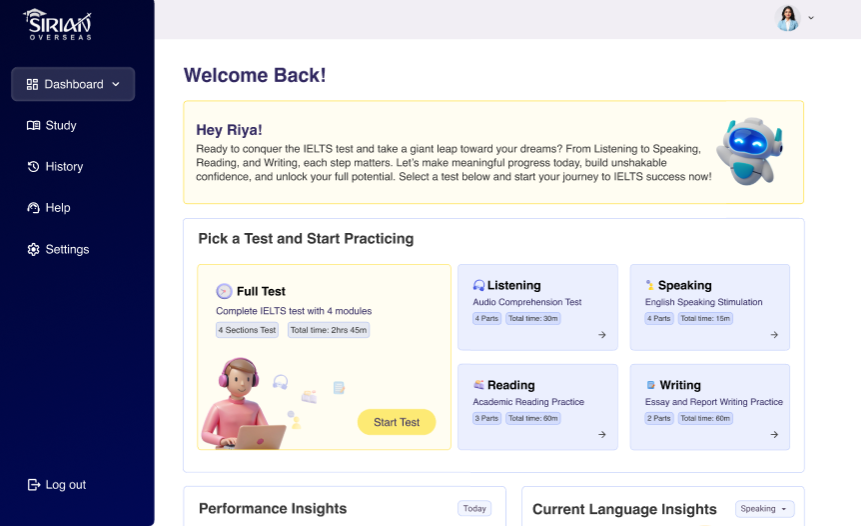
\includegraphics[width=0.8\linewidth]{images/fulltest_dashbaord1.png}
    \caption{Full Test Dashboard}
    \label{fig:fulltest1}
\end{figure}

\begin{figure}[H]
    \centering
    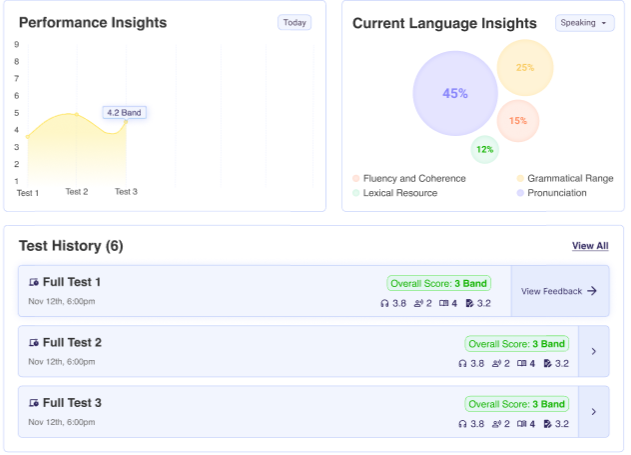
\includegraphics[width=0.8\linewidth]{images/fulltest_dashboard2.png}
    \caption{Full Test Dashboard with History and Metrics}
    \label{fig:fulltest2}
\end{figure}

\vspace{0.5cm}
\subsection{Listening Module Output}
\begin{itemize}
    \item Audio instructions and consent screen verified before test begins.
    \item Timed interface auto-starts audio with questions locked to single-play behavior.
    \item AI-generated feedback confirms accuracy of attempted answers.
\end{itemize}

\begin{figure}[H]
    \centering
    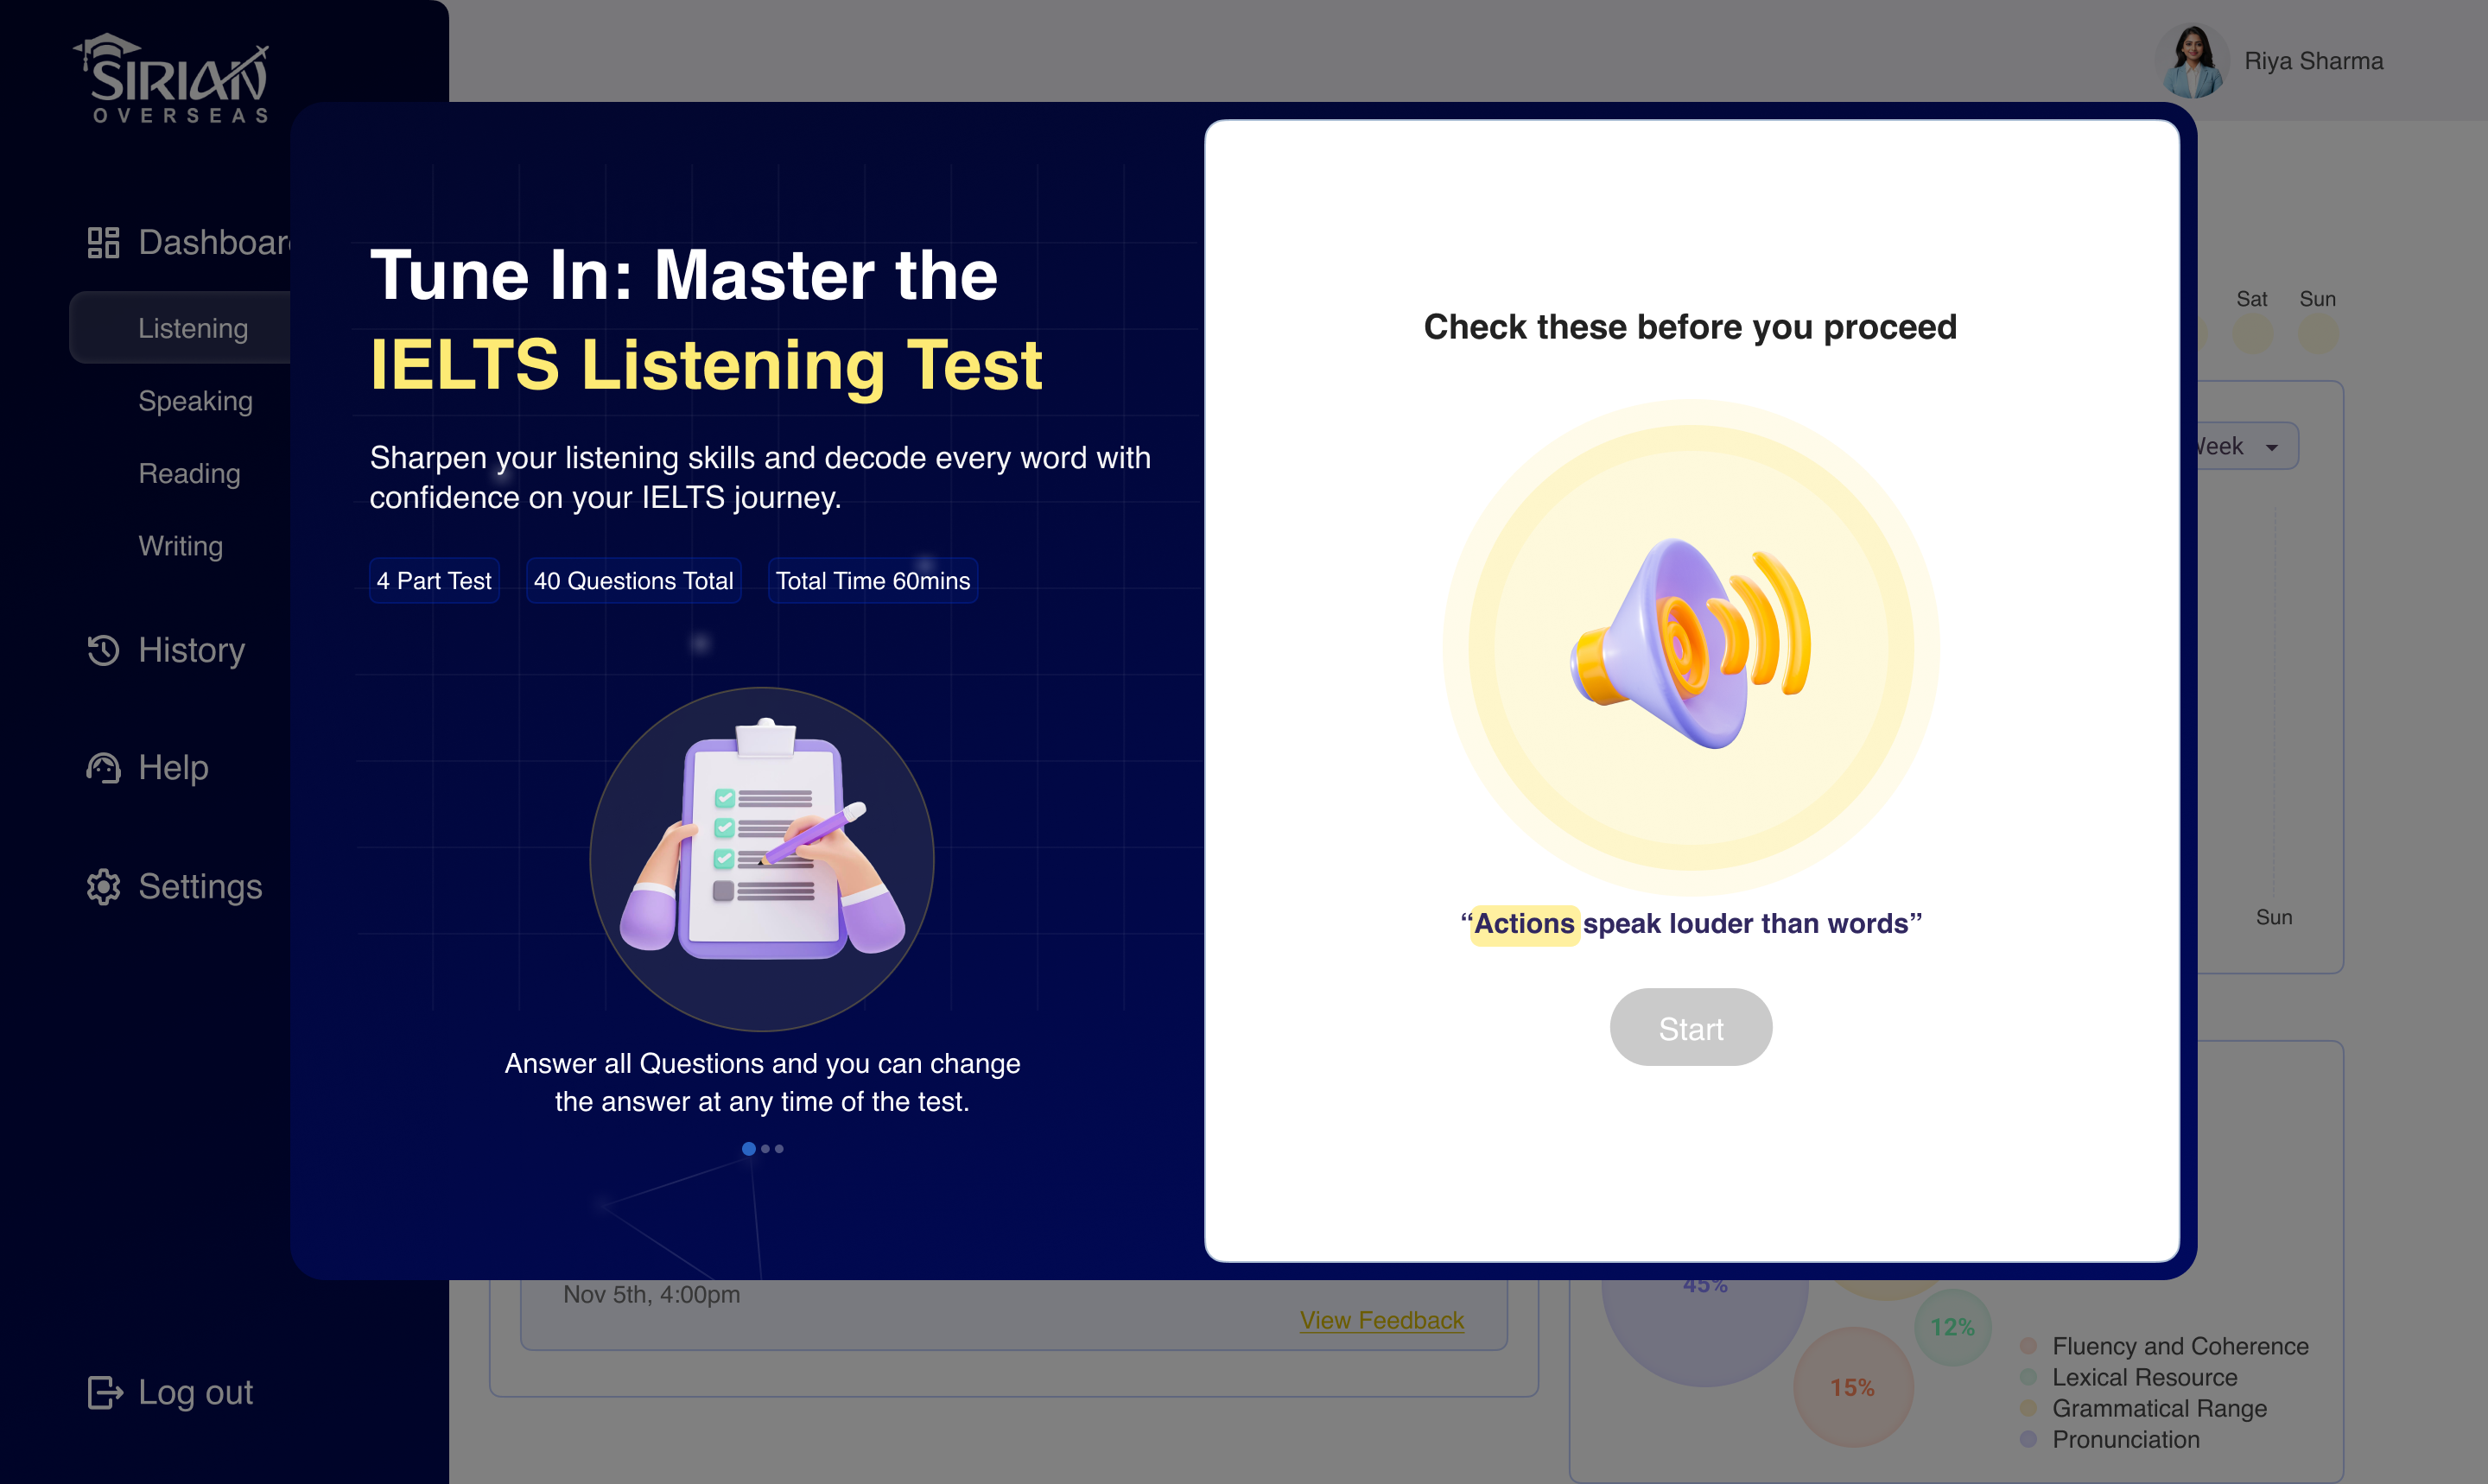
\includegraphics[width=0.8\textwidth]{images/Listening_start_page.png}
    \caption{Listening Module Instruction Screen}
\end{figure}

\begin{figure}[H]
    \centering
    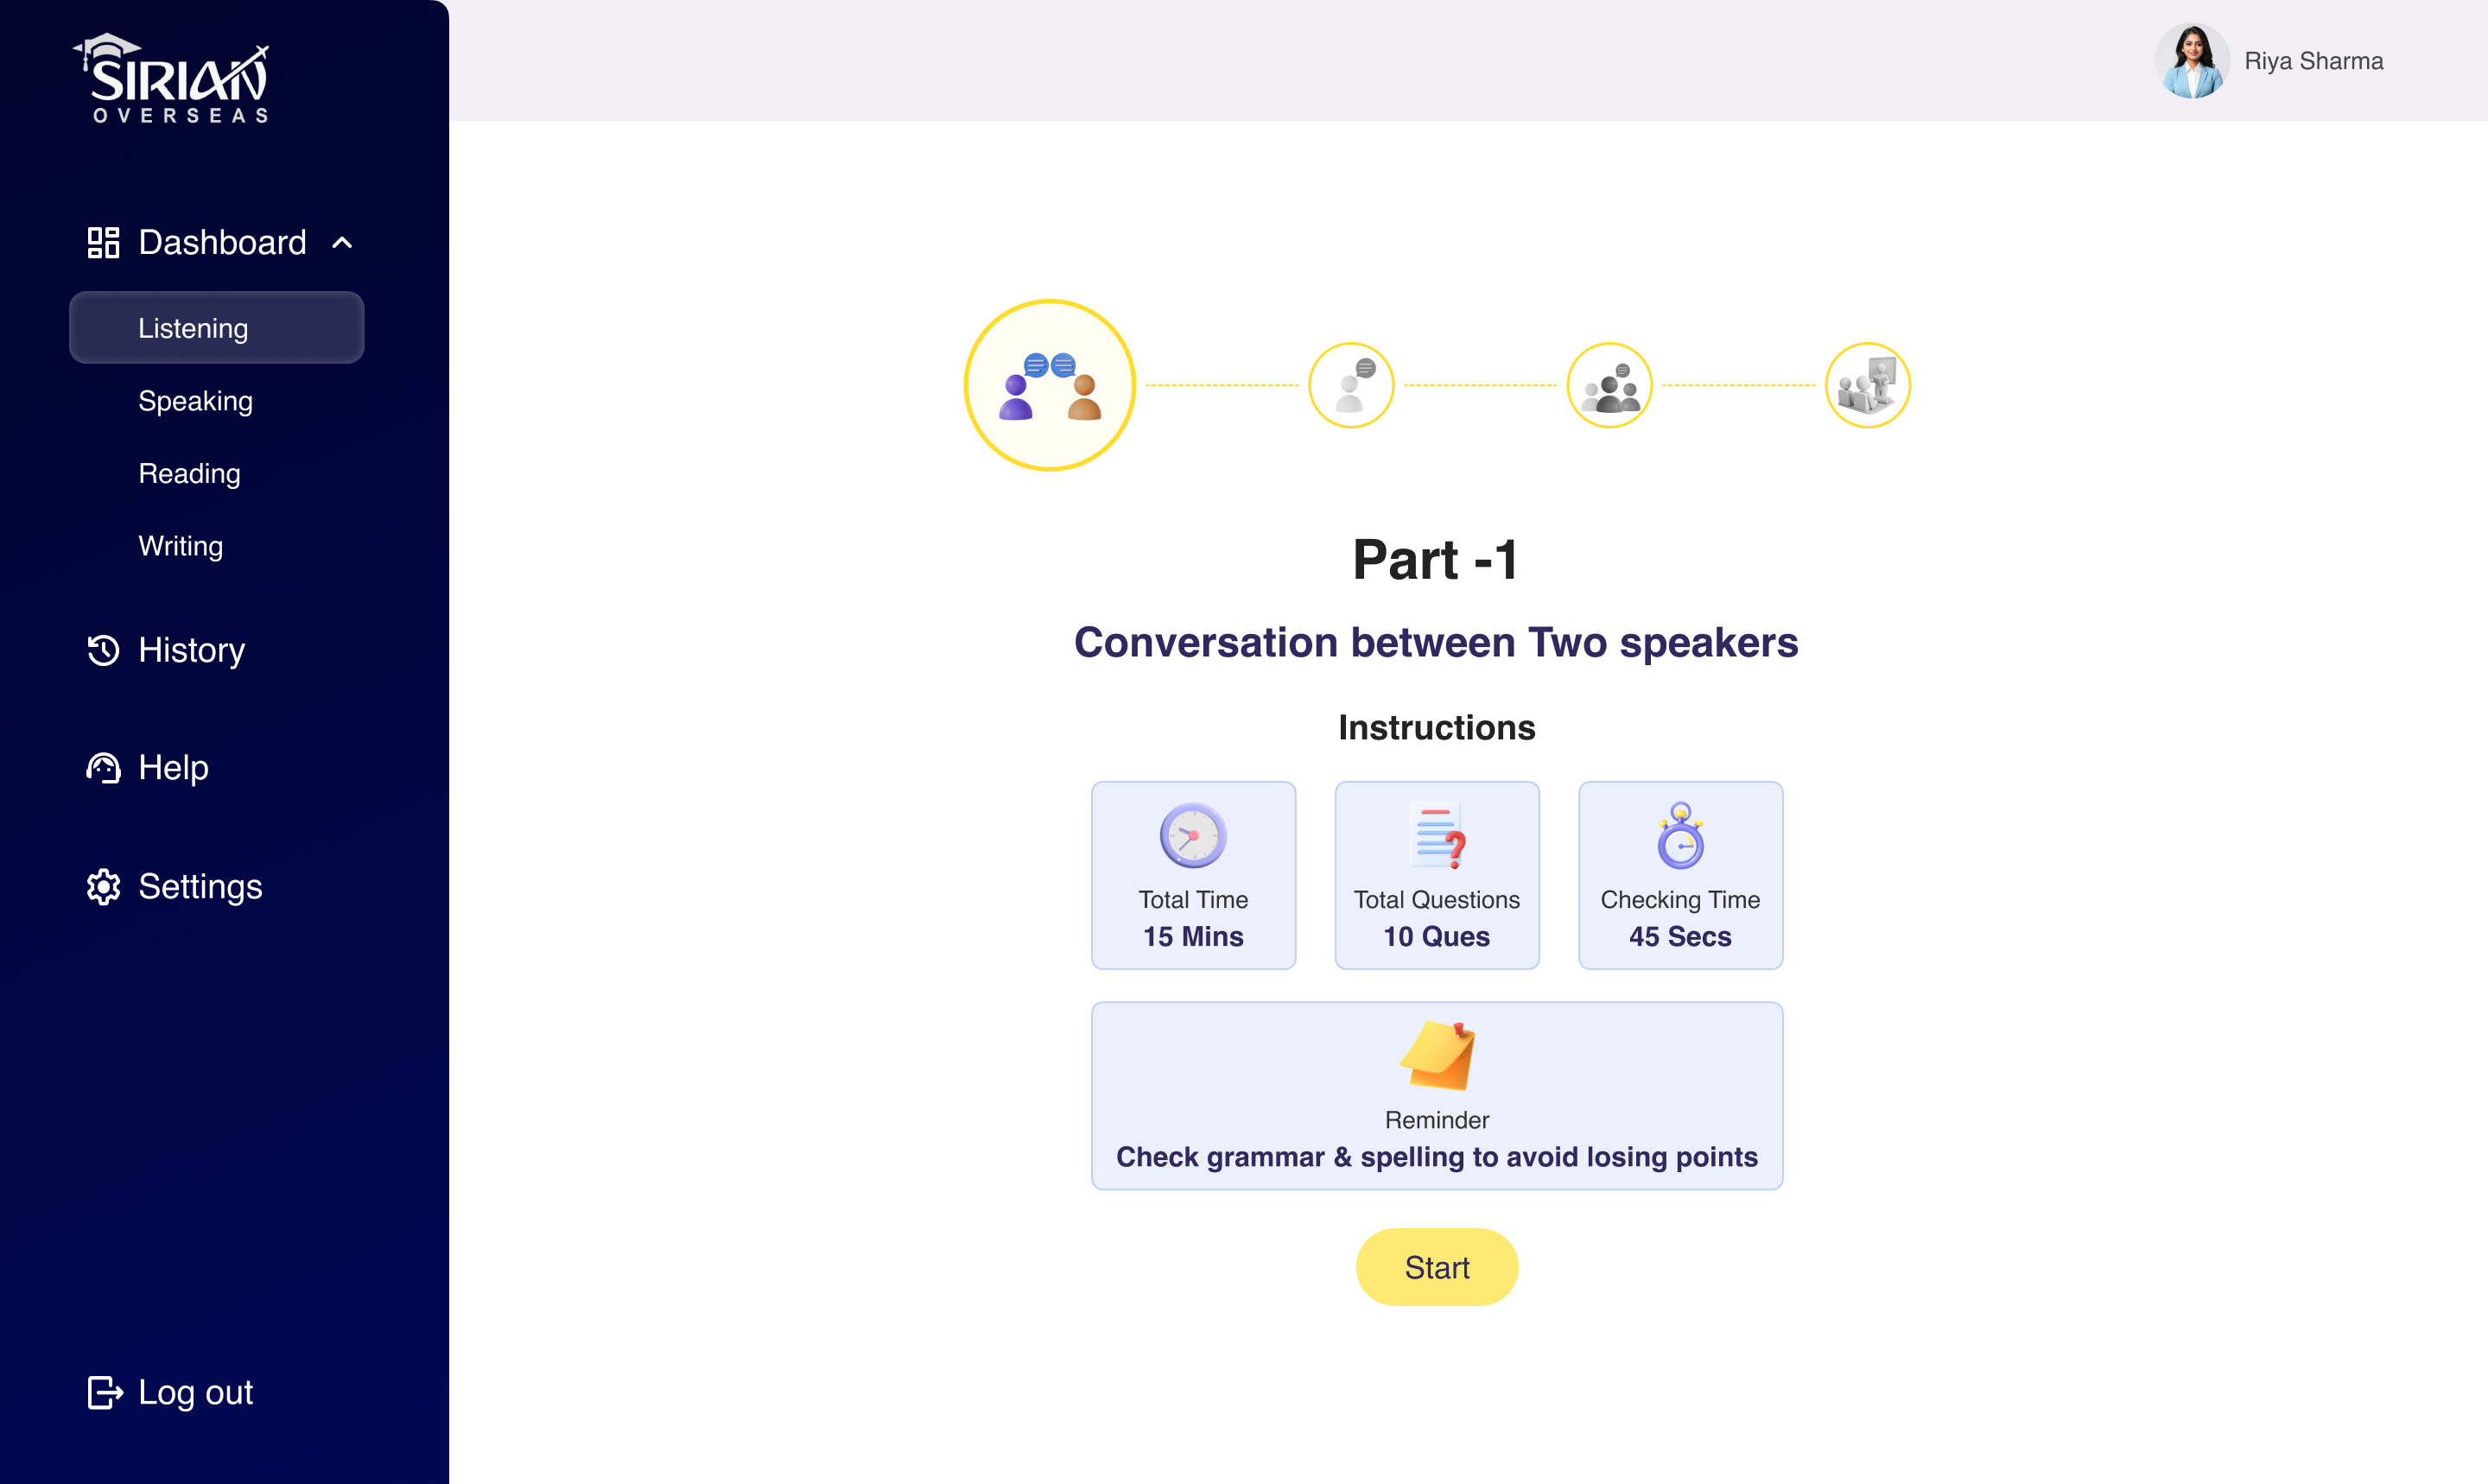
\includegraphics[width=0.8\textwidth]{images/Listening_part1.png}
    \caption{Listening Test Interface with Audio Playback}
\end{figure}

\begin{figure}[H]
    \centering
    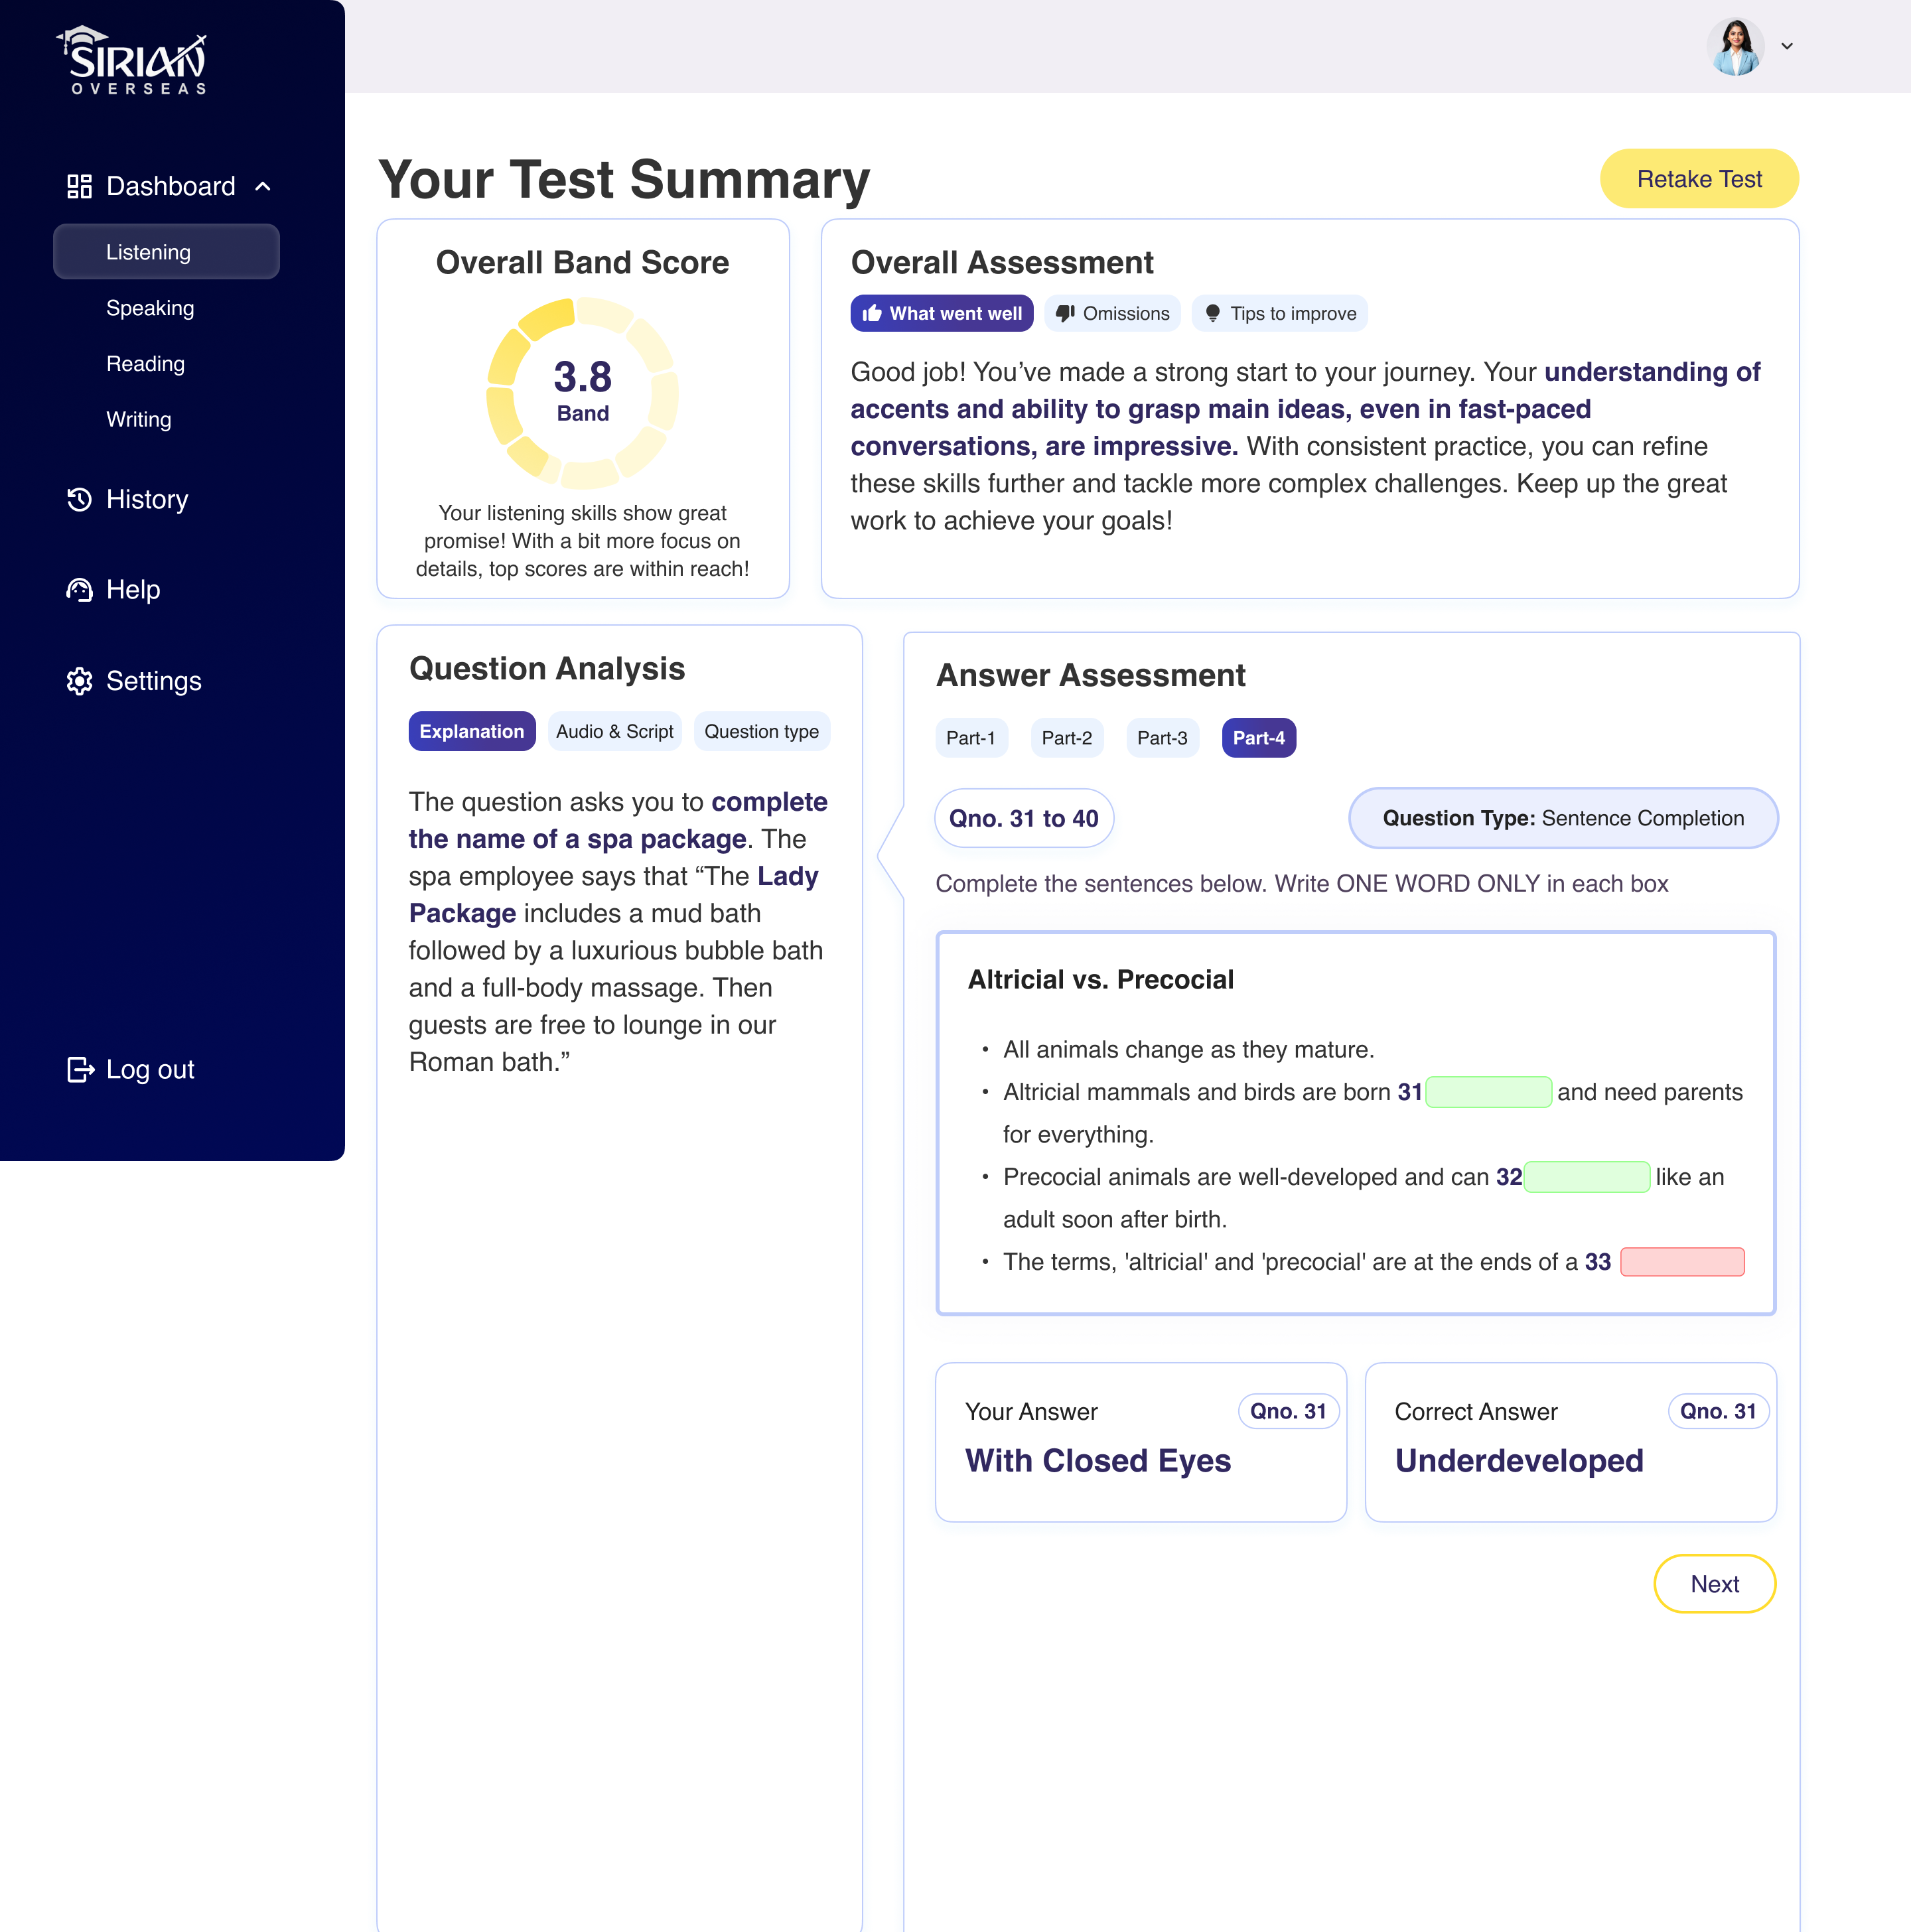
\includegraphics[width=0.8\textwidth]{images/Listening_Feedback_page.png}
    \caption{Listening Module Feedback and Score}
\end{figure}

\vspace{0.3cm}
\subsection{Reading Module Output}
\begin{itemize}
    \item Passage-based questions dynamically loaded.
    \item Timed interface with scrollable paragraphs and question sections.
    \item Visual indicators and answer tracking validated.
\end{itemize}

\begin{figure}[H]
    \centering
    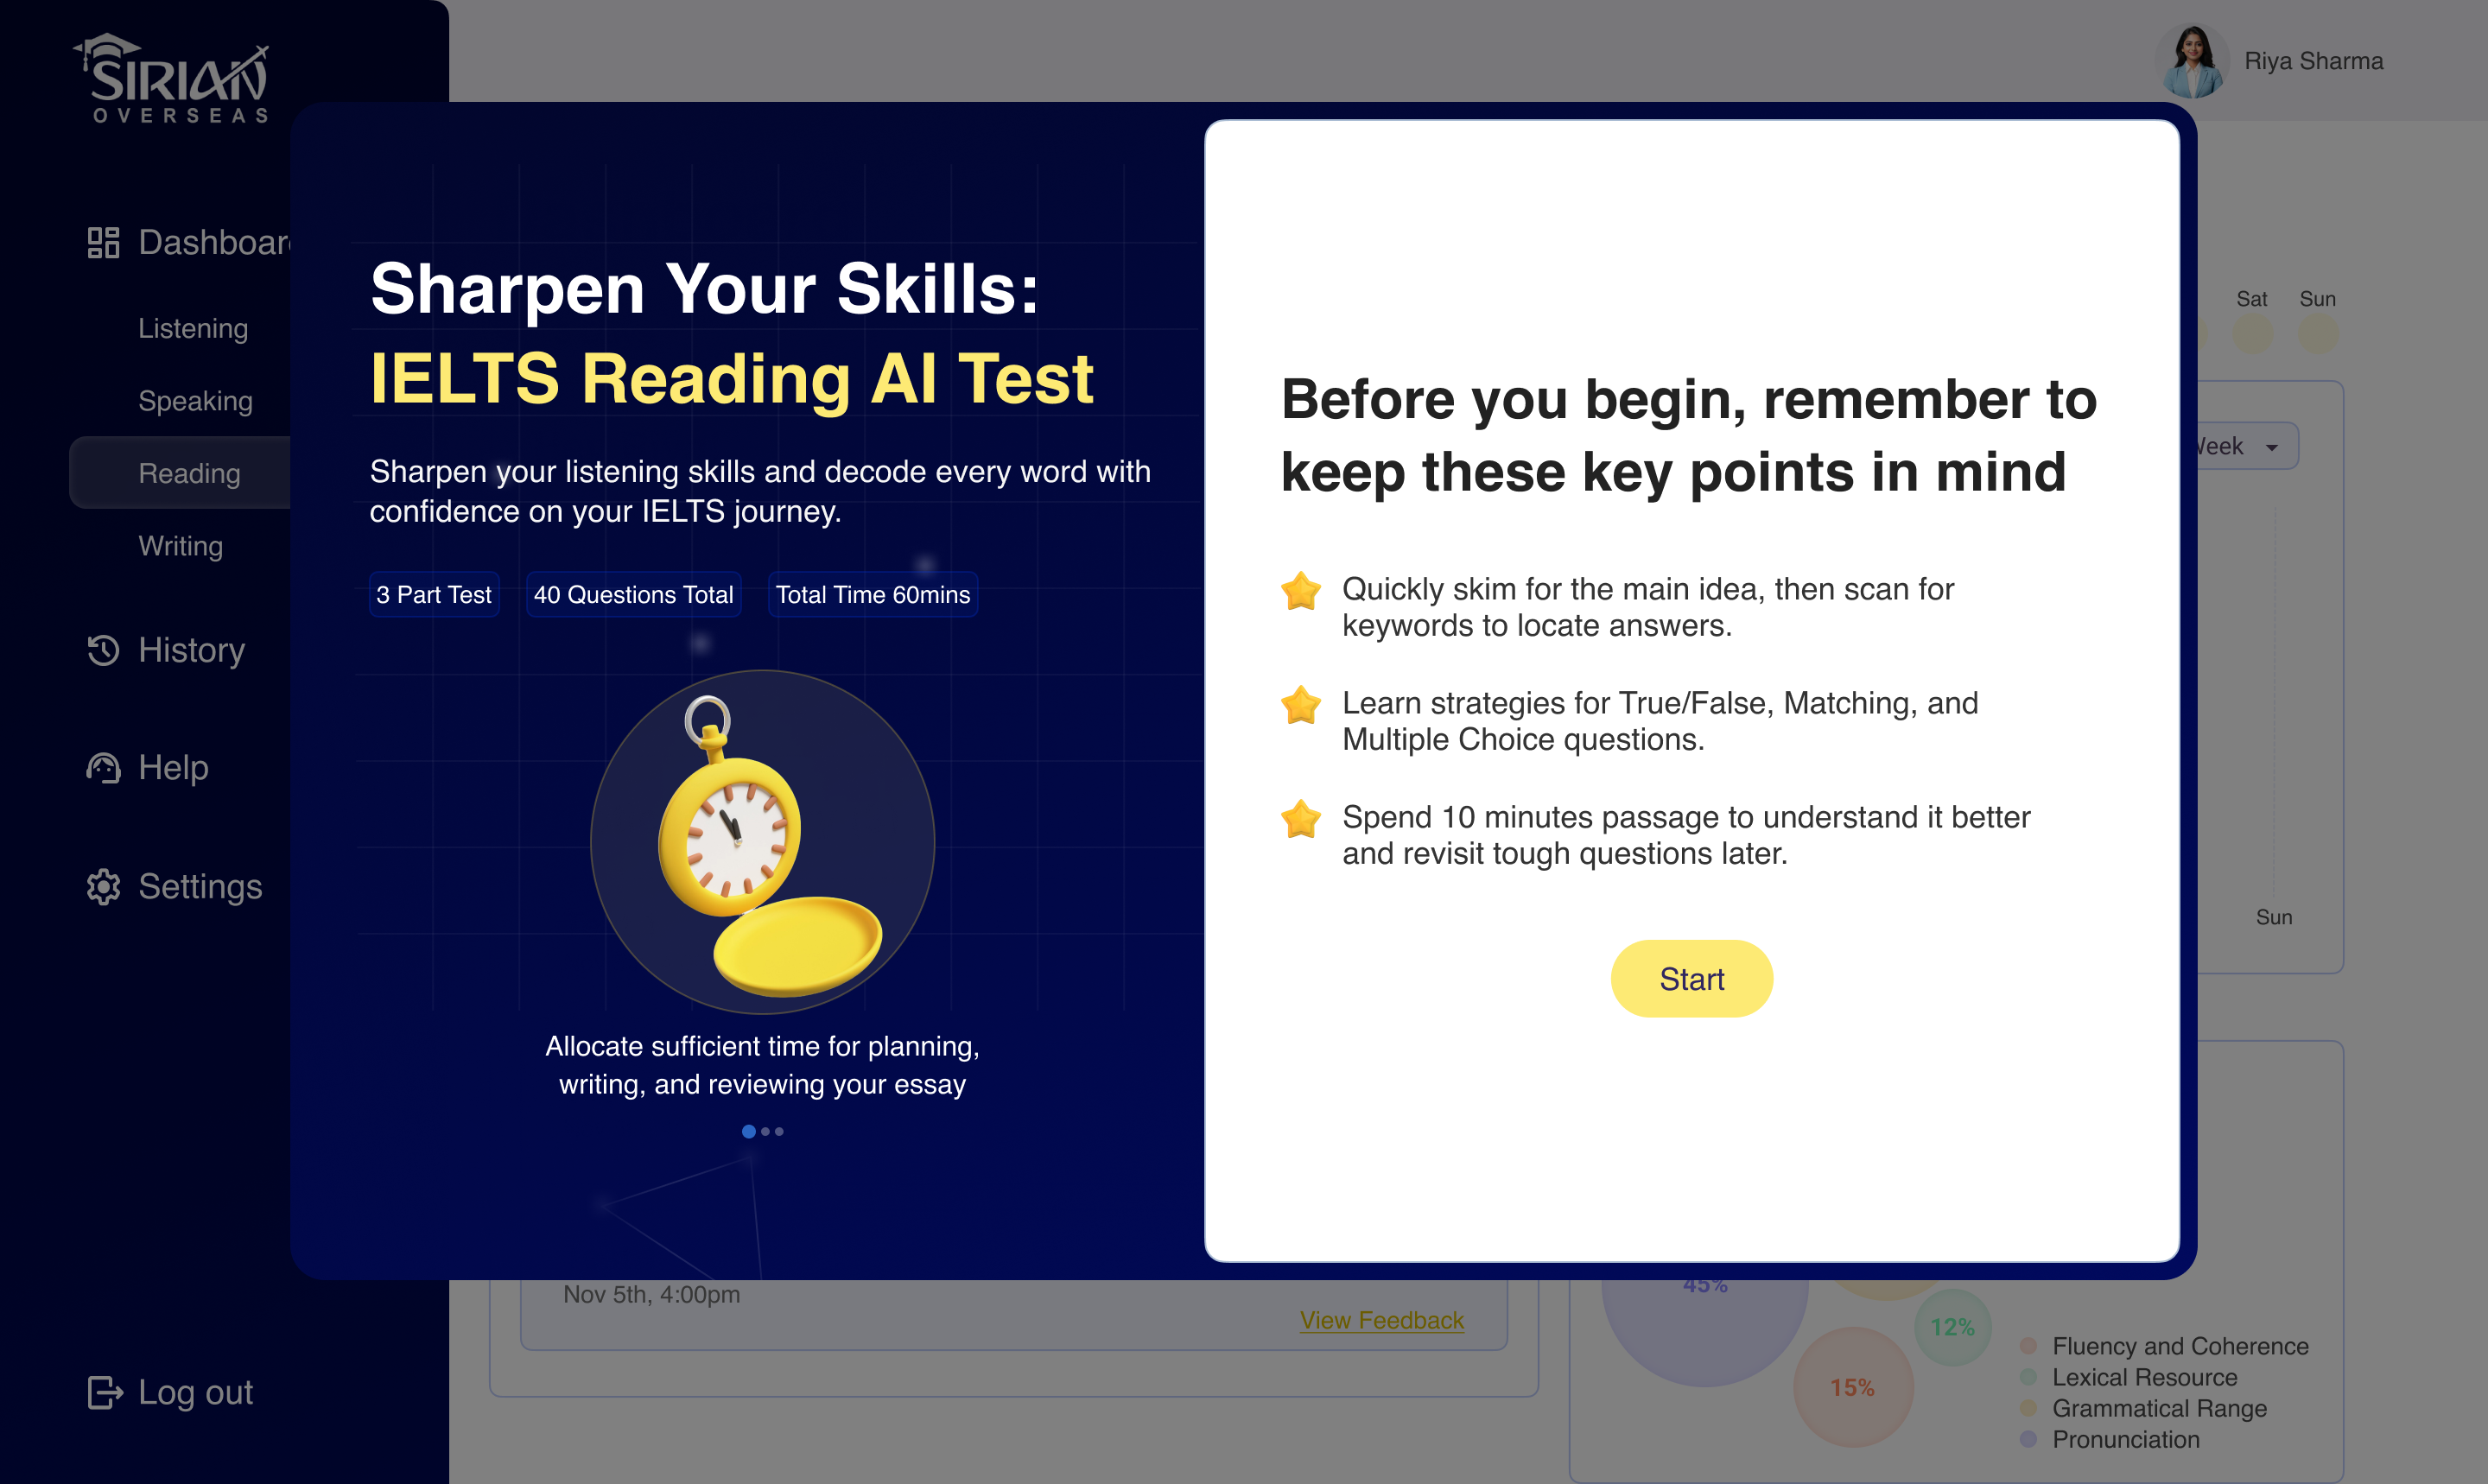
\includegraphics[width=0.8\textwidth]{images/Reading_start_page.png}
    \caption{Reading Instructions and Test Overview}
\end{figure}

\begin{figure}[H]
    \centering
    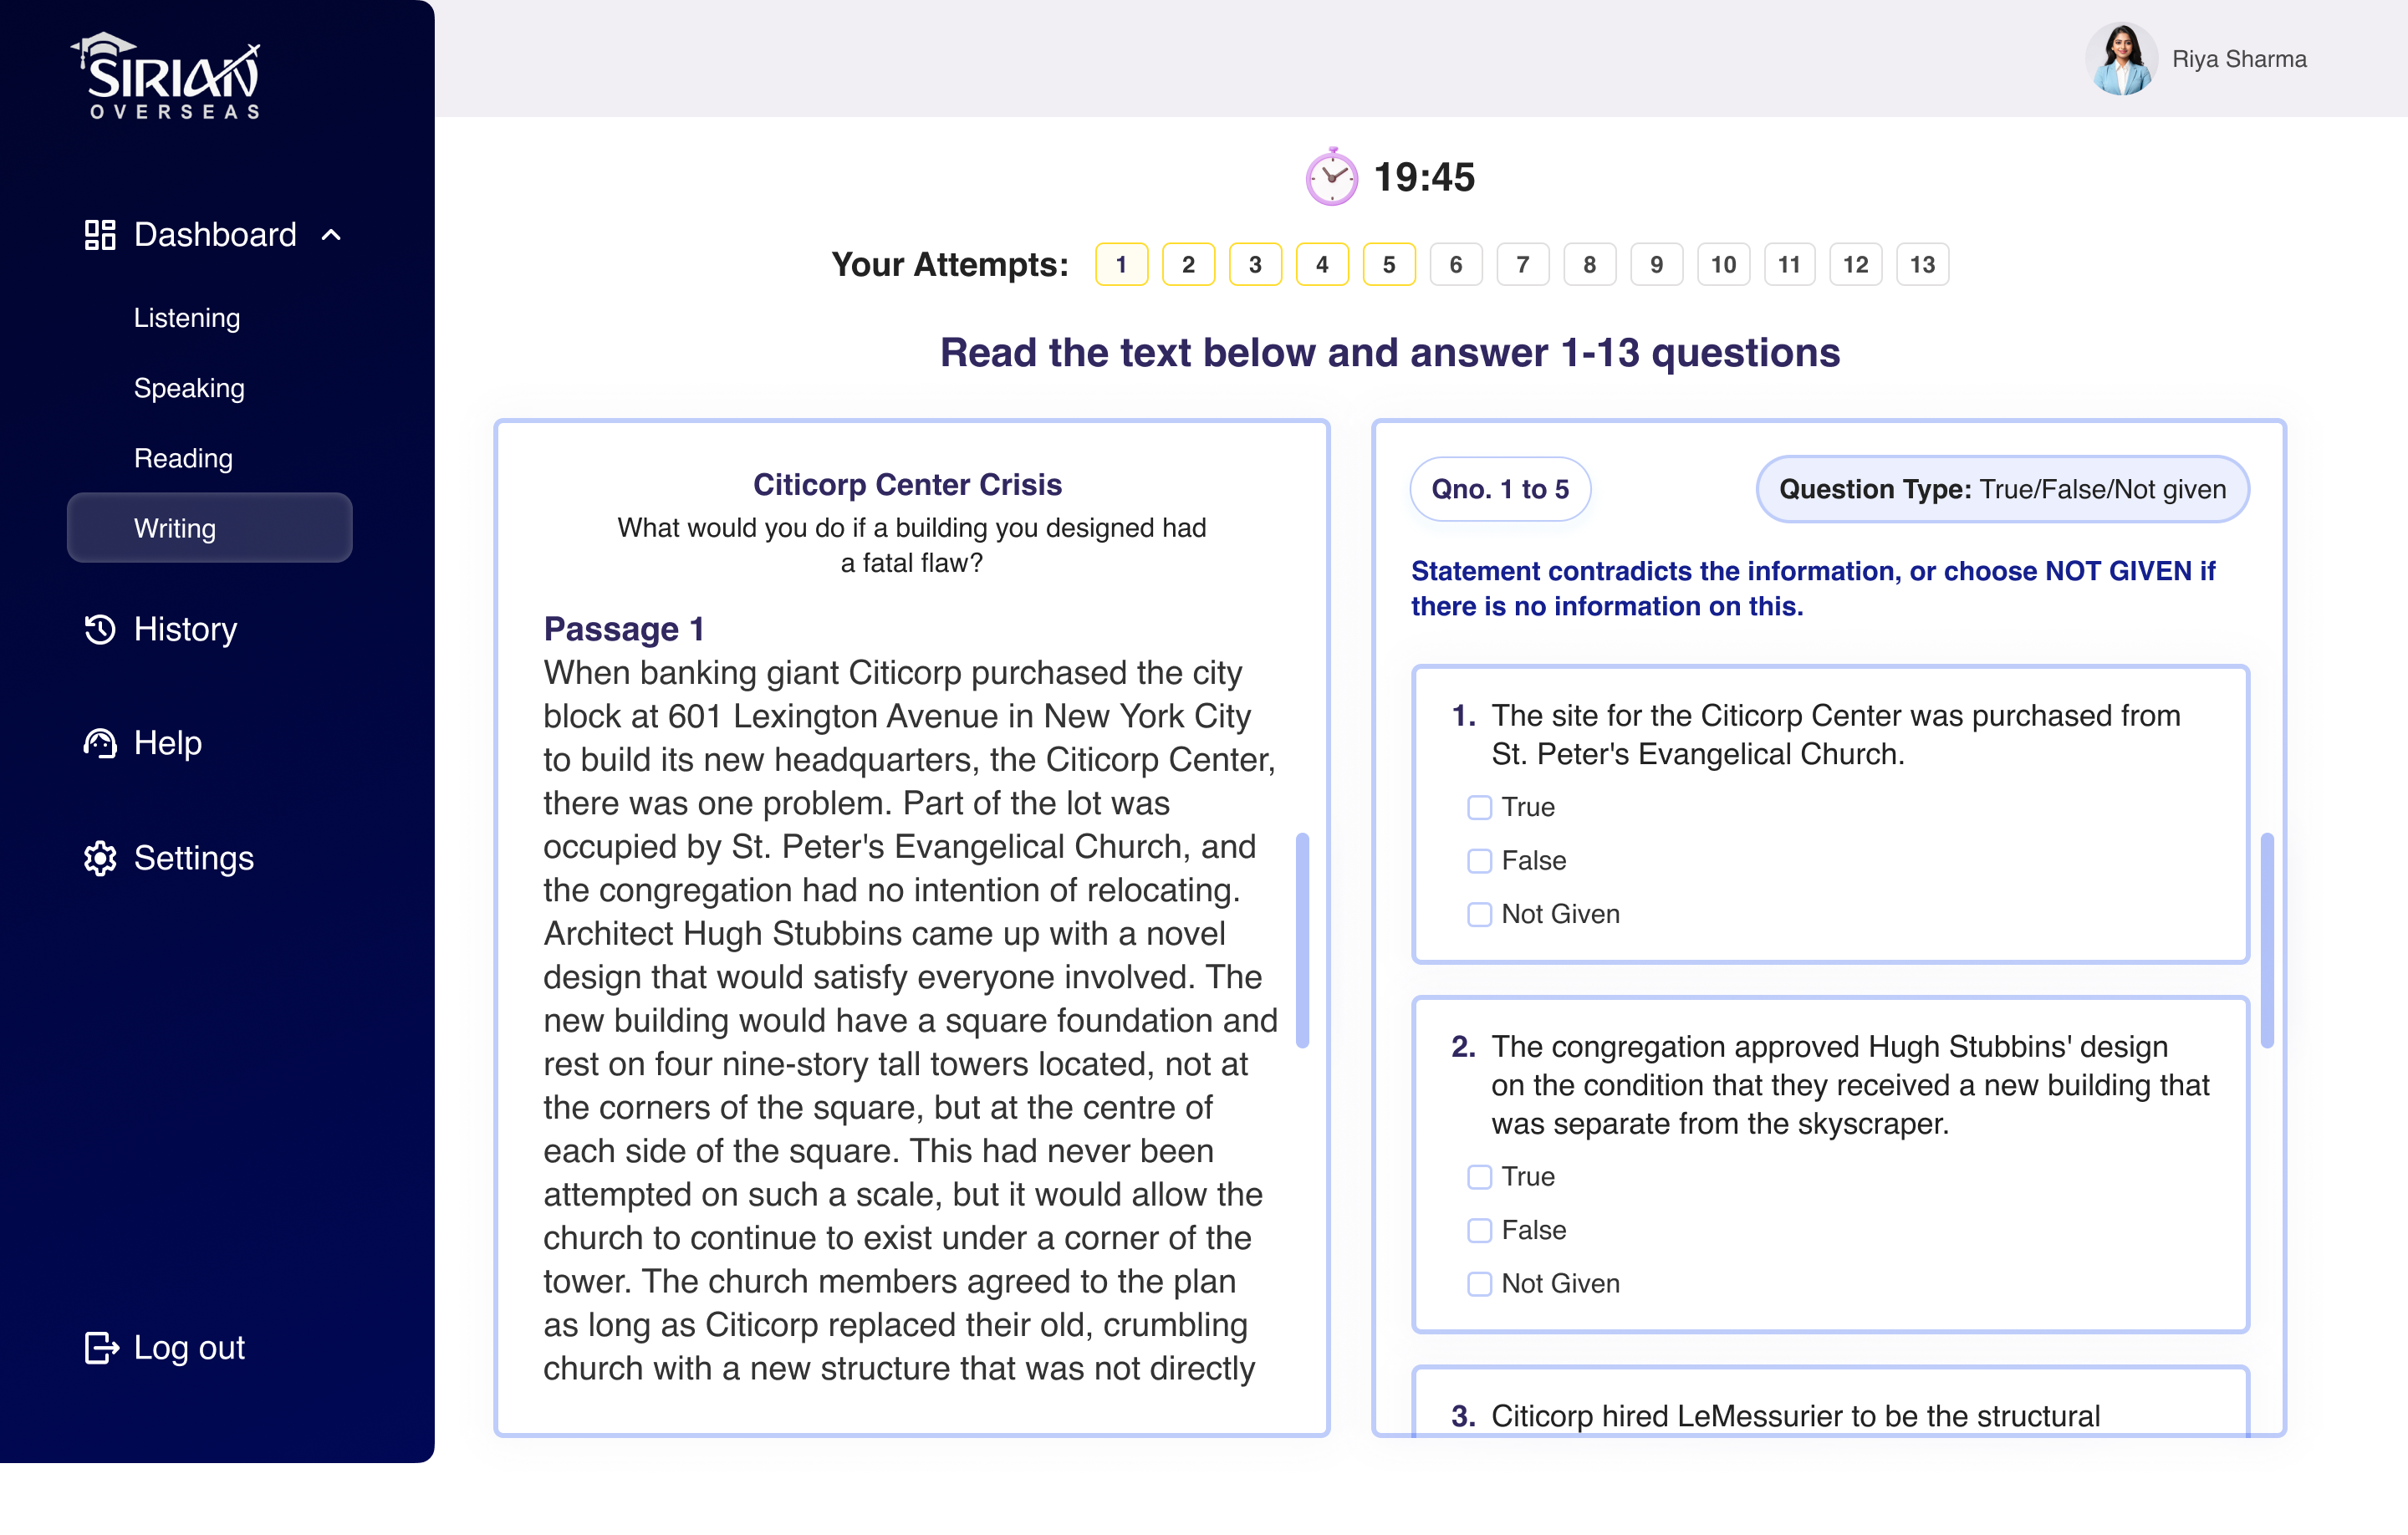
\includegraphics[width=0.8\textwidth]{images/Reading_exam_interface.png}
    \caption{Reading Test Interface with MCQs and Timer}
\end{figure}

\begin{figure}[H]
    \centering
    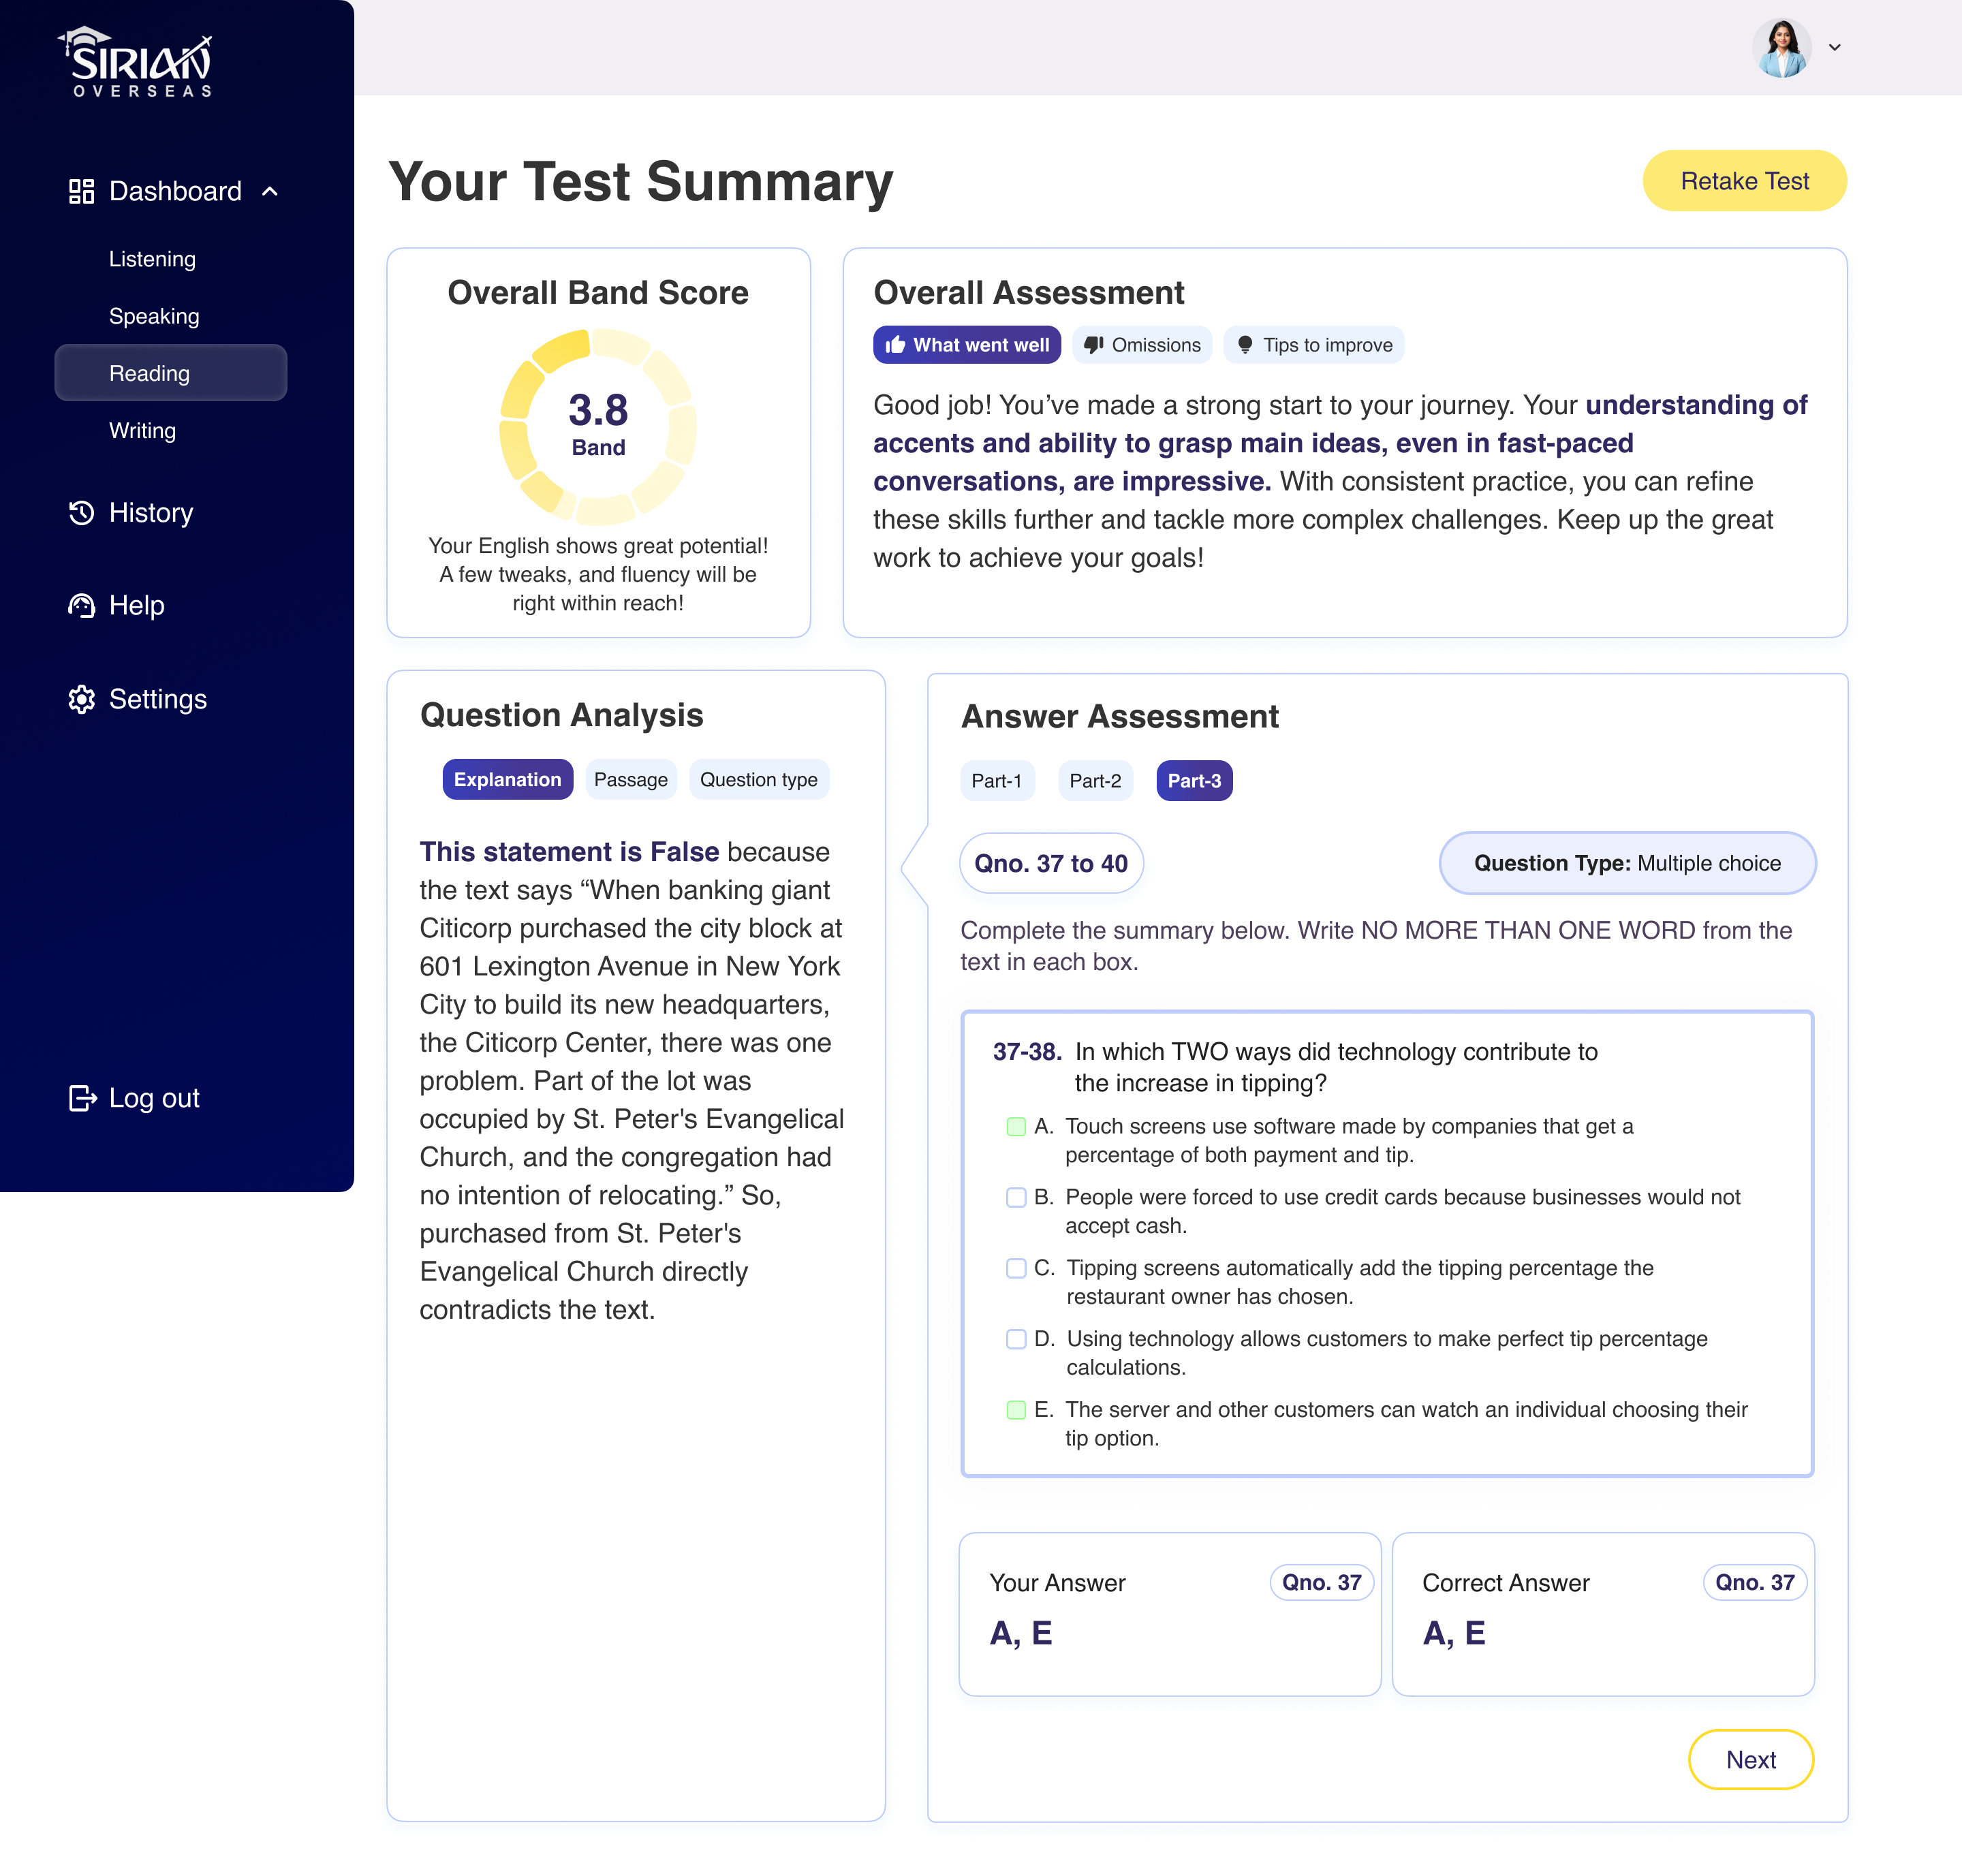
\includegraphics[width=0.8\textwidth]{images/Reading_feedback_page.png}
    \caption{Reading Feedback Section with Correct Answers}
\end{figure}

\vspace{0.3cm}
\subsection{Writing Module Output}
\begin{itemize}
    \item Both Task 1 (Report) and Task 2 (Essay) implemented with minimum word checks.
    \item Timer-based restriction for each section (20 min + 40 min).
    \item AI feedback generated using OpenAI API for grammar and coherence.
\end{itemize}

\begin{figure}[H]
    \centering
    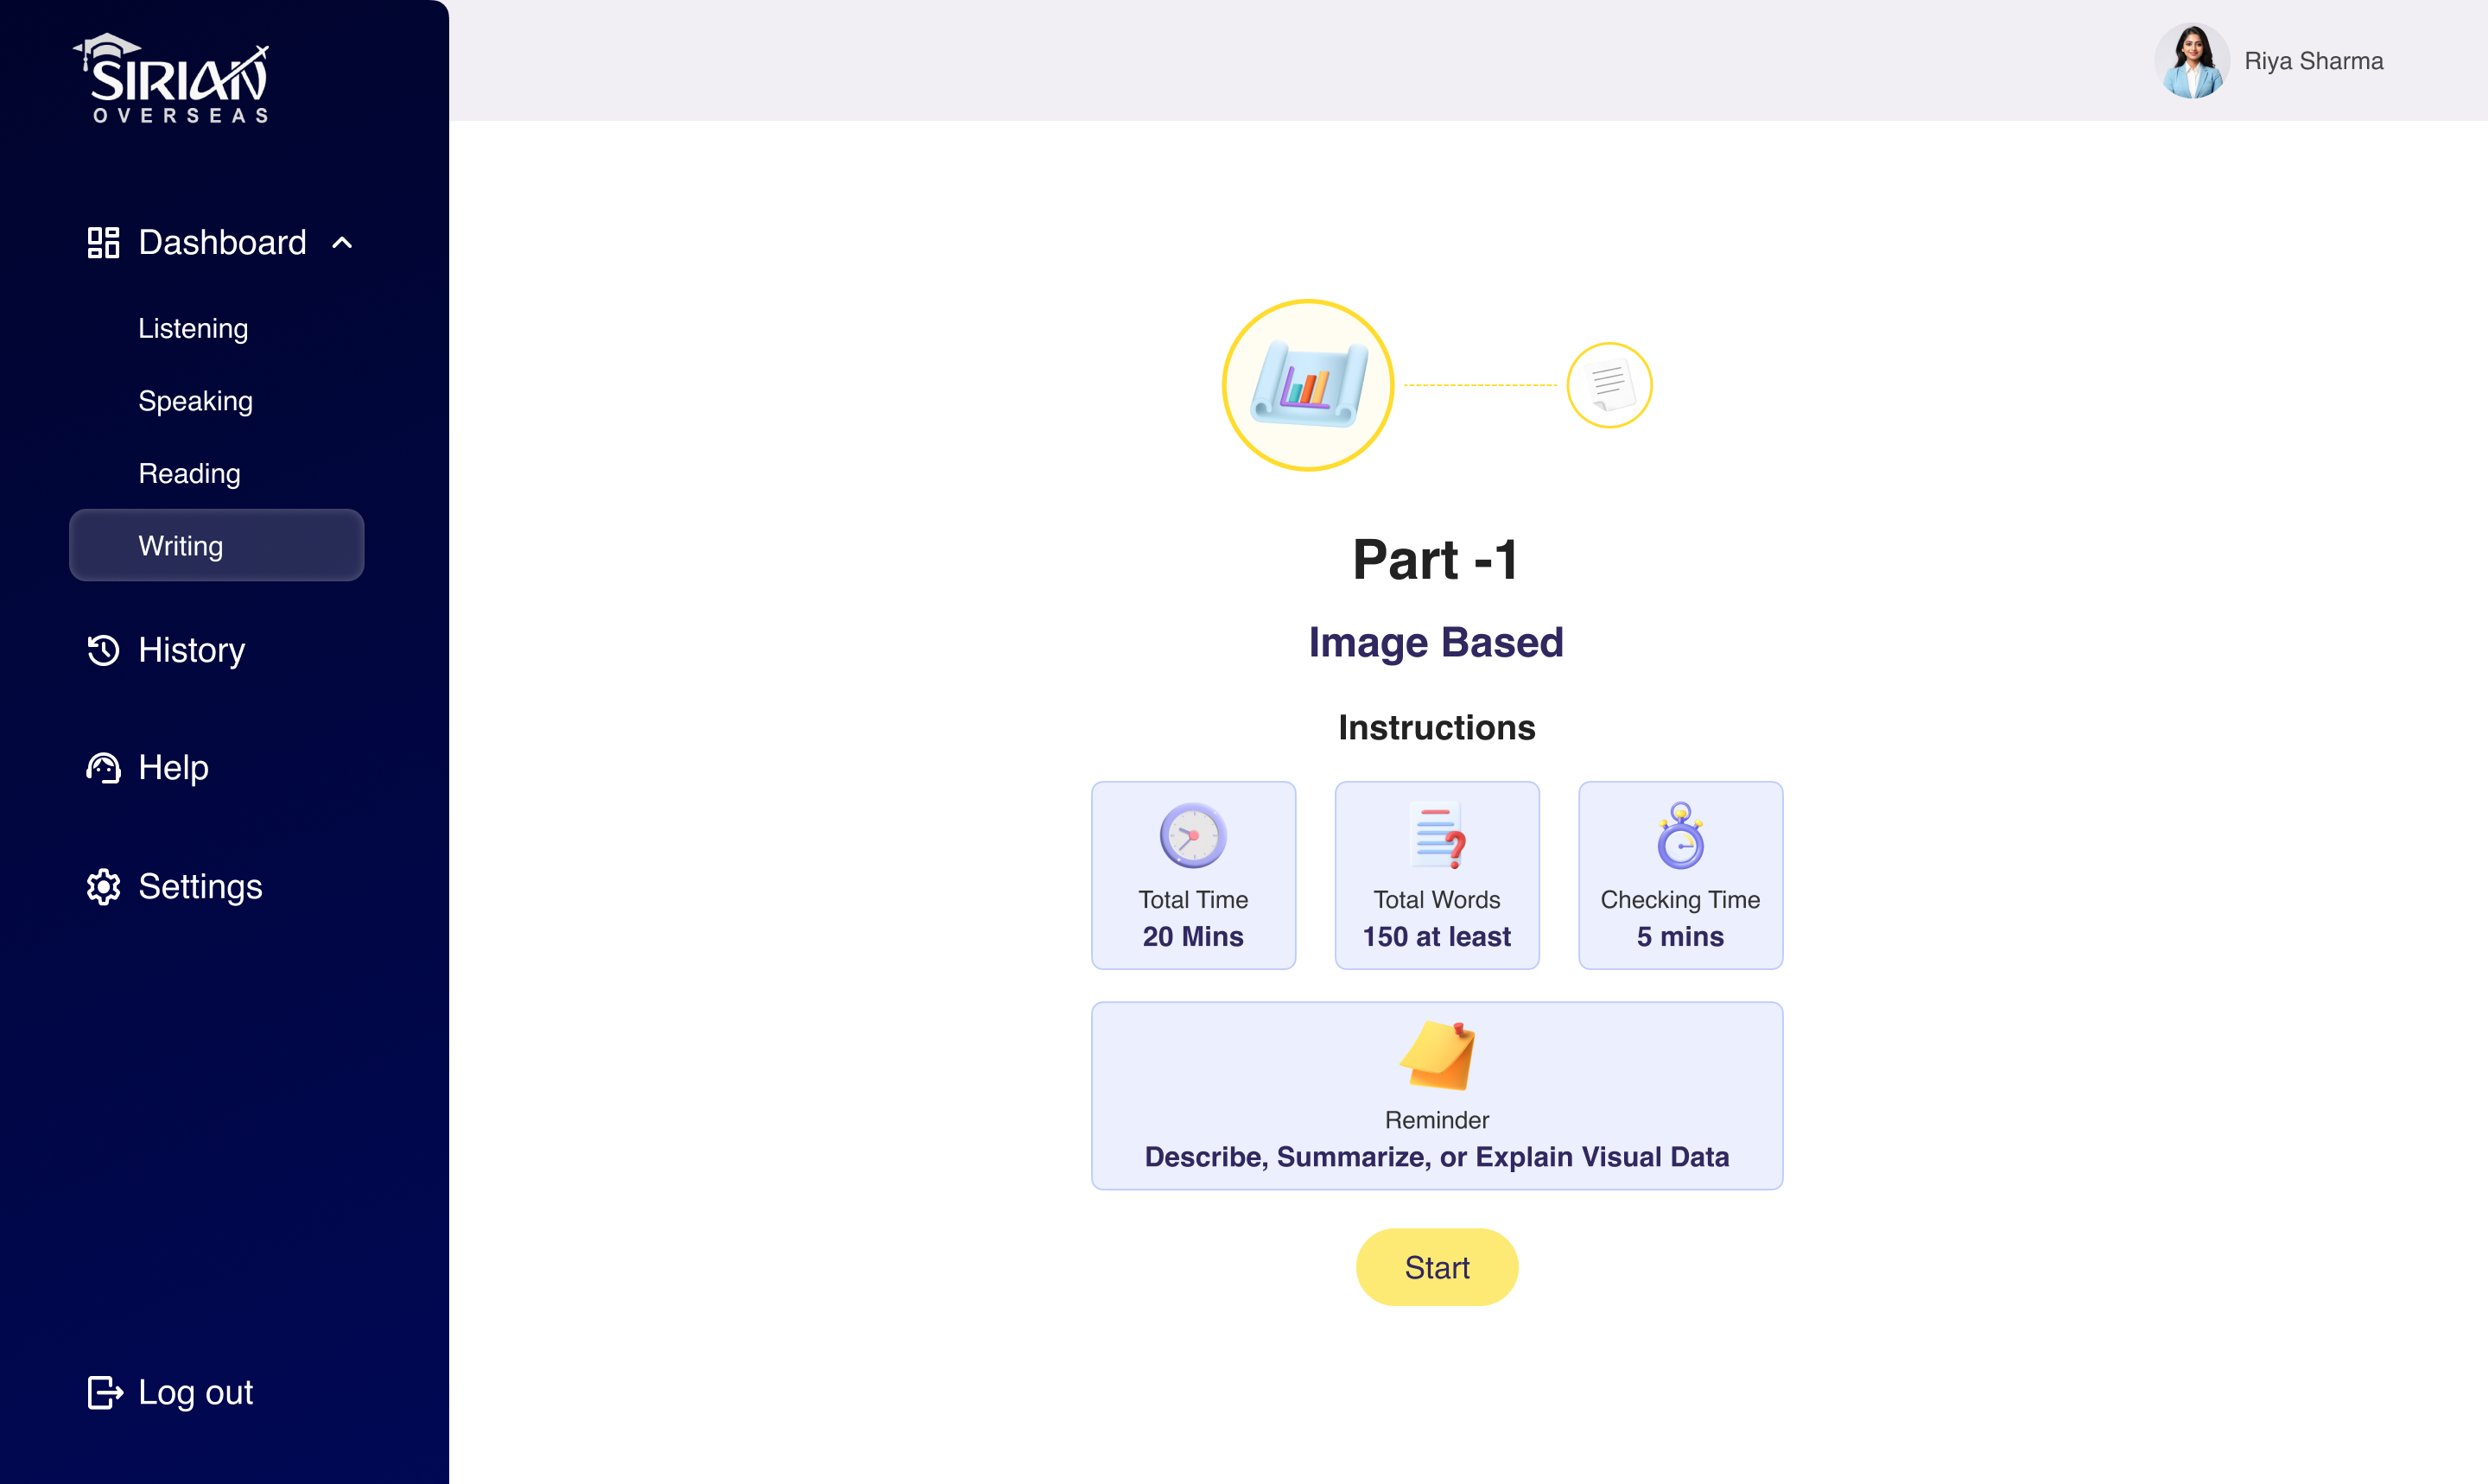
\includegraphics[width=0.8\textwidth]{images/Writing_exam_interface.png}
    \caption{Writing Tasks Interface}
\end{figure}

\begin{figure}[H]
    \centering
    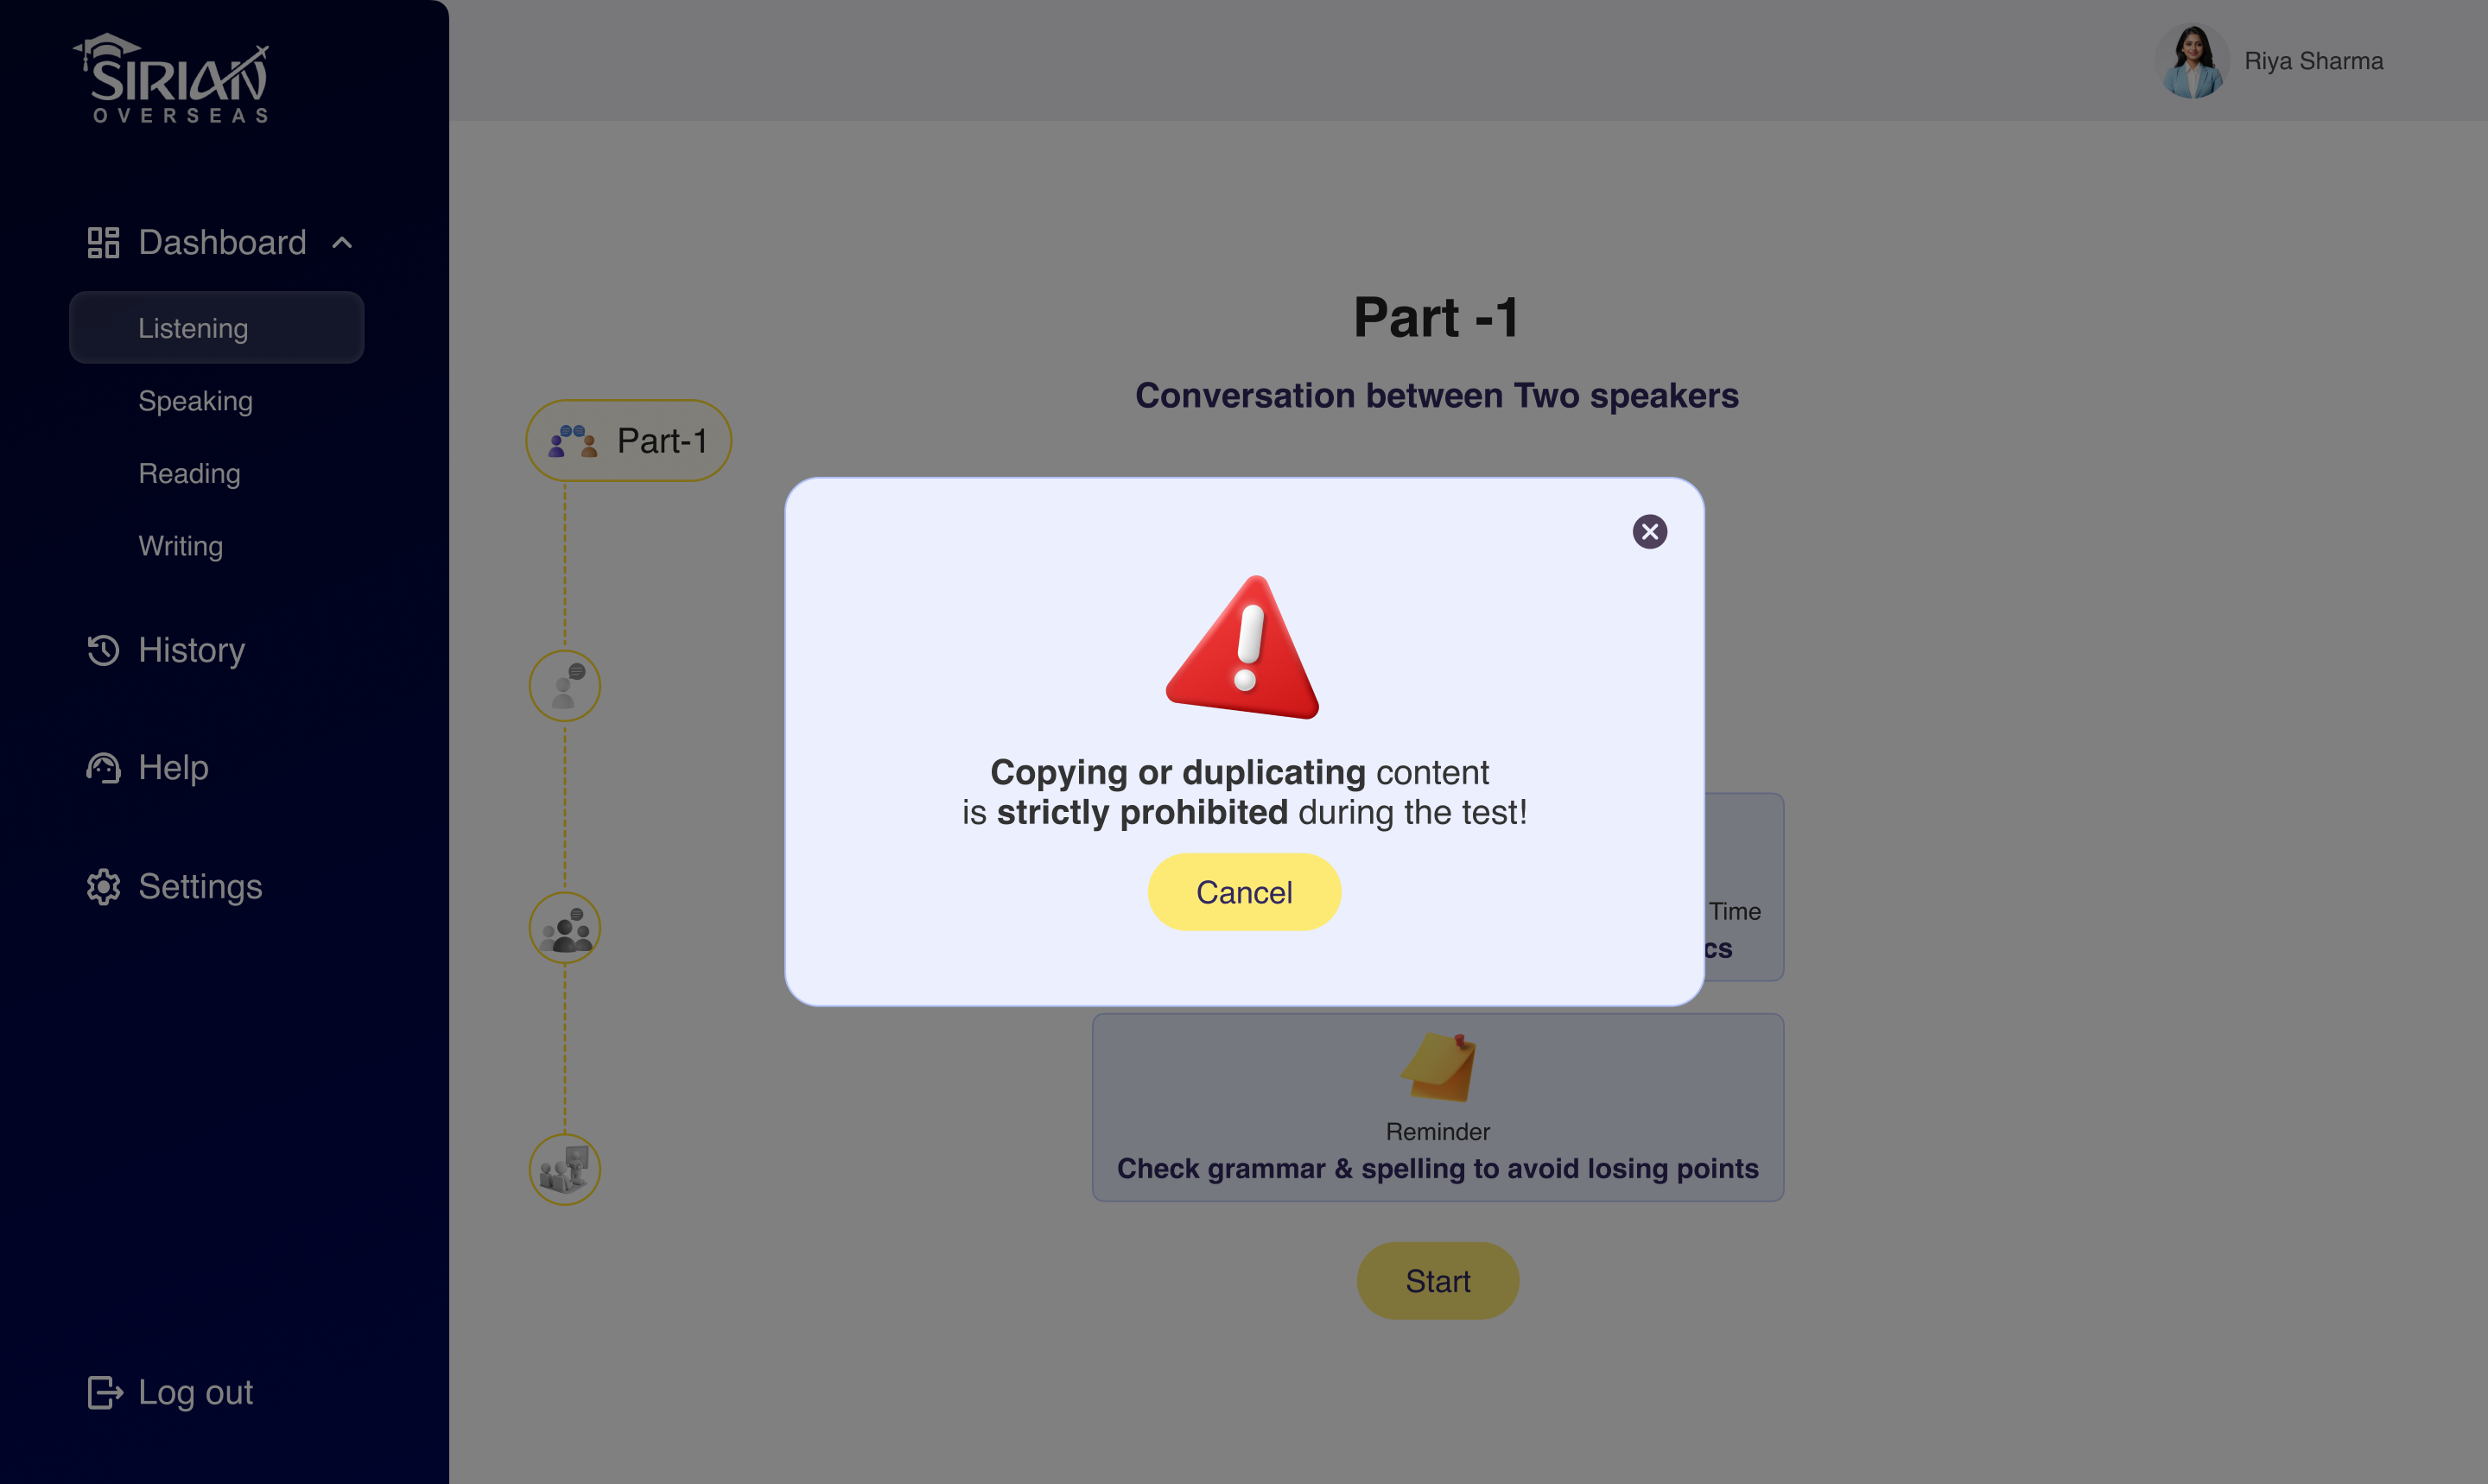
\includegraphics[width=0.8\textwidth]{images/Writing_CopyWarning_page.png}
    \caption{Writing Test Interface with Warning Message on COPY text}
\end{figure}

\begin{figure}[H]
    \centering
    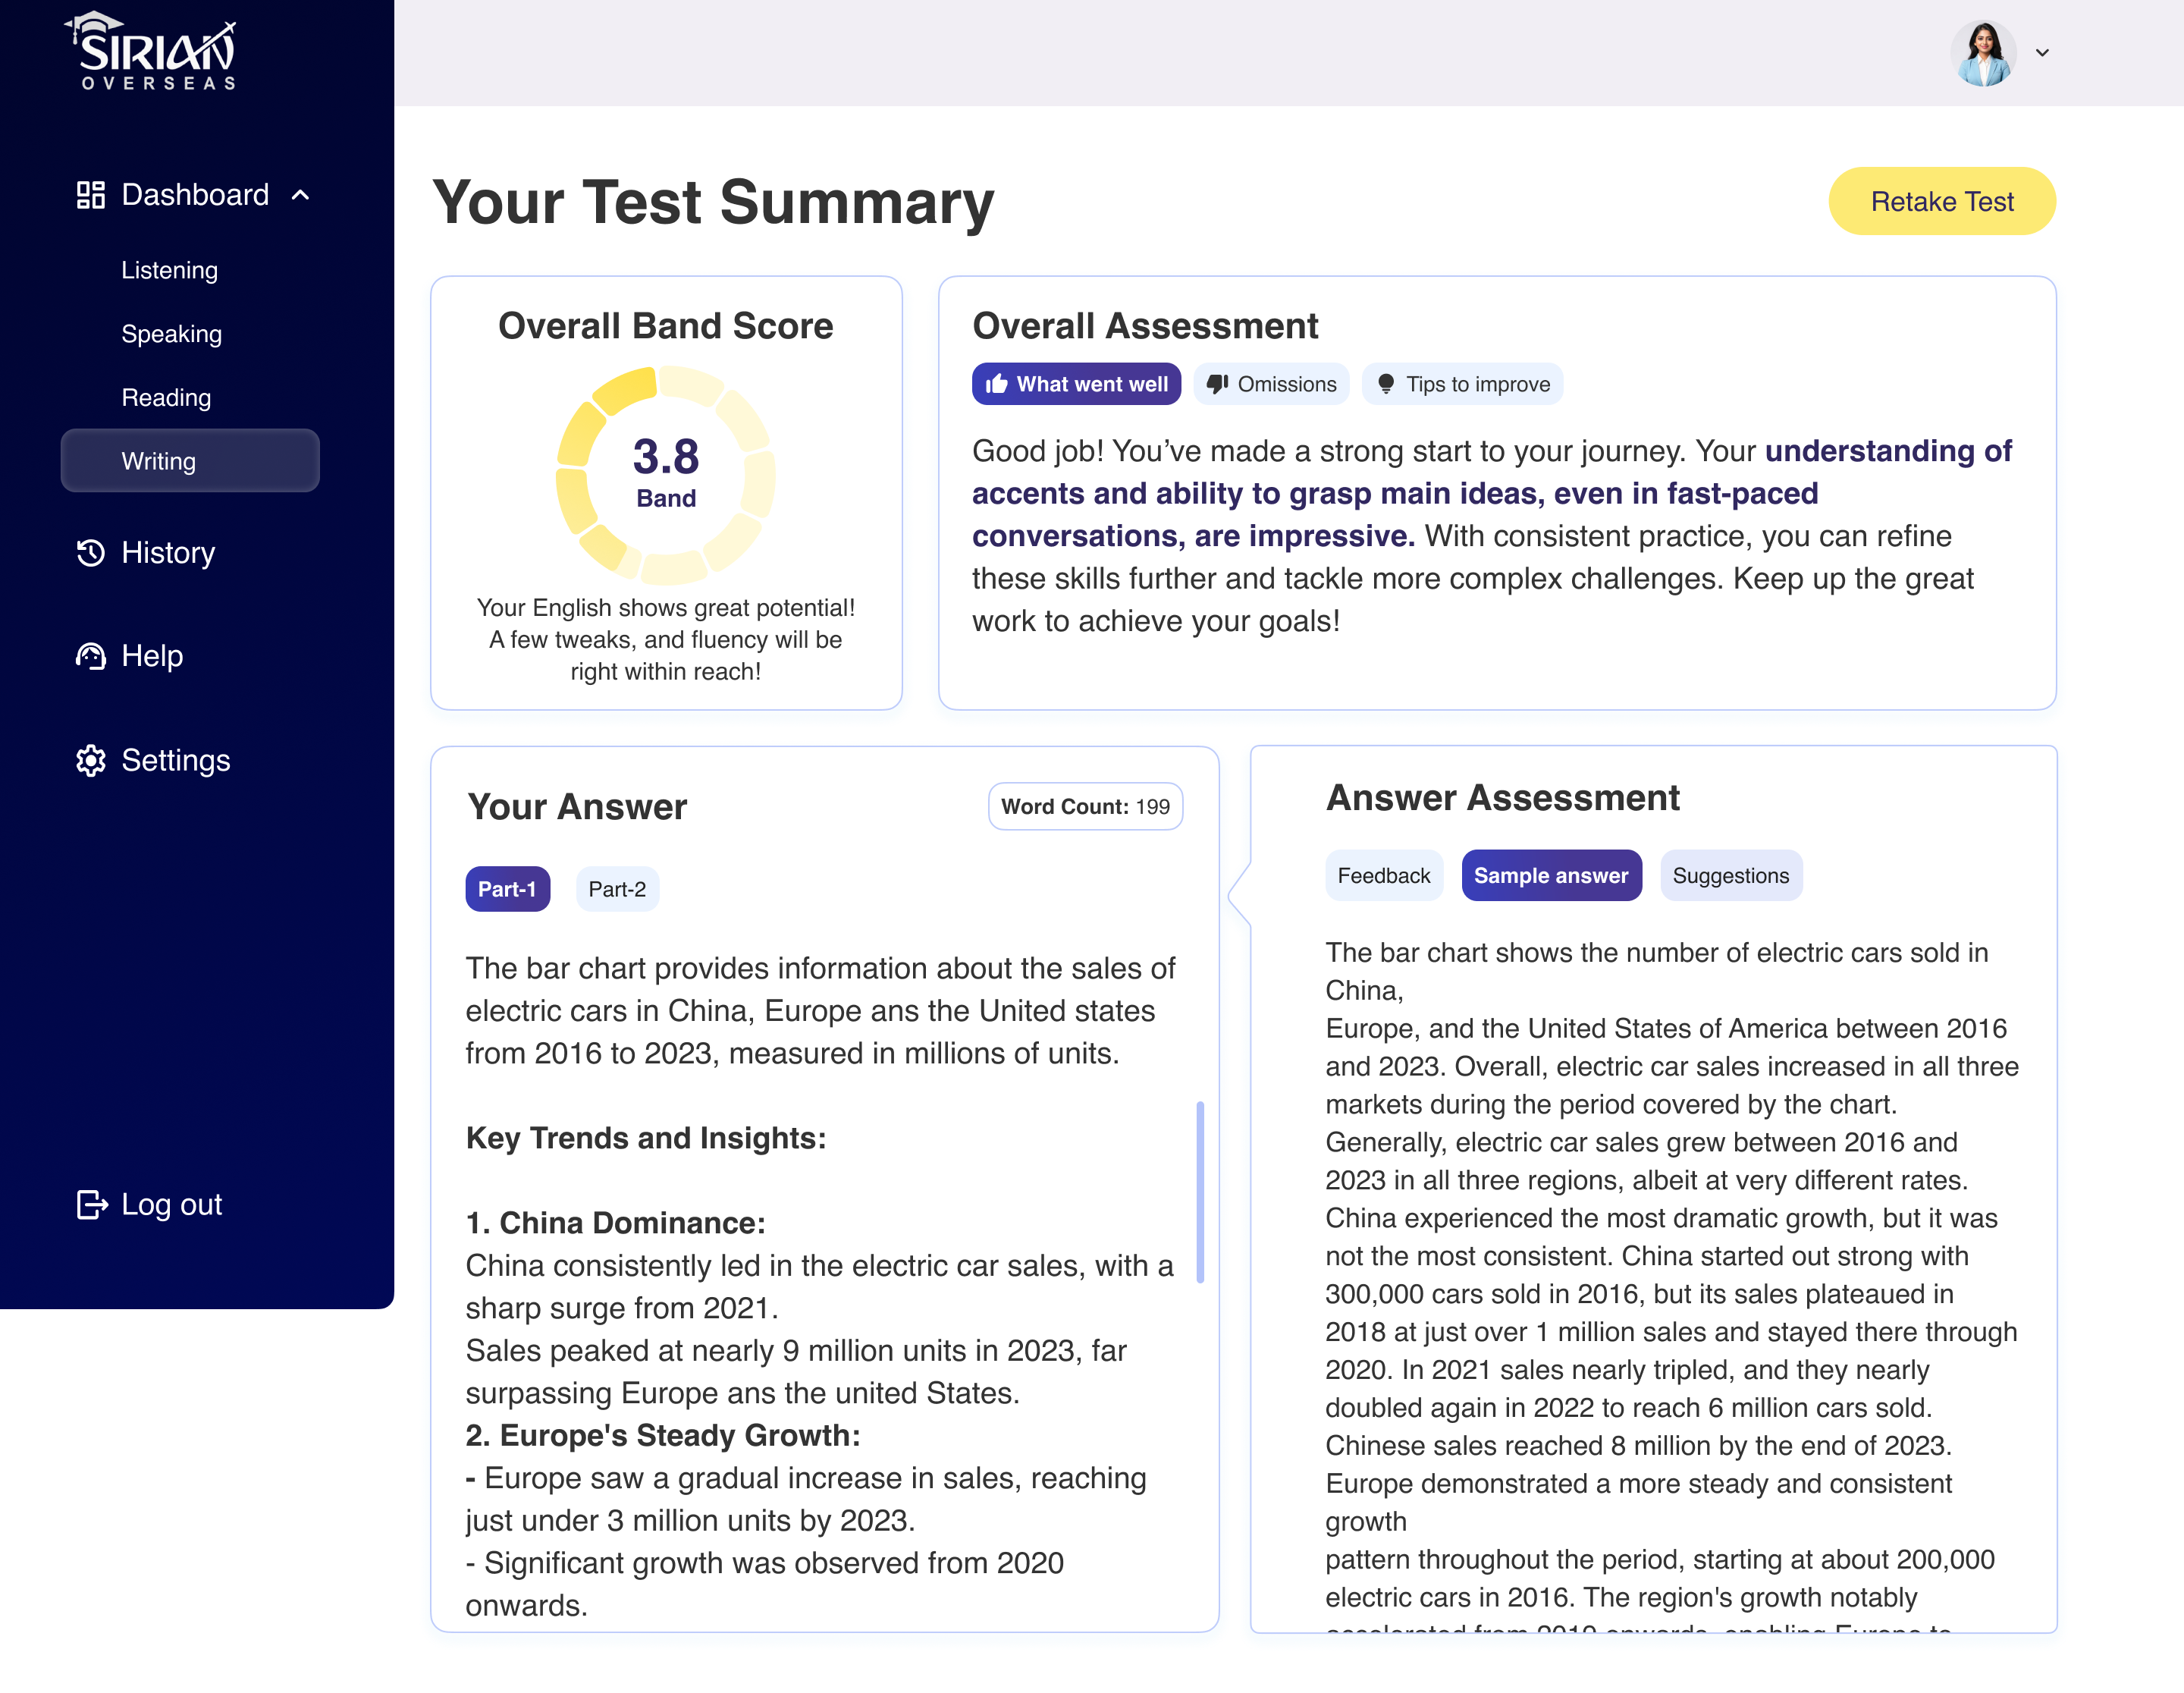
\includegraphics[width=0.8\textwidth]{images/Writing_feedback_page.png}
    \caption{Writing Feedback Generated by AI Engine}
\end{figure}

\vspace{0.3cm}
\subsection{Speaking Module Output}
\begin{itemize}
    \item AI voice-based question delivery works smoothly.
    \item Real-time audio capture and speech-to-text conversion are functional.
    \item Final feedback includes band score and speech accuracy.
\end{itemize}

\begin{figure}[H]
    \centering
    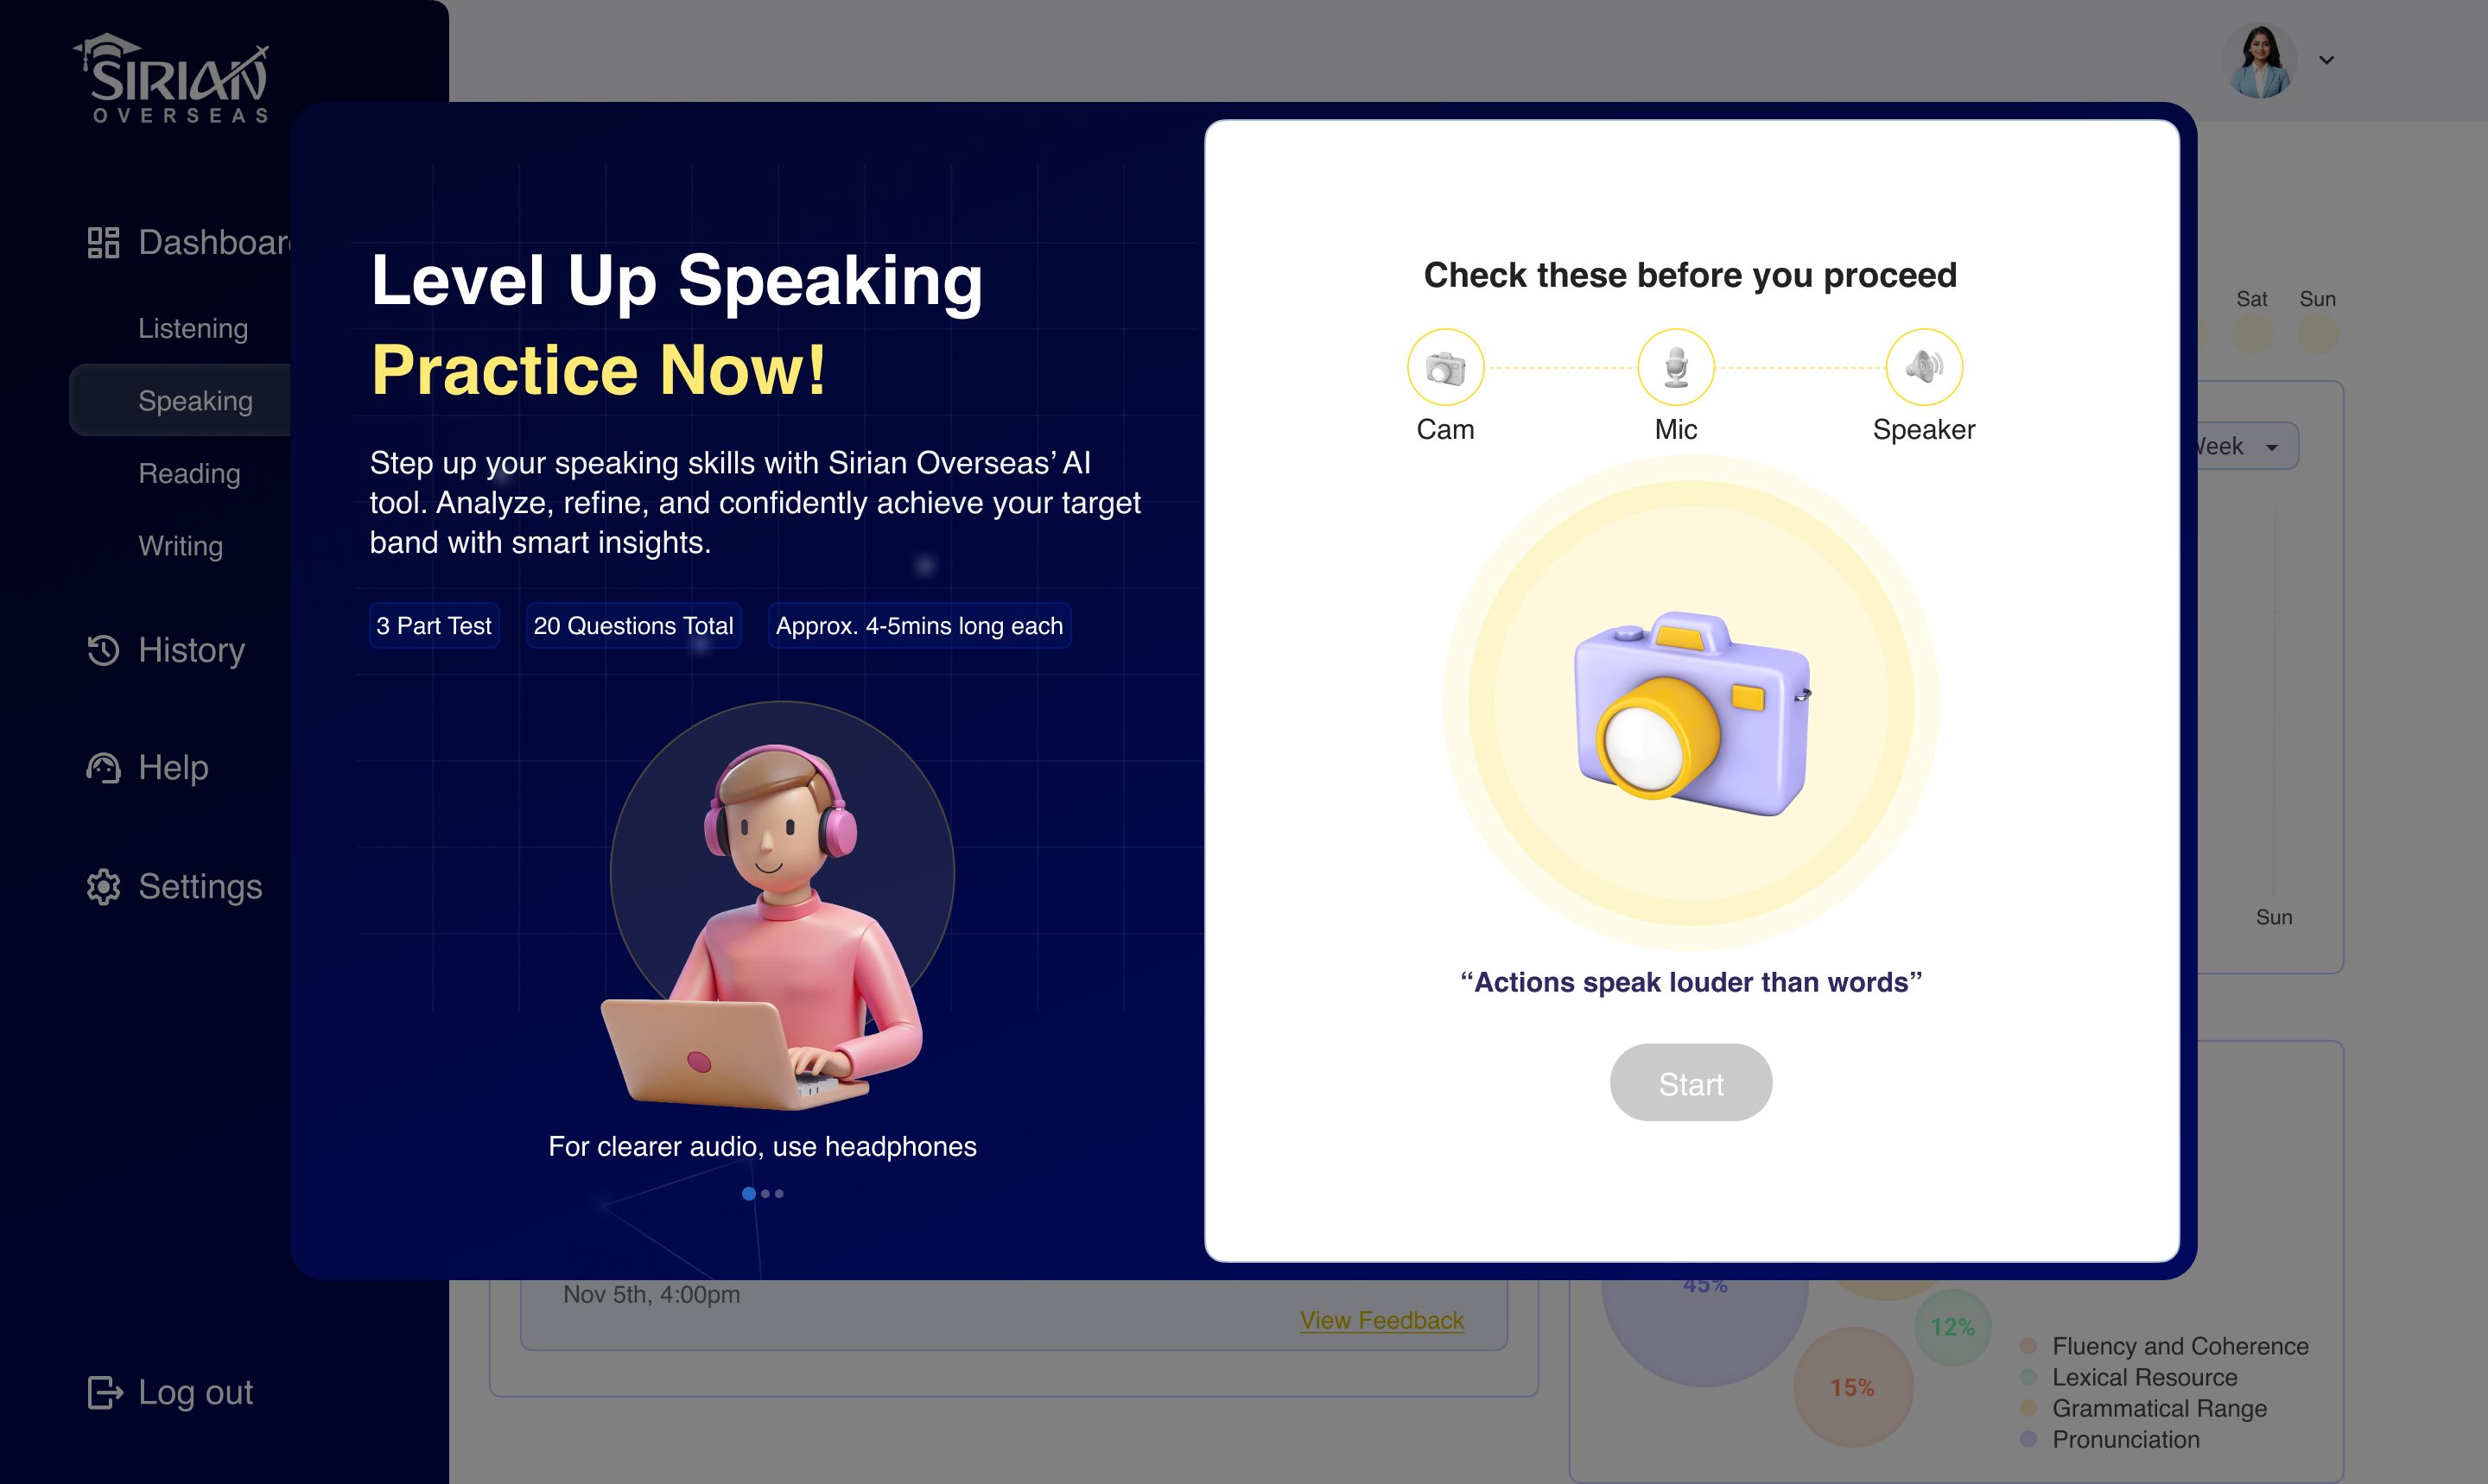
\includegraphics[width=0.8\textwidth]{images/speaking_instructions.png}
    \caption{Speaking Module Instructions and Consent}
\end{figure}

\begin{figure}[H]
    \centering
    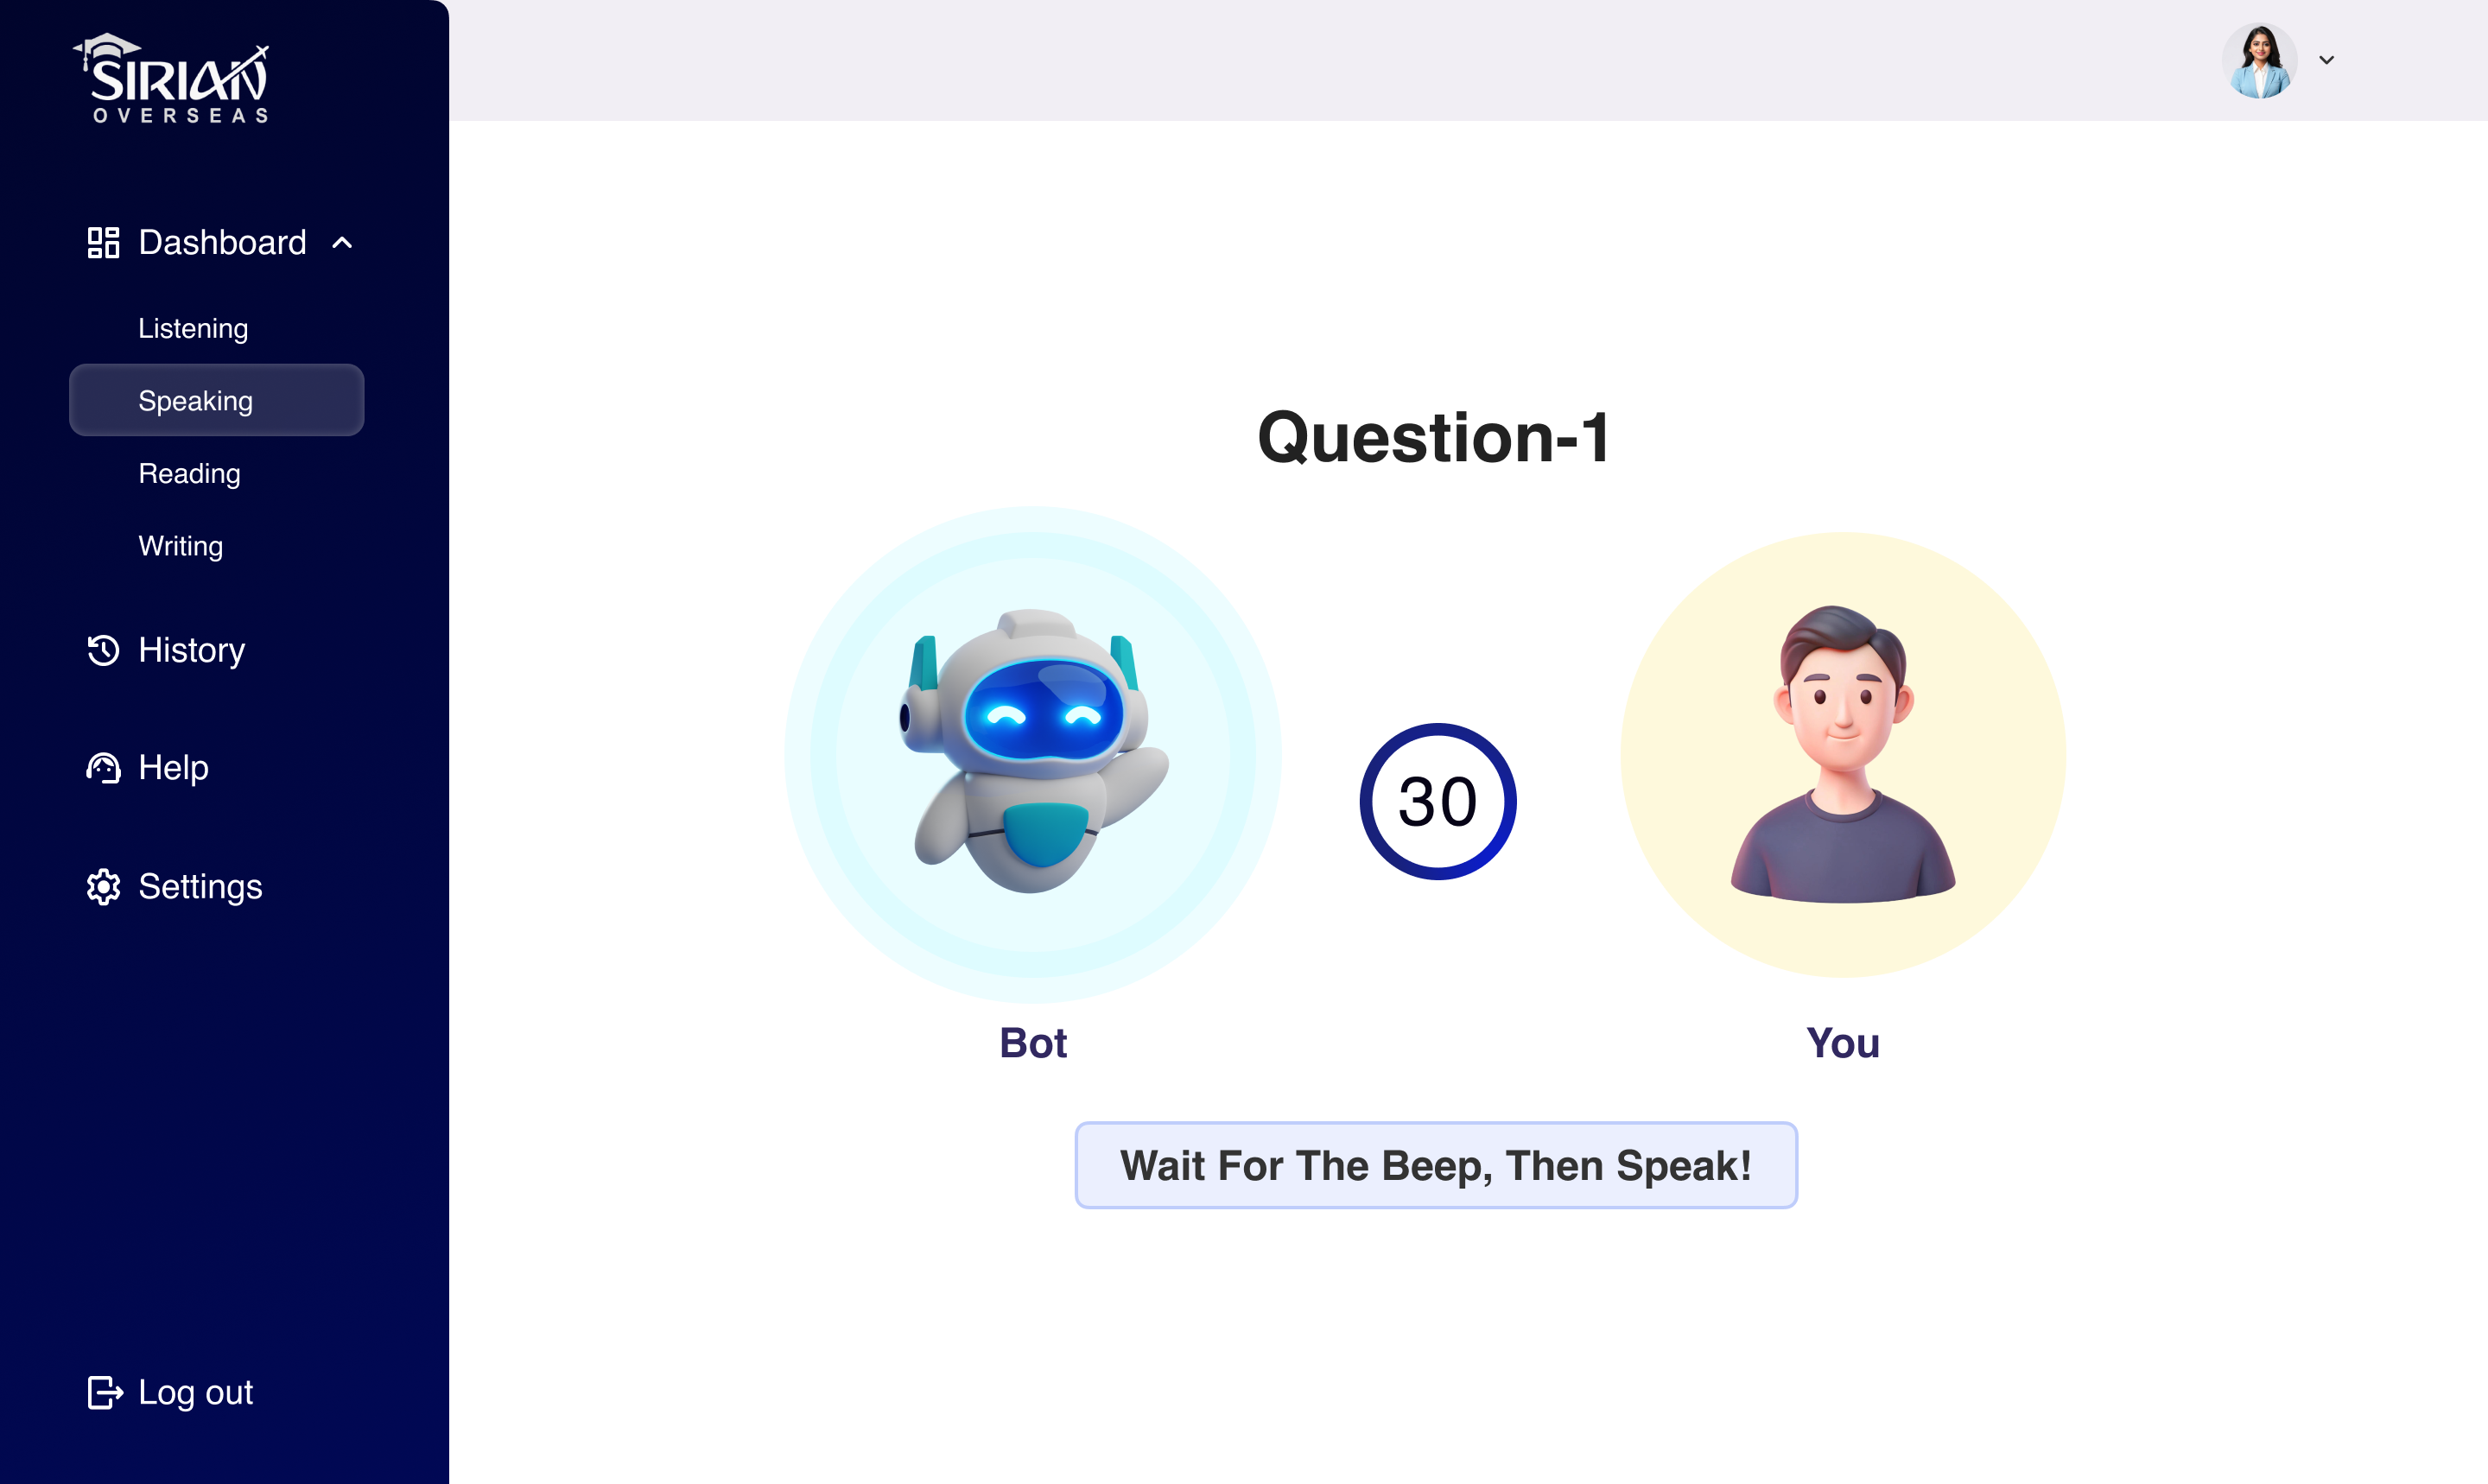
\includegraphics[width=0.8\textwidth]{images/speaking_exam_interface.png}
    \caption{Speaking Test Interface with Recording Timer}
\end{figure}

\begin{figure}[H]
    \centering
    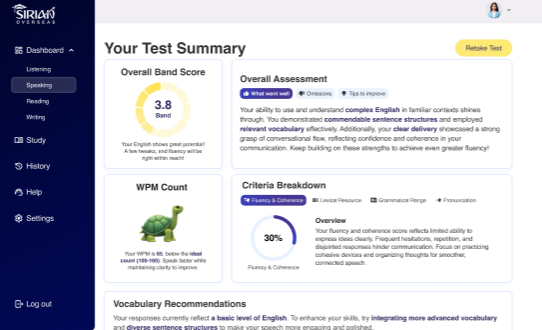
\includegraphics[width=0.8\textwidth]{images/speaking_feedback.png}
    \caption{Speaking Module Band Score and Proficiency Feedback}
\end{figure}

\vspace{0.5cm}
\subsection{Additional Features and Pages}
\textbf{1. Test History Page:} Enables users to view all past test attempts with scores and retake options.

\begin{figure}[H]
    \centering
    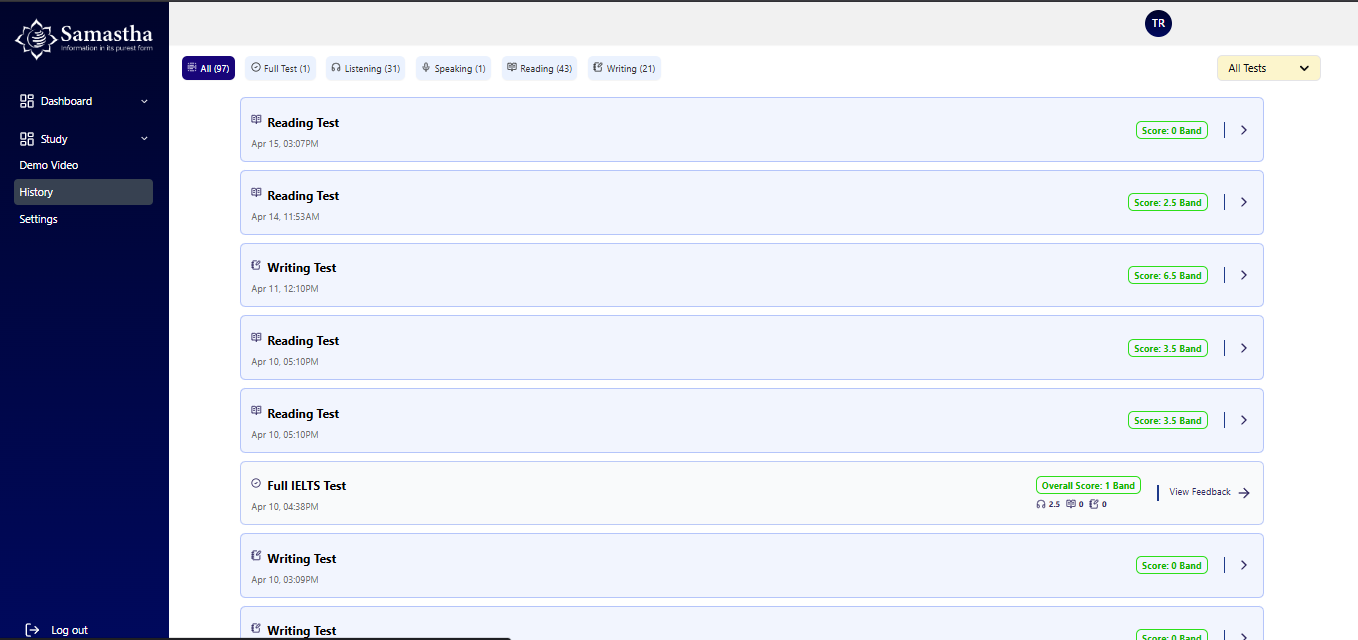
\includegraphics[width=0.8\textwidth]{images/history_page.png}
    \caption{Test History Page with Previous Results}
\end{figure}

\vspace{0.2cm}
\textbf{2. Practice Test Page:} Provides access to module-wise practice without time pressure or evaluation.

\begin{figure}[H]
    \centering
    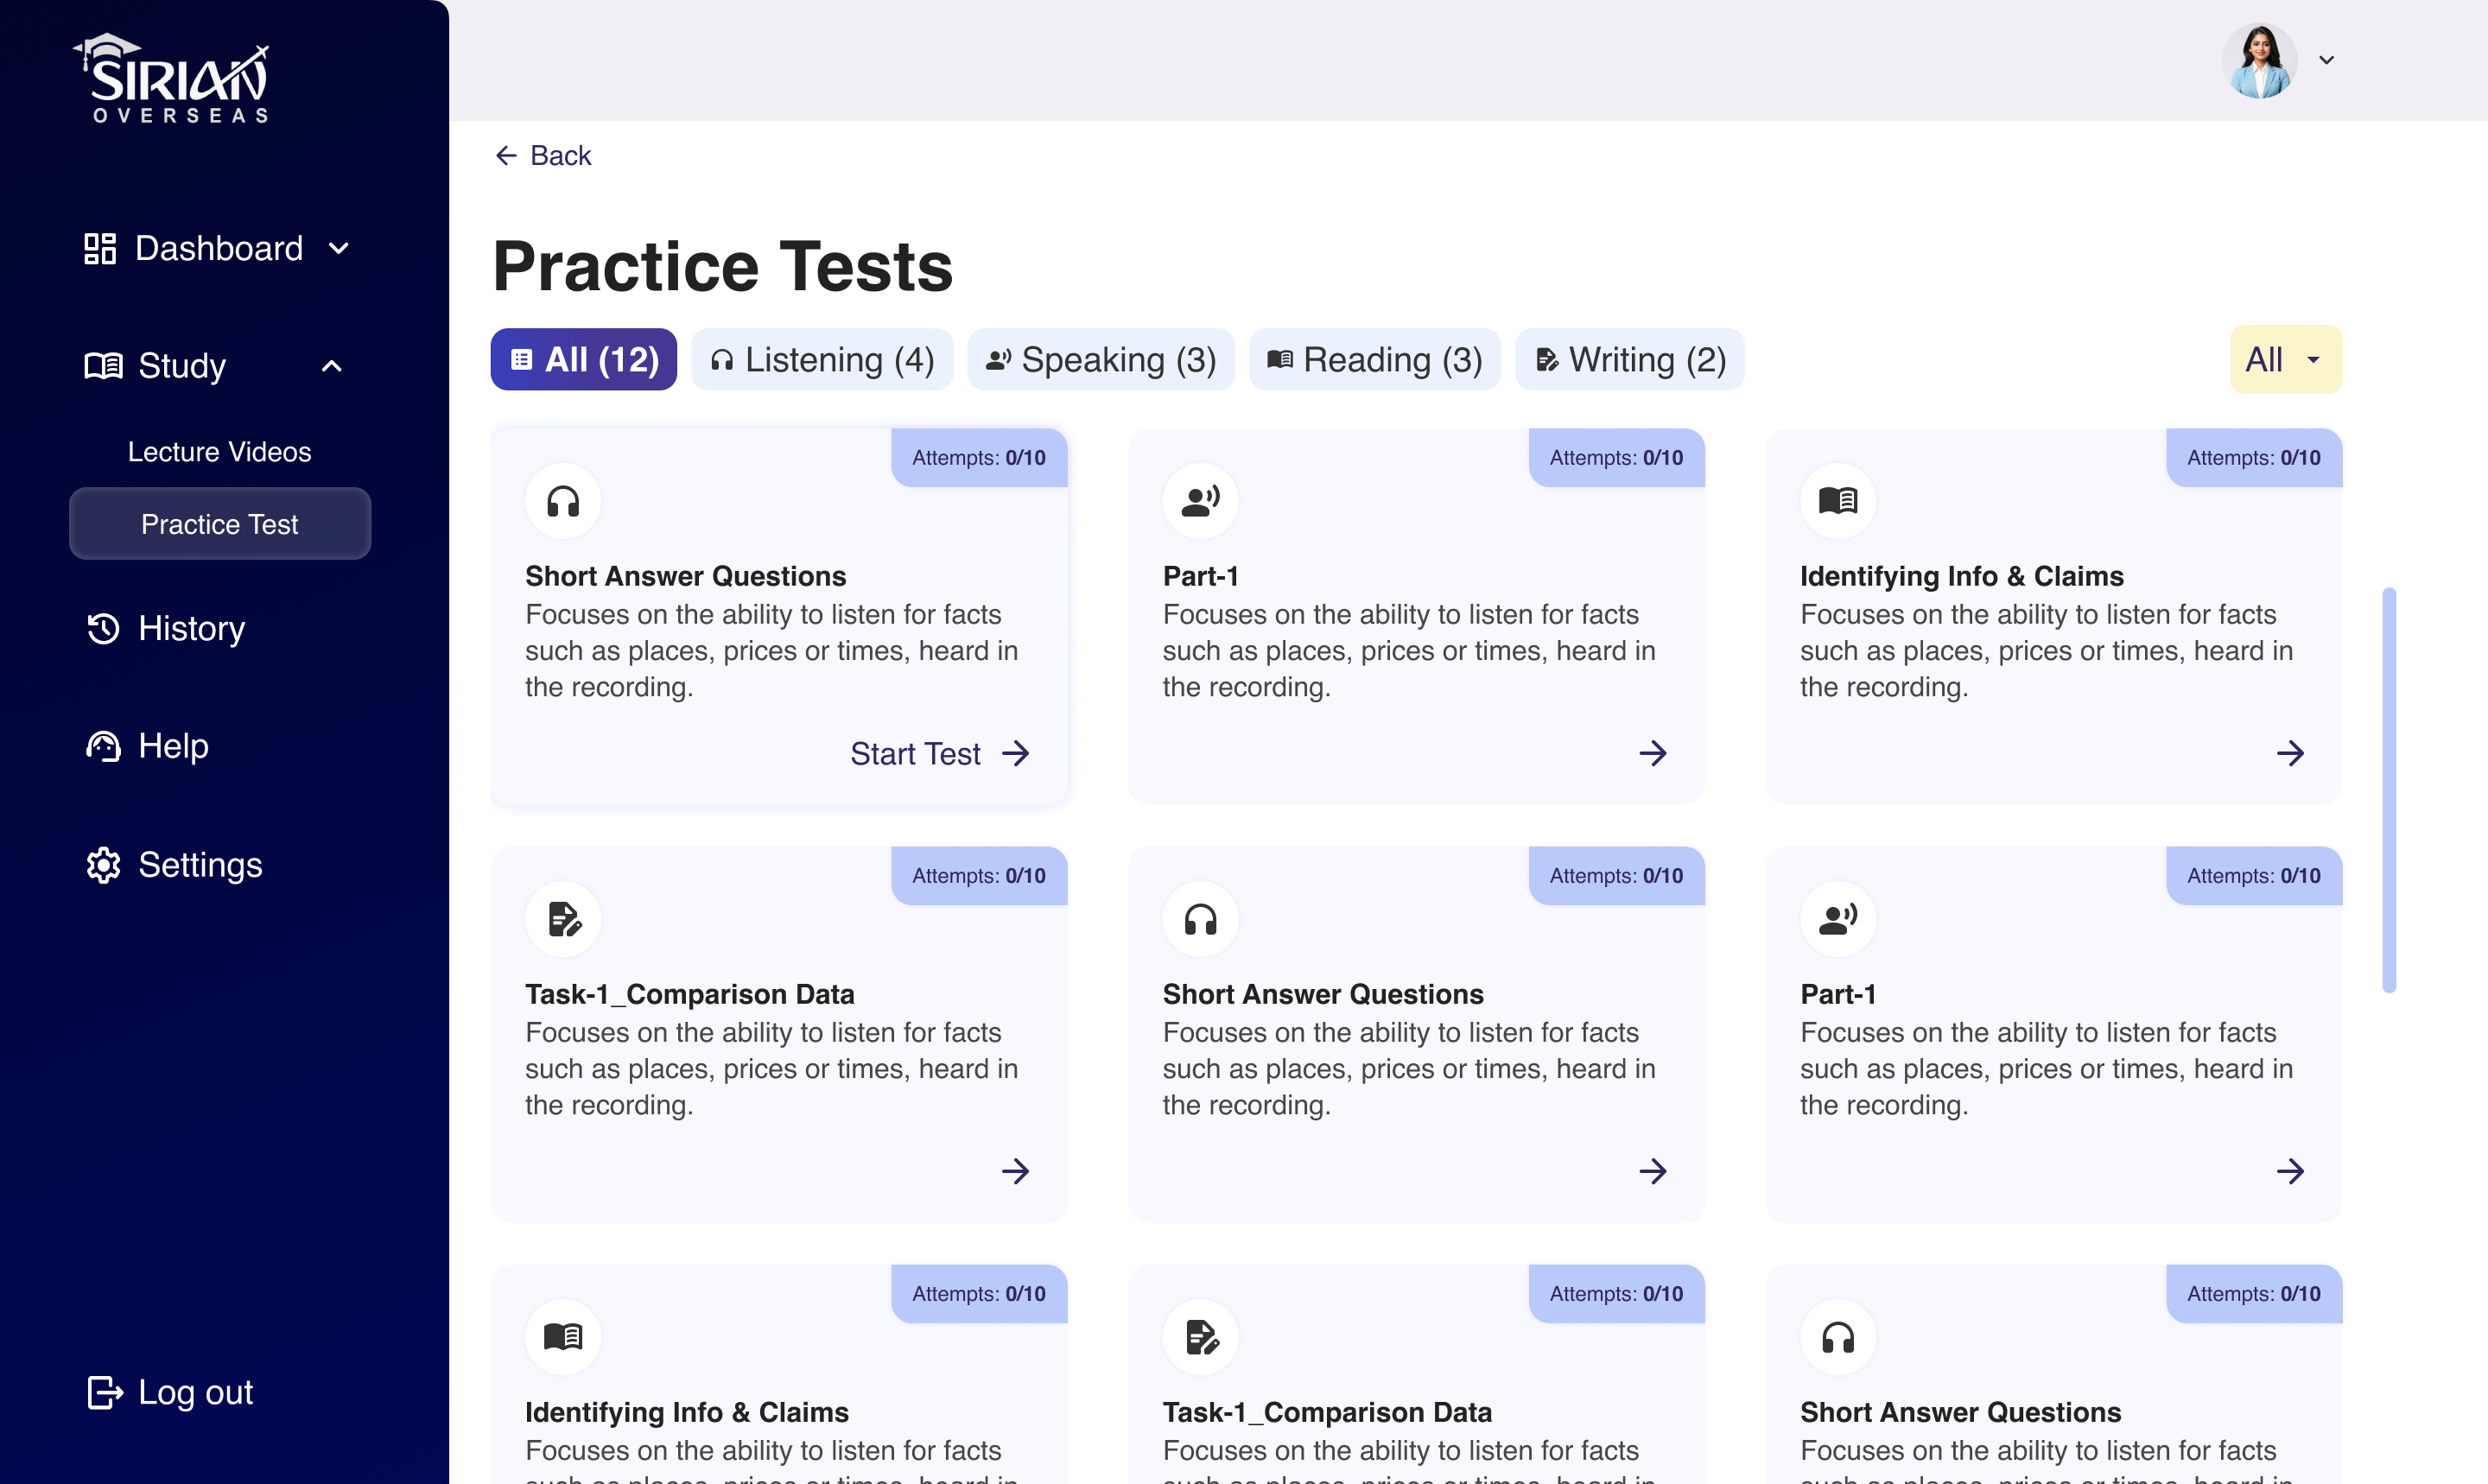
\includegraphics[width=0.8\textwidth]{images/practice_test.png}
    \caption{Practice Test Module Selection}
\end{figure}

\vspace{0.2cm}
\textbf{3. Lecture Videos Page:} Educational video section for test strategies, common mistakes, and grammar review.

\begin{figure}[H]
    \centering
    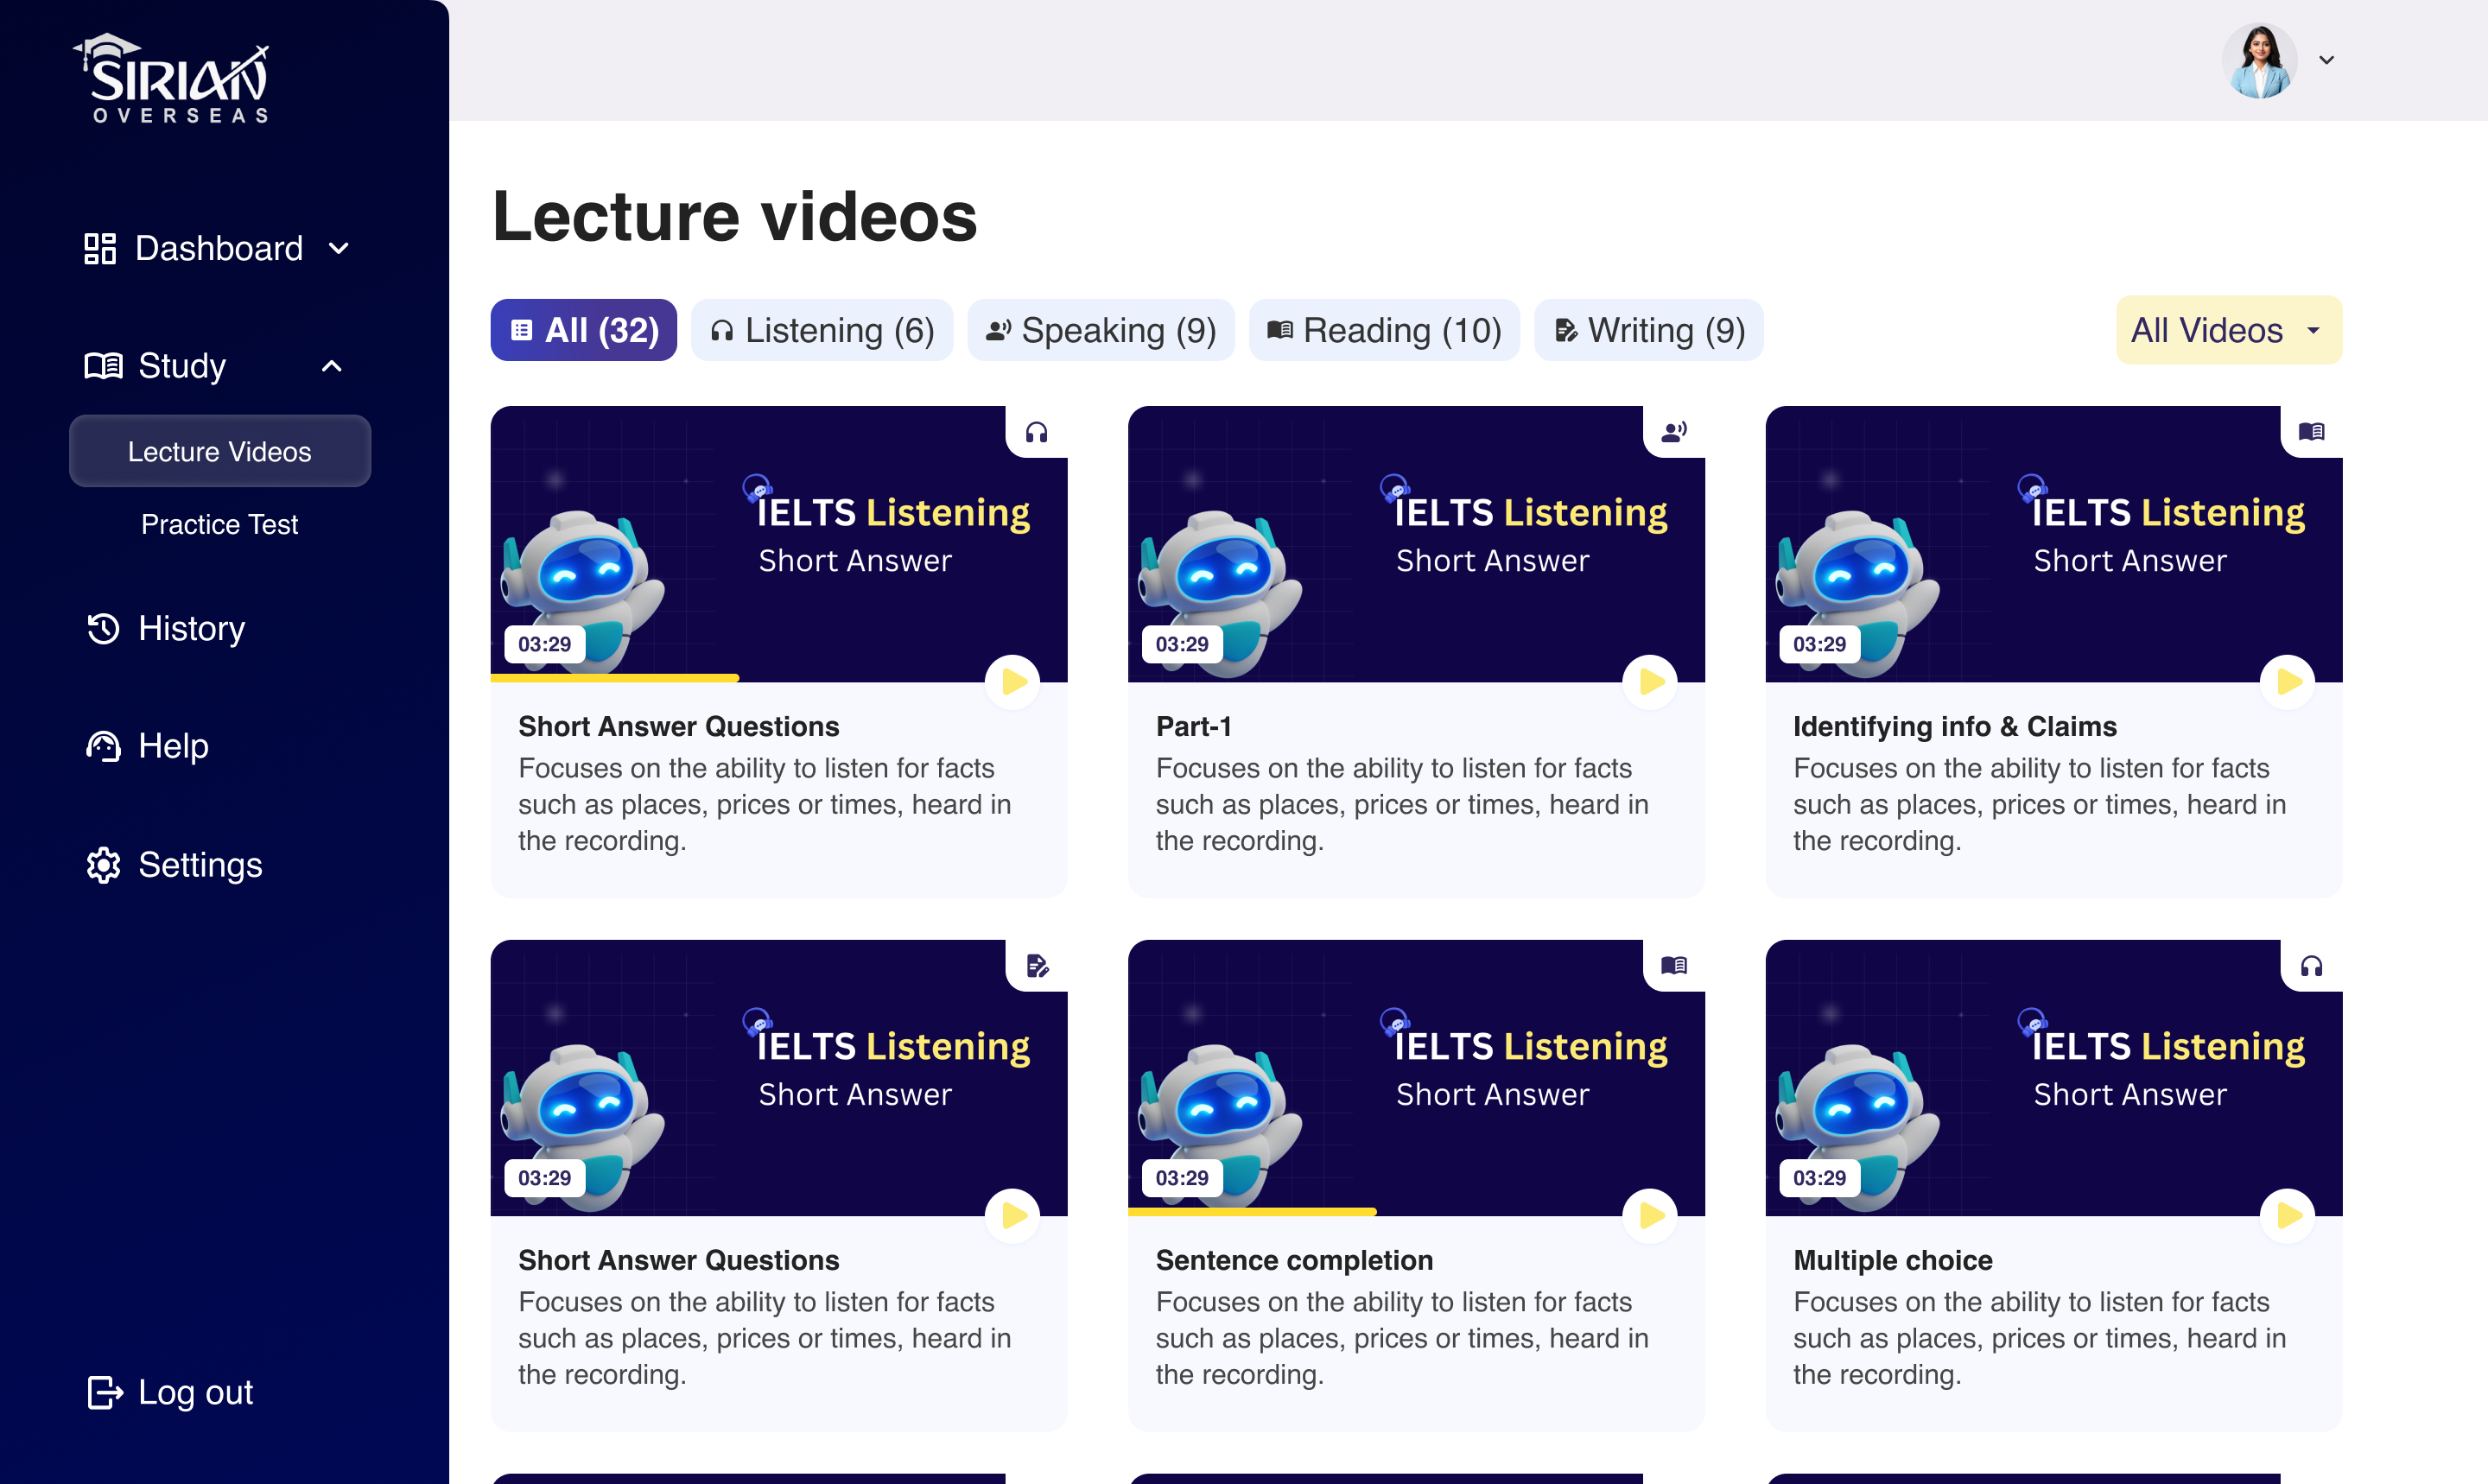
\includegraphics[width=0.8\textwidth]{images/lecture_videos.png}
    \caption{Lecture Videos Page with Subject-wise Content}
\end{figure}

\vspace{0.5cm}
\subsection{Performance Observations}
The system was tested under standard conditions and yielded the following:
\begin{itemize}
    \item Minimal latency observed in AI-based feedback modules.
    \item Consistent UI rendering and media playback across browsers.
    \item All answers stored and retrieved accurately for history and analytics.
\end{itemize}

\vspace{0.5cm}
The module-wise outputs and system behavior confirm full alignment with the functional goals outlined in the FRD, affirming the readiness of the platform for real-world IELTS test preparation.



%------------------------------------- CONCLUSION -------------------------------------%
\newpage
\section{Conclusion}
% \addcontentsline{toc}{section}{Conclusion}

\vspace{0.5cm}

The development of \textbf{SAMASTHA - IELTS MOCK} has proven to be a significant milestone in providing a modern, AI-enhanced platform that aims to revolutionize IELTS exam preparation. This project was driven by the need for a more personalized, accessible, and interactive way for test-takers to prepare for the IELTS exam. With the increasing reliance on technology in educational tools, \textbf{SAMASTHA - IELTS MOCK} stands as a forward-thinking solution that offers a comprehensive approach to simulating real-world testing environments and delivering timely, personalized feedback, thus helping learners optimize their preparation for the exam.

\vspace{0.3cm}

At the core of this platform's design was the intention to create a highly functional, easy-to-use, and engaging learning experience. The development process involved deep consideration of various facets essential to the IELTS exam preparation journey. The platform not only mirrors authentic IELTS testing conditions but also integrates innovative technologies to provide continuous feedback and track user progress. This ensures a holistic approach to learning that empowers users to take charge of their study schedules, identifying and addressing weak areas as they prepare for one of the most significant academic and professional exams worldwide.

\vspace{0.3cm}

A significant portion of the platform’s success lies in the successful implementation of the following key aspects:
\begin{itemize}
    \item \textbf{Simulation of Authentic IELTS Exam Conditions:} The platform is designed to replicate the official IELTS exam’s four modules — Listening, Reading, Writing, and Speaking — to provide an experience that is as close as possible to the real test. This not only reduces the anxiety typically experienced by exam-takers but also helps familiarize them with the format and structure of the test, leading to better preparedness.
    \item \textbf{Responsive and Seamless User Interface:} A strong focus was placed on creating an intuitive, user-friendly interface that adapts well across various devices, ensuring that users can access the platform comfortably from their desktops, tablets, or smartphones. This cross-device compatibility enhances the flexibility of the learning process, allowing users to continue their preparations anytime and anywhere.
    \item \textbf{AI-Powered Dynamic Evaluation and Feedback:} One of the most innovative aspects of the platform is its integration with AI technologies, such as OpenAI for generating dynamic feedback and Google Speech API for assessing speaking responses. This combination allows for real-time evaluation of user input, providing instant, personalized feedback on areas for improvement. By simulating actual exam conditions, the AI not only gives constructive feedback but also helps users enhance their time management skills by replicating the time constraints of the real exam.
    \item \textbf{Detailed Analytics and Progress Tracking:} The analytics dashboard is another cornerstone of the platform’s design. It serves as a comprehensive tool for tracking the user’s performance over time. This module consolidates scores, progress data, and feedback to create a visual representation of the user’s growth, allowing them to identify trends, track improvements, and adjust their study plan accordingly. By understanding their strengths and weaknesses through detailed data, users can make informed decisions about their study priorities.
\end{itemize}

\vspace{0.3cm}

The Listening, Reading, Writing, and Speaking modules were developed with a high degree of accuracy, reflecting the official IELTS exam structure. In particular, the use of real-time feedback through AI-powered mechanisms, such as the integration of OpenAI and Google Speech APIs, enhanced the platform’s ability to provide immediate corrective advice, a feature that is typically difficult to replicate in traditional study methods. By offering such timely feedback, users are able to assess their performance as they go, without the need to wait for manual scoring or evaluation.

\vspace{0.3cm}

The dashboard is another feature that enhances the learning process. It serves not only as a repository for scores and past attempts but also as an insightful analytics tool that highlights areas for improvement, offering users the ability to make data-driven decisions about their learning journey. This gives users control over their preparation, helping them strategize and focus their efforts on improving weaker areas rather than repeating areas where they already perform well.

\vspace{0.3cm}

From both a technical and functional perspective, the platform underwent rigorous testing and validation against the Functional Requirements Document (FRD) to ensure all features performed as intended. The platform was evaluated in terms of accuracy, usability, system performance, and overall effectiveness. Its ability to meet the defined functional and academic goals confirms its viability as a reliable tool for learners worldwide.

\vspace{0.3cm}

While this project achieves its immediate academic and functional goals, it also demonstrates immense potential for future growth and expansion. The platform could be further developed into a deployable product for wider use, with potential extensions such as mobile applications, adaptive testing features, and personalized teacher dashboards for managing student progress. These future enhancements could significantly broaden the platform’s scope, enabling it to cater to a wider audience and become a leading AI-powered language learning tool.

\vspace{0.3cm}

In conclusion, \textbf{SAMASTHA - IELTS MOCK} exemplifies the powerful convergence of artificial intelligence, thoughtful user experience (UX) design, and structured pedagogical strategies. It showcases how modern technology can enhance traditional learning processes, making exam preparation more efficient, personalized, and less stressful for users. The integration of cutting-edge AI, paired with a seamless and intuitive interface, offers a unique and comprehensive solution that reshapes the way learners prepare for high-stakes exams like the IELTS. This project stands as a testament to the future of educational tools, combining innovation, usability, and impact to meet the evolving needs of learners in a rapidly digitalizing world.



%------------------------------------ REFERENCES -------------------------------------%
\newpage
\section{References}

\vspace{0.5cm}

\begin{enumerate}
    \renewcommand{\labelenumi}{[\theenumi]}
    
    \item Figma Design for UI/UX Planning — \\
    \textit{TEST PREP AI TOOLS}: \\
    \url{https://www.figma.com/design/9f2Ea52IGTKrhAiZyGWPkn/TEST-PREP-AI-TOOLS?node-id=2315-214}

    \item Google Cloud Speech-to-Text API Documentation — \\
    \url{https://cloud.google.com/speech-to-text/docs}

    \item OpenAI GPT API Documentation — \\
    \url{https://platform.openai.com/docs}

    \item MySQL Official Documentation — \\
    \url{https://dev.mysql.com/doc/}

    \item React.js Official Docs — \\
    \url{https://reactjs.org/docs/getting-started.html}

    \item Tailwind CSS Documentation — \\
    \url{https://tailwindcss.com/docs}

    \item Python FastAPI Documentation — \\
    \url{https://fastapi.tiangolo.com/}
    \\
    
    Guided throughout the documentation, architecture design, LaTeX formatting, and technical articulation. ��
\end{enumerate}



% %-----------------------------GITHUB-----------------------------------------------------%

% \newpage
% \section*{GitHub Repository}
% \vspace{1cm}

% We are excited to share the source code, documentation, and the presentation slides for the \textbf{SAMASTHA - IELTS MOCK} project! You can access everything in our GitHub repository using the link below:

% \begin{center}
%     \textbf{\href{https://github.com/your-github-link}{https://github.com/your-github-link}} 
% \end{center}

% \vspace{0.5cm}

% This repository contains:
% \begin{itemize}
%     \item The complete source code for the platform.
%     \item A detailed documentation of the development process.
%     \item The PowerPoint presentation that summarizes the project.
% \end{itemize}

% \vspace{0.5cm}

% Feel free to explore, clone, and contribute! We encourage you to dive into the project, make improvements, and share your ideas. The journey doesn’t end here — let's keep pushing the boundaries of what technology can do in the world of education.

% \vspace{0.5cm}

% Let’s continue to innovate, inspire, and make learning smarter for everyone! The future of AI-powered education starts with projects like this — and who knows? You might just be the one to take it to the next level. ��

% \vspace{0.5cm}
% \hspace{4cm} \textit{Together, we can make a difference in how the world learns!}



%---------------------------------------------------------------------------%

\end{document}
